% UCL Thesis LaTeX Template
%  (c) Ian Kirker, 2014
% 
% This is a template/skeleton for PhD/MPhil/MRes theses.
%
% It uses a rather split-up file structure because this tends to
%  work well for large, complex documents.
% We suggest using one file per chapter, but you may wish to use more
%  or fewer separate files than that.
% We've also separated out various bits of configuration into their
%  own files, to keep everything neat.
% Note that the \input command just streams in whatever file you give
%  it, while the \include command adds a page break, and does some
%  extra organisation to make compilation faster. Note that you can't
%  use \include inside an \include-d file.
% We suggest using \input for settings and configuration files that
%  you always want to use, and \include for each section of content.
% If you do that, it also means you can use the \includeonly statement
%  to only compile up the section you're currently interested in.
% You might also want to put figures into their own files to be \input.

% For more information on \input and \include, see:
%  http://tex.stackexchange.com/questions/246/when-should-i-use-input-vs-include


% Formatting and binding rules for theses are here: 
%  https://www.ucl.ac.uk/students/exams-and-assessments/research-assessments/format-bind-and-submit-your-thesis-general-guidance

% This package goes first and foremost, because it checks all 
%  your syntax for mistakes and some old-fashioned LaTeX commands.
% Note that normally you should load your documentclass before 
%  packages, because some packages change behaviour based on
%  your document settings.
% Also, for those confused by the RequirePackage here vs usepackage
%  elsewhere, usepackage cannot be used before the documentclass
%  command, while RequirePackage can. That's the only functional
%  difference as far as I'm aware.
\RequirePackage[l2tabu, orthodox]{nag}


% ------ Main document class specification ------
% The draft option here prevents images being inserted,
%  and adds chunky black bars to boxes that are exceeding 
%  the page width (to show that they are).
% The oneside option can optionally be replaced by twoside if
%  you intend to print double-sided. Note that this is
%  *specifically permitted* by the UCL thesis formatting
%  guidelines.
%
% Valid options in terms of type are:
%  phd
%  mres
%  mphil
%\documentclass[12pt,phd,draft,a4paper,oneside]{ucl_thesis}
\documentclass[12pt,phd,a4paper,oneside]{ucl_thesis}


% Package configuration:
%  LaTeX uses "packages" to add extra commands and features.
%  There are quite a few useful ones, so we've put them in a 
%   separate file.
% -------- Packages --------

% This package just gives you a quick way to dump in some sample text.
% You can remove it -- it's just here for the examples.
\usepackage{blindtext}

% This package means empty pages (pages with no text) won't get stuff
%  like chapter names at the top of the page. It's mostly cosmetic.
\usepackage{emptypage}

% The graphicx package adds the \includegraphics command,
%  which is your basic command for adding a picture.
\usepackage{graphicx}

% The float package improves LaTeX's handling of floats,
%  and also adds the option to *force* LaTeX to put the float
%  HERE, with the [H] option to the float environment.
\usepackage{float}

% The amsmath package enhances the various ways of including
%  maths, including adding the align environment for aligned
%  equations.
\usepackage{amsmath}

% Use these two packages together -- they define symbols
%  for e.g. units that you can use in both text and math mode.
\usepackage{gensymb}
\usepackage{textcomp}
% You may also want the units package for making little
%  fractions for unit specifications.
%\usepackage{units}


% The setspace package lets you use 1.5-sized or double line spacing.
\usepackage{setspace}
\setstretch{1.5}

% That just does body text -- if you want to expand *everything*,
%  including footnotes and tables, use this instead:
%\renewcommand{\baselinestretch}{1.5}


% PGFPlots is either a really clunky or really good way to add graphs
%  into your document, depending on your point of view.
% There's waaaaay too much information on using this to cover here,
%  so, you might want to start here:
%   http://pgfplots.sourceforge.net/
%  or here:
%   http://pgfplots.sourceforge.net/pgfplots.pdf
%\usepackage{pgfplots}
%\pgfplotsset{compat=1.3} % <- this fixed axis labels in the version I was using

% PGFPlotsTable can help you make tables a little more easily than
%  usual in LaTeX.
% If you're going to have to paste data in a lot, I'd suggest using it.
%  You might want to start with the manual, here:
%  http://pgfplots.sourceforge.net/pgfplotstable.pdf
%\usepackage{pgfplotstable}

% These settings are also recommended for using with pgfplotstable.
%\pgfplotstableset{
%	% these columns/<colname>/.style={<options>} things define a style
%	% which applies to <colname> only.
%	empty cells with={--}, % replace empty cells with '--'
%	every head row/.style={before row=\toprule,after row=\midrule},
%	every last row/.style={after row=\bottomrule}
%}


% The mhchem package provides chemistry formula typesetting commands
%  e.g. \ce{H2O}
%\usepackage[version=3]{mhchem}

% And the chemfig package gives a weird command for adding Lewis 
%  diagrams, for e.g. organic molecules
%\usepackage{chemfig}

% The linenumbers command from the lineno package adds line numbers
%  alongside your text that can be useful for discussing edits 
%  in drafts.
% Remove or comment out the command for proper versions.
%\usepackage[modulo]{lineno}
% \linenumbers 


% Alternatively, you can use the ifdraft package to let you add
%  commands that will only be used in draft versions
%\usepackage{ifdraft}

% For example, the following adds a watermark if the draft mode is on.
%\ifdraft{
%  \usepackage{draftwatermark}
%  \SetWatermarkText{\shortstack{\textsc{Draft Mode}\\ \strut \\ \strut \\ \strut}}
%  \SetWatermarkScale{0.5}
%  \SetWatermarkAngle{90}
%}


% The multirow package adds the option to make cells span 
%  rows in tables.
\usepackage{multirow}

\usepackage{bookmark}
% Subfig allows you to create figures within figures, to, for example,
%  make a single figure with 4 individually labeled and referenceable
%  sub-figures.
% It's quite fiddly to use, so check the documentation.
%\usepackage{subfig}

% The natbib package allows book-type citations commonly used in
%  longer works, and less commonly in science articles (IME).
% e.g. (Saucer et al., 1993) rather than [1]
% More details are here: http://merkel.zoneo.net/Latex/natbib.php
%\usepackage{natbib}

% The bibentry package (along with the \nobibliography* command)
%  allows putting full reference lines inline.
%  See: 
%   http://tex.stackexchange.com/questions/2905/how-can-i-list-references-from-bibtex-file-in-line-with-commentary
\usepackage{bibentry} 

% The isorot package allows you to put things sideways 
%  (or indeed, at any angle) on a page.
% This can be useful for wide graphs or other figures.
%\usepackage{isorot}

% The caption package adds more options for caption formatting.
% This set-up makes hanging labels, makes the caption text smaller
%  than the body text, and makes the label bold.
% Highly recommended.
\usepackage[format=hang,font=small,labelfont=bf]{caption}

% If you're getting into defining your own commands, you might want
%  to check out the etoolbox package -- it defines a few commands
%  that can make it easier to make commands robust.
\usepackage{etoolbox}

% The microtype package adds `micro-typographic extensions' which
% generally makes text more readable and hyphenation less likely.
\usepackage{microtype}
\usepackage{enumitem}
\usepackage{makecell}

% Sets up links within your document, for e.g. contents page entries
%  and references, and also PDF metadata.
% You should edit this!
%%
%% This file uses the hyperref package to make your thesis have metadata embedded in the PDF, 
%%  and also adds links to be able to click on references and contents page entries to go to 
%%  the pages.
%%

% Some hacks are necessary to make bibentry and hyperref play nicely.
% See: http://tex.stackexchange.com/questions/65348/clash-between-bibentry-and-hyperref-with-bibstyle-elsart-harv
\usepackage{bibentry}
\makeatletter\let\saved@bibitem\@bibitem\makeatother
% \usepackage[pdftex,hidelinks]{hyperref}
\usepackage{hyperref}
\makeatletter\let\@bibitem\saved@bibitem\makeatother
\makeatletter
\AtBeginDocument{
    \hypersetup{
        pdfsubject={Thesis Subject},
        pdfkeywords={Thesis Keywords},
        pdfauthor={Author},
        pdftitle={Title},
    }
}
\makeatother
    


% And then some settings in separate files.
\input{FloatSettings} % For things like figures and tables
\bibliographystyle{unsrt}
   % For bibliographies

% These control how many number sections your subsections will take
%    e.g. Section 2.3.1.5.6.3
%  and how many of those will get put into the contents pages.
\setcounter{secnumdepth}{3}
\setcounter{tocdepth}{3}


\begin{document}

\nobibliography*
% ^-- This is a dumb trick that works with the bibentry package to let
%  you put bibliography entries whereever you like.
% I used this to put references to papers a chapter's work was 
%  published in at the end of that chapter.
% For more information, see: http://stefaanlippens.net/bibentry

% If you haven't finished making your full BibTex file yet, you
%  might find this useful -- it'll just replace all your
%  citations with little superscript notes.
% Uncomment to use.
%\renewcommand{\cite}[1]{\emph{\textsuperscript{[#1]}}}

% At last, content! Remember filenames are case-sensitive and 
%  *must not* include spaces.
% I may change the way this is done in a future version, 
%  but given that some people needed it, if you need a different degree title 
%  (e.g. Master of Science, Master in Science, Master of Arts, etc)
%  uncomment the following 3 lines and set as appropriate (this *has* to be before \maketitle)
% \makeatletter
% \renewcommand {\@degree@string} {Master of Things}
% \makeatother

\title{Multimodal Data Fusion for Motor Neuron Disease Prognosis Prediction}
\author{Florence J Townend}
\department{Centre for Medical Image Computing and Institute of Health Informatics}

\maketitle
\makedeclaration

\begin{abstract} % 300 word limit

    Motor neuron disease (MND) is a rare neurodegenerative disease with no cure and clinically heterogeneous progression and presentation.
    Accurate prognosis prediction is crucial for patient care and clinical trial planning, predominantly relying on clinical data. 
    Incorporating neuroimaging data as well could enhance prognostic accuracy.
    This thesis explores the use of multimodal data for prognosis prediction in MND, aiming to improve survival prediction accuracy by combining clinical and neuroimaging data through machine learning techniques, known as multimodal data fusion.

    We investigated how multimodal data affects a simple survival analysis technique, the Cox proportional hazards model, revealing significant predictors of MND survival across both clinical and neuroimaging-derived variables.
    We then explored how more complex machine learning models can be used to predict survival in MND, aiming to capture the complex relationships between the different data modalities through deep learning.
    Since the architectures of multimodal deep learning models vary significantly, we developed a Python library, Fusilli, a tool for comparing different multimodal architectures.
    We used Fusilli to compare ten multimodal and unimodal models for predicting survival over 24 months.
    Model architecture significantly influenced performance, with the best model achieving an area under the receiver operating characteristic curve of 0.81.

    Future efforts will focus on enhancing experiments with larger sample sizes and refined patient characterisation, exploring diverse imaging-derived features' impact on model performance, integrating additional data modalities, and evaluating clinical applicability through various prognostic definitions.

\end{abstract}



% \begin{acknowledgements}
% Acknowledgements!
% \end{acknowledgements}

\setcounter{tocdepth}{2} 
% Setting this higher means you get contents entries for
%  more minor section headers.

\tableofcontents
\listoffigures
\listoftables


\chapter{Introduction}
\label{introduction}

Summary of this thesis first?

Motor neuron disease (MND) is a rare and fatal neurodegenerative disease of the upper (UMN) and lotor motor neurons (LMN).
MND is a clinically heterogeneous disease. There are multiple subtypes, all of which have varying survival times and clinical presentations. The most common of these is amyotrophic lateral sclerosis (ALS), which accounts for THIS MANY \% of patients. The less common subtypes are Progressive Spinal Muscular Atrophy (PMA), which is characterised by exclusively LMN involvement, Primary Lateral Sclerosis (PLS), which is exclusively UMN involvement, and Progressive Bulbar SOMETHING (PBP). Distinguishing between the various subtypes of MND during diagnosis is important because they have different prognoses and presentations. For example, PLS has a more benign prognosis than ALS because there is reduced respiratory involvement, and patients have a chance of living to a normal lifespan \cite{statlandPrimaryLateralSclerosis2015}.
There is currently no cure for ALS and survival time from diagnosis is usually between 3 to 4 years \cite{swinnenPhenotypicVariabilityAmyotrophic2014, goutmanRecentAdvancesDiagnosis2022a}, with 10\% of patients living more than 10 years \cite{pupilloLongtermSurvivalAmyotrophic2014}.
Rates of ALS within a population are affected by both ancestry and sex. Global ALS incidence is estimated to be 1.68 per 100,000, and European populations experience higher incidence of 1.71 to 1.89 per 100,000 \cite{marinVariationWorldwideIncidence2017}. Additionally, ALS affects 1.3 men for every woman \cite{fontanaTimetrendEvolutionDeterminants2021}.

It is unknown exactly what causes MND, but genetics play a large role. Historically, ALS has been categorised into familial ALS (fALS), meaning there is a family history of ALS, and sporadic ALS (sALS), meaning no family history. However, 10\% of patients with sALS have mutations associated with fALS \cite{hanbyRiskRelativesPatients2011}, and genetic contribution of sALS has been estimated as 61\% \cite{al-chalabiEstimateAmyotrophicLateral2010}. This hazy border between what differentiates the causes of sALS and fALS has led to the movement of recategorising ALS into ``genetically confirmed`` and ``non-genetically confirmed`` \cite{feldmanAmyotrophicLateralSclerosis2022}.
As of 2022, there have been over 40 genes associated with ALS (CITE GOUTMAN 2022B). The most common of these is the C9orf72 hexanucleotide repeat expansion, which occurs in 5-15\% of fALS patients \cite{vanesAmyotrophicLateralSclerosis2017}. C9orf72 is not unique to ALS; it is also linked to increased risks of frontotemporal dementia, Parkinson's Disease, Huntingdon's Disease, Alzheimer's Disease, Schizophrenia, and bipolar disorder.
Apart from genetic risks, there is investigation into environmental risk factors for ALS. A commonly-studied factor is intense physical exercise, including involvement in professional sports and military service \cite{mckayMilitaryServiceRelated2021, lacortePhysicalActivityPhysical2016}, and there are multiple theories as to why this might be involvement in increased risk of developing ALS. ADD MORE HERE.

The main symptom of MND is progressive motor loss in any voluntary muscle, which means that any involuntary movement such as pupillary movement is unsually unaffected \cite{vanesAmyotrophicLateralSclerosis2017}. This progressive motor loss can manifest as reduced limb movement, difficulty swallowing (dysphagia), difficulty speaking (dysarthria), and impaired respiratory function, which is usually the cause of death for MND patients. At symptom onset, this motor loss is usually focused on one body segment, and the weakness spreads in a predictive pattern to the contralateral side in 85\% of patients \cite{walhoutPatternsSymptomDevelopment2018}. The exact mechanism driving this neurodegeneration is not completely understood, and both cellular and molecular processes are being investigated. A specific process "under the microscope" is the aggregation of TDP-43 in the brain, which has been observed in nearly all ALS patients \cite{blokhuisProteinAggregationAmyotrophic2013}.

Recently, there has been increased focus on the non-motor symptoms of MND: cognitive and behavioural changes. These changes are recognised to occur in 35 to 50\% of ALS patients, and some patient characteristics such as genetic factors and site of symptom onset affect the likelihood of cognitive involvement \cite{yangRiskFactorsCognitive2021, chioALSPhenotypeInfluenced2020}. Frontotemporal dementia (FTD) occurs in 15\% of ALS patients, and ALS-FTD is often described as a spectrum \cite{strongAmyotrophicLateralSclerosis2017}. The spectrum also goes two ways, with 12.5\% of behavioural-variant FTD patients going on to develop ALS.
The most common behavioural symptoms affecting 10\% of ALS patients are apathy and loss of sympathy \cite{abrahamsScreeningCognitionBehaviour2014}. Other common symptoms are issues with language fluency, social cognitioin, and executive function \cite{beeldmanCognitiveProfileALS2016}. Long-term memory and spatial memory are usually spared \cite{crockfordALSspecificCognitiveBehavior2018}. Although these cognitive and behavioural symptoms are not the cause of death of MND patients, increased changes may signal faster disease progression and increased caregiver burden, so it is important to recognise and measure these changes clinically.

There is no definitive diagnostic test for MND, and each patient undergoes a tailored investigation of differential diagnosis. The diagnosis process can also be tricky because upper and lower motor neuron involvement may not happen simultaneously. Additionally, there are a number of "ALS mimic diseases", which have similar symptoms to ALS but more benign prognoses, such as SPINAL ATROPHY?. A diagnostic criteria was developed in GIVE THE DATE, called the El Escorial criteria (find a citation for this), which is used for patients with a history of progressive weakness that has spread. Patients are categorised as possible, probable, probable (laboratory supported), or definite ALS.
The diagnostic assessment currently does not include cognitive or behavioural changes, but tools are being developed and more commonly used in order to monitor these changes, such as ECAS \cite{abrahamsScreeningCognitionBehaviour2014}.
Due to the length diagnostic process, general unawareness of MND symptoms, and varied speeds of symptom progression, the delay between symptom onset and diagnosis is on average 12 months and roughly halfway through the disease pathway \cite{mitchellTimelinesDiagnosticEvaluation2010}.

Disease progression is clinically monitored using the ALSFRS-R (the revised amytrophic lateral sclerosis functional rating scale) \cite{cedarbaumALSFRSRRevisedALS1999}. This is a questionnaire through which patients are scored on their ability to complete disease-related functions, such as swallowing or rolling over in bed. The scores available for each question range from 4, meaning perfect function, to 0, meaning loss of function. These question scores are summed to make the ALSFRS-R score, which has a maximum of 48 and a minimum of 0. ALSFRS-R is often the primary outcome measure in clinical trials, but not without some controversy over whether this is appropriate \cite{vaneijkOldFriendWho2021}. Since the questions in the ALSFRS-R span a wide range of domains, there are arguments to limit use of the combined score and instead focus on domain-specific scores, such as the "limb movement score" or the "bulbar score" \cite{rooneyWhatDoesALSFRSR2017}.
MND patients can also be categorised into disease stages, which is supposed to reveal how far along a patient is into their disease course \cite{feldmanAmyotrophicLateralSclerosis2022}. The most popular staging systems are the King's Clinical Staging System \cite{rocheProposedStagingSystem2012} and the ALS Milano-Torino Staging System \cite{chioDevelopmentEvaluationClinical2015}, although they are not yet in widespread clinical use \cite{fangComparisonKingMiToS2017}. Common therapies to try to slow the course of the disease include gastrostomy, preventing weight loss, and non-invasive ventilation to prevent respiratory failure \cite{bourkeEffectsNoninvasiveVentilation2006}.

The only treatment available for MND patients in the United Kingdom is Riluzole, an anti-glutamate agent which has been shown to increase median survival by 3 months \cite{millerRiluzoleAmyotrophicLateral2012, hinchcliffeRiluzoleRealworldEvidence2017}, although there is debate on whether this increase survival is only possible in the advanced stages of ALS which not all patients will reach \cite{andrewsRealworldEvidenceRiluzole2020}.
Outside of the United Kingdom, Edaravarone is a licensed drug that has shown promise in slowing disease progression. However, the trial has been critised for its restrictive inclusion criteria and there have been concerns raised over its safety \cite{witzelSafetyEffectivenessLongterm2022}.

\noindent Imaging in MND:
\begin{itemize}
    \item Only used in the clinical pathway for diagnosis: Ruling out ALS mimics, El Escorial scale, imaging to rule out other conditions
    \item Neuroimaging-derived measures have been shown to be associated with patient prognosis - insert citations here
    \item Machine learning for images, and specifically medical imaging, has been shown to be useful for prognosis in other diseases, and to some extent for MND
    \item Imaging can be difficult in MND later in the disease due to muscle atrophy and difficulty in positioning as well as swallowing and saliva problems
    \item A growing area of machine learning is multimodal data fusion, where different types of data are combined to improve the performance of the model.
    \item Imaging has not been included yet into the clinical pathway for prognosis, but perhaps it has a role to play when combined with clinical data through multimodal data fusion AI
\end{itemize}


This work aims to create a prognostic tool for MND using multimodal data fusion AI, combining clinical, imaging and other data types together at the diagnostic appointment


\section{Motivation}

\begin{itemize}
    \item Why MND prognosis? Patients want it, good for clinical trial stratification, good for planning treatment
    \item Why imaging? Already being taken at diagnosis for differential diagnosis, might as well use it for prognosis - healthcare economics, no extra data collection. Also has shown promise in the literature. A lot fo machine learnign literature on imaging too - good for deep learning because it's so big and complex.
    \item Why data fusion? MND is multifactorial, so it makes sense to use all the data available to us. Also, it's a growing area of machine learning, and has shown promise in other diseases.
\end{itemize}

\section{Project Aims}

\begin{enumerate}
    \item Aim 1: investigate value of imaging in non-ML data fusion prognosis
    \item Aim 2: explore methods for multimodal data fusion in the literature and apply to larger multimodal neurodegenerative disease datasets
    \item Aim 3: apply to MND prognosis prediction with clinical and imaging data: find the value of imaging and the best way to use it (whole brain, regions of interest, texture analysis, etc
    \item Aim 4: Add more modalities such as fluid biomarkers and NLP from radiological reports
    \item Aim 5: Create the optimal multimodal data fusion model for MND prognosis and assess added values of different modalities
\end{enumerate}

\section{Upgrade Thesis Outline}
\chapter{Literature Review}
\label{literature_review}

This chapter contains a review of literature on prognosis of motor neuron disease, looking at both prognostic factors from various data types, and also attempts to predict prognosis using machine learning.

\section{Clinical prognostic factors}

How can prognosis be measured? Survival, rate of progression, future ALSFRS-R, future need for therapies, composite end point of NIV, tracheostomy, and death.

\subsection{Non-genetic}

A large meta-analysis in 2021 collated research studies on non-genetic prognostic factors in ALS associated with survival risk~\cite{suPredictorsSurvivalPatients2021}.
The review calculated and reported the hazard ratios (HRs) for each factor which had at least 3 studies reporting on it. Heterogeniety was assessed using the I-squared statistic, and sensitivity analysis was performed to assess the robustness of the results.
None of the sensitivity analyses showed a significant change in the results, and the authors concluded that the results were robust.

Starting with demographic factors, the meta-analysis found a higher age of symptom onset is associated with a higher risk of death (HR = 1.03)~\cite{suPredictorsSurvivalPatients2021}. However, age of onset is an imprecise measure because it is diffiuclt for patients to pinpoint their exact date of symptom onset, since symptoms often arise gradually.
It is common in clinical records for the onset date to be the first date of the month or even the first day of the year if the patient is having trouble remembering. Nevertheless, the harmful effect of older age at onset is consistent with much of literature (FIND CITATIONS HERE).
The meta-analysis also found that single, as opposed to married, patients have a worse prognosis (HR = 1.73), and that being a current smoker (HR=1.37) or a former smoker (HR=1.16) are both negative prognostic factors~\cite{suPredictorsSurvivalPatients2021}.

Rapid weight loss is a common feature of MND because of difficulties eating and swallowing, decreased appetite, and loss of muscle mass. A higher body-mass index (BMI) at diagnosis is associated with a lower risk of death (HR = 0.97) from 17 different studies in the meta-analysis ~\cite{suPredictorsSurvivalPatients2021}.
Another smaller meta-analysis specifically on BMI also found that higher BMI at baseline is protective HR=0.96)~\cite{dardiotisBodyMassIndex2018}, also backed up by a large population study of 1,809 patients from China (BMI >= 25 kg/m2, HR=0.36)~\cite{gaoEpidemiologyFactorsPredicting2021}.
However, there are some studies that have found no association between baseline BMI and survival, rather that the most important BMI prognostic factor is the rate of change in BMI~\cite{jawaidDecreaseBodyMass2010}.
Specifically, a decrease in BMI both 5 years and 10 years before symptom onset has been associated with shorter survival, in a study of N=381 ALS patients~\cite{goutmanBodyMassIndex2023}.
Since BMI is a simplistic measure that fails to capture body composition~\cite{rothmanBMIrelatedErrorsMeasurement2008}, Lindauer and colleagues used MRI of the knees and diaphragm to measure levels of subcutaneous and visceral fat in 62 ALS patients.
They found that higher subcutaneous fat is associated with higher ALSFRS-R and lower rate of ALSFRS-R decrease~\cite{lindauerAdiposeTissueDistribution2013}. Visceral fat was not associated with either measures.

The appearance of cognitive and behavioural impairment can also have an impact on survival.
Executive dysfunction, the inability to manage cognitive tasks, is associated with fast disease progression~\cite{elaminExecutiveDysfunctionNegative2011} and shorter survival in the meta-analysis (HR=2.1)~\cite{suPredictorsSurvivalPatients2021}.
Moreover, the meta-analysis found that the presence of FTD (HR=2.98) and non-specific dementia (HR=1.41) are both associated with shorter survival~\cite{suPredictorsSurvivalPatients2021}.

The El Escorial criteria are used to diagnose ALS, and a patient being assigned to the "probable" category as opposed to the "definite" category is associated with longer survival (HR=0.73), and "possible" is associated with even longer survival (HR=0.60)~\cite{suPredictorsSurvivalPatients2021}.
Definite ALS patients progressing faster also found in a large multi-centre study~\cite{westenengPrognosisPatientsAmyotrophic2018}. However, in the large Chinese cohort of 1,809 patients, there was no significant relationshop between El Escorial and survival~\cite{gaoEpidemiologyFactorsPredicting2021}.

The meta-analysis also considered the association of survival with site of onset, where motor symptoms first appear.
In comparison with spinal onset, which is the most typical ALS onset site, both respiratory onset (HR=2.2) and bulbar onset (HR=1.35), meaning the first symptoms are in the mouth and throat, are associated with shorter survival~\cite{suPredictorsSurvivalPatients2021}.
The onset sites that are protective compared to spinal onset are flail arm or leg onset (HR=0.61) and predominantly upper or lower motor neuron (pUMN or pLMN) (HR=0.32).
The speed of progression of the disease is also a prognostic factor. Fujimura-Kiyono and colleagues found that, in a cohort of 150 sporadic ALS patients, a shorter interval between the first motor onset and the next site involvement is associated with shorter survival, independent of what those onset sites are~\cite{fujimura-kiyonoOnsetSpreadingPatterns2011a}.

A higher ALSFRS-R at baseline is associated with longer survival (HR=0.96), and a higher rate of decline in ALSFRS-R from onset to diagnosis is associated with shorter survival (HR=1.48 for categorical, HR=2.37 continuous)~\cite{suPredictorsSurvivalPatients2021}.
The rate of decline in ALSFRS-R from onset to diagnosis is also called the progression rate to baseline, or PRB, and is calculated as
\begin{equation}
    PRB = \frac{48-\textnormal{ALSFRS-R}(t_{diag})}{t_{diag}-t_{onset}},
\end{equation}\label{eq:PRB}
where $t_{diag}$ and $t_{onset}$ are the dates of MND diagnosis and symptom onset respectively, and 48 is the maximum score of ALSFRS-R.

Other clinical factors associated with shorter survival are lower forced vital capacity (FVC), and a shorter time between symptom onset and diagnosis~\cite{suPredictorsSurvivalPatients2021}.
When the diagnostic delay is longer than one year, Su and colleagues found it to be associated with longer survival in their meta-analysis (HR=0.39)~\cite{suPredictorsSurvivalPatients2021}, and results from the large Chinese cohort agree that an onset shorter than one year is harmful to survival risk (HR=3.43).
This is probably because the longer the delay, the more likely it is that the patient has a slowly progressing form of MND that is not obviously ALS in diagnostic tests.

Statins, a drug used to inhibit cholesterol synthesis, has also been investigated as a prognostic factor in MND.
Su and colleagues found that taking or not taking statins has no significant effect on survival, based on 3 papers that all reported non-significant HRs~\cite{suPredictorsSurvivalPatients2021}.
However, a study published after the meta-analysis looked not only at statin use but also at the dose of statins and the duration of statin use.
Weisskopf and colleagues found that, in a cohort of 948 ALS patients, taking statins for under 3 years is protective for survival (HR=0.77), but that there is no significant protection or harm when the duration of statin use is over 3 years~\cite{weisskopfStatinMedicationsAmyotrophic2022}.
Additionally, they found that taking low-potency statins compared to not taking any statins is protective for survival (HR=0.82), but they found no signficant effects with higher-dose statins.
They concluded that the statins may have a protective effect on ALS survival, if the underlying reasons for taking statins do not necessitate high dose and long duration of use, which would imply a more severe cardiovascular condition that may be harmful to survival.

Finally, the meta-analysis found that taking Riluzole is associated with longer survival (HR=0.80)~\cite{suPredictorsSurvivalPatients2021}.

\subsection{Genetic}

Genetic testing after diagnosis is becoming more common now that the extent of the genetic contribution to MND is better understood and that therapeutics are being developed to target specific genetic mutations~\cite{efnstaskforceondiagnosisandmanagementofamyotrophiclateralsclerosis:EFNSGuidelinesClinical2012}.
Increased data availability of genetic markers has led to a number of studies on the prognostic value of genetic markers in MND.
A network meta-analysis on genetic factors associated with survival in ALS found that the C9orf72 repeat expansion is associated with shorter survival compared to no known variants (HR=1.6)~\cite{suGeneticFactorsSurvival2022}.
This is consistent with another study of cohort of 1,245 ALS patients that found that, in a multivariable Cox regression model, the C9orf72 repeat expansion is associated with shorter survival (HR=1.65)~\cite{chioAssociationCopresencePathogenic2023}.
Also associated with shorter survival is ATXN2, a CAG repeat expansion usually associated with spinal onset ALS (HR=3.6), and a mutated FUS (fused in sarcoma) (HR=1.8)~\cite{suGeneticFactorsSurvival2022}.

\subsection{Tools for Prognosis}

There are limited clinical tools for prognosis prediction in MND. The most common way for progression to be assessed is through the progression rate in Equation~\ref{eq:PRB}, which can be generalised to the progression rate to any time point, not just diagnosis.
Extrapolating this progression rate to predict future ALSFRS-R scores is a common way to predict future progression, called the "pre-slope model", but it is not a perfect method since it assumes that ALSFRS-R decline is linear.

To overcome these issues, the D50 model was developed, which fits a sigmoidal curve to a patient's ALSFRS-R timepoints, yielding an individualised prediction of future ALSFRS-R scores
~\cite{poesenNeurofilamentMarkersALS2017, steinbachApplyingD50Disease2020}.
The D50 model can provide a measure of disease aggressiveness, which is the estimated rate of functional loss from the sigmoidal curve, and disease accummulation, which is the patient's position on the D50 curve independent of time.

A non-linear extension of the D50 model was proposed by Ramamoorthy and colleagues, where Gaussian processes are used to non-parametrically cluster patients into non-linear ALSFRS-R trajectories~\cite{ramamoorthyIdentifyingPatternsAmyotrophic2022}.
In their model development, they found that many of the patients in their cohort had non-linear ALSFRS-R trajectories (convex, concave, sigmoidal) and that the slope of ALSFRS-R in the first year of the disease is not sufficient to accurately predict future ALSFRS-R scores.

Finally, a popular model for predicting survival probability in ALS is the ENCALS model~\cite{westenengPrognosisPatientsAmyotrophic2018}.
Using data from 14 European ALS centres and over 11,000 patient records, Westeneng and colleagues developed a multivariable Royston-Parmar model to predict a survival probability function for an individual ALS patient from baseline information.
They selected the predictors through backward elimination and bootstapping, and predictors present in more than 70\% of the bootstrapped models were included in the final model.
The harmful predictors included in the final model are bulbar onset (HR=1.71), age of onset (HR=1.03), El Escorial definite ALS (HR=1.47), higher PRB (HR=6.33), presence of FTD (HR=1.34), and C9orf72 repeat expansion (HR=1.45).
The protective predictors are a longer diagnostic delay (HR=0.52) and a higher FVC (HR=0.99).

The ENCALS model is available by request of medical doctors, and was validated using a leave-one-site-out protocol.
The authors demonstrated the model's ability to predict survival by using data from Stephen Hawking, a famous physicist who lived with ALS for a startling 55 years after diagnosis, and found that the model predicted his survival probability well.
The predicted probability of surviving over 10 years was 94\% and the interquartile range of predicted year of death was 1981 to 2011, which is consistent with the year of Stephen Hawking's tracheostomy in 1985 (which is the endpoint of the model's prediction: NIV for more than 23 hours a day, tracheostomy, or death).




\section{Imaging prognostic factors}

Structural MRI of the brain is often conducted as part of the differential diagnosis of MND, in order to rule out mimic diseases.
Imaging is not used for prognosis and progression monitoring clinically because, as the disease progresses, it becomes difficult and uncomfortable for the patient to lie still in the MRI scanner, and the MRI signal is sensitive to motion artefacts.
Therefore, the majority of imaging studies in MND are cross-sectional, and the number of longitudinal studies is limited.
However, there have been a number of studies that have found associations between baseline imaging measures and prognosis in MND.

A critical review of imaging studies in ALS up to 2014 found that some of the most consistent limitations affecting these studies were small sample sizes and poor patient characterisation, meaning that information on clinical phenotypes and genetic status was often missing, which could have affected the significance of results~\cite{bedeLessonsALSImaging2014}.
Especially noted was the inconsistency that is common in ALS imaging studies, where the same imaging measure is found to be both increased and decreased in different studies.
However, some consistent findings have emerged, such as the finding that the corticospinal tract (CST) is affected in ALS, and that the motor cortex is affected in ALS, which is consistent with the clinical presentation of the disease.

Prognosis is studied in ALS by looking at the relationship between imaging measures and clinical measures of progression.
These measures of progression include ALSFRS-R, the rate of decline in ALSFRS-R, and survival time (comparing short and long survivors, for example).
Although, correlating imaging measures with ALSFRS-R and extracting prognostic meaning is not an ideal methodology because the ALSFRS-R is a measure dominated by the effects of lower motor neuron degeneration, which is not well captured in brain MRI~\cite{bedeLessonsALSImaging2014}.

\subsection{Neuroimaging}

In this section, we are explore brain regions implicated in MND prognosis, grouped by their location in the brain.
However, some studies have focused on overall brain structure differences by totalling the volume of all grey matter (GM) or white matter (WM) in the brain, and found that lower total baseline GM volume is associated with faster progression (N=29)~\cite{elmendiliAssociationBrainUpper2023}.
When the GM was parcellated further, the only discriminating factor in ROC analysis between fast and slow progressors was the cortical GM volume.
This is consistent with a study of 32 ALS patients who underwent multimodal MRI at three time points, where the authors concluded that changes to WM generally occur before diagnosis, making them a potential biomarker for early diagnosis, and that GM changes occur after diagnosis, making them a potential biomarker for prognosis~\cite{bedeLongitudinalStructuralChanges2018}.
Other studies have used diffusion tensor imaging (DTI) to measure the microstructure of the brain, and looked at the the resulting metrics averaged over the whole brain.
The main DTI measures are fractional anisotropy (FA), mean diffusivity (MD), axial diffusivity (AD), and radial diffusivity (RD).
Lower overall FA has been associated with faster progression in a study of 67 patients~\cite{sendaStructuralMRICorrelates2017} and 6 patients~\cite{baldaranovLongitudinalDiffusionTensor2017}.
However, Trojsi and colleagues found no differences in GM or WM damage between fast and slow progressors, both measured by structural MRI and by DTI metrics (N=54)~\cite{trojsiRestingStateFunctional2021}.
In their study, the only difference between fast and slow progressors was in functional connectivity, where fast progressors had decreased functional connectivity in the motor and extra-motor networks, and increase functional connectivity in the salience network.
This inconsistency of findings is common in ALS imaging studies, and is likely due to the small sample sizes and the inconsistency of progression measures used in the studies.

MND is characterised by upper and lower motor neuron degeneration, so changes in the motor cortex and the corticospinal tract (CST) are expected to be affected by the disease.
Particularly in the motor cortex, the motor band sign has been implicated in affecting prognosis, and the motor band sign is a signal attenuation or hypointensity in the shape of a ribbon at the posterior border of the precentral gyrus, which is seen on T2-weighted MRI and also on susceptibility-weighted imaging (SWI) and quantitative susceptibility mapping (QSM)~\cite{bollHypointensityMotorCortex2019}.
Motor band sign intensity was found to be a predictor of shorter survival in a study of 73 ALS patients (HR=2.97)~\cite{rizzoDiagnosticPrognosticValue2020}, and the difference in motor band sign intensity after 18-month followup was significantly correlated with ALSFRS-R disease progression, but only in a study of 7 patients~\cite{bollHypointensityMotorCortex2019}.

One of the most studied area of the brain in ALS is the CST, which is the main motor pathway in the brain, connecting the motor cortex to the spinal cord.
Most studies have found that higher FA in the CST is a protective factor in prognosis.
Associating these DTI metrics with ALSFRS-R, higher FA in the CST has been associated with higher baseline ALSFRS-R, both bilaterally in a large study (N=253)~\cite{mullerLargescaleMulticentreCerebral2016} and only on the left side in a study of 33 patients~\cite{liBrainstemInvolvementAmyotrophic2021}.
Lower average CST FA has been significantly correlated with higher progression rate in a study of 24 patients~\cite{agostaMRIPredictorsLongterm2010}, and lower FA and higher RD in both the left and right CSTs has been associated with PRB in a study of 60 patients~\cite{menkeWidespreadGreyMatter2014}.
A faster rate of FA decline in CST has also been associated with faster ALSFRS-R decline in the first 8 months post-diagnosis (N=66)~\cite{kalraProspectiveHarmonizedMulticenter2020}.
Finally, higher FA in the left CST has been associated with longer survival (HR=0.97) in a study of 24 patients~\cite{agostaMRIPredictorsLongterm2010}.

White matter tracts other than the CST have also been found to be associated with prognosis in MND, and Burgh and colleagues described widespread loss of white matter integrity being characteristic of ALS (N=292)~\cite{burghMultimodalLongitudinalStudy2020}.
Similar to the CST, high FA has been found to be a protective factor in prognosis in the posterior limb of the internal capsule (as well as low MD, N=41)~\cite{grolezMRICervicalSpinal2018} and in the right superior longitudinal fascicle (as well as low RD, N=60)~\cite{menkeWidespreadGreyMatter2014}.
When disease aggressivness has been estimated by the D50 model, studies have found that higher disease aggressiveness is associated with cerebral white matter density decreases in tracts connecting the frontal, parietal, and occipital lobes (N=85)~\cite{steinbachApplyingD50Disease2020}, and with MD and AD elevations in the fronto-parietal tract (N=145)~\cite{steinbachDiseaseAggressivenessSignatures2021}.

Cortical thickness (CT) is another measure of brain structure that has been associated with prognosis in MND, and is the distance between the pial surface and the grey-white matter boundary, and is often measured using T1-weighted MRI.
CT loss has been associated with faster progression in MND, in the temporal lobe (N=20, N=45)~\cite{dambrosioFrontotemporalCorticalThinning2014, verstraeteStructuralMRIReveals2012} and in the frontal lobe (N=45)~\cite{verstraeteStructuralMRIReveals2012}.
However, when considering a measure of disease aggressiveness estimated from the D50 model, Dieckmann and colleagues found no association with CT volumes at baseline in a cohort of 100 ALS patients~\cite{dieckmannCorticalSubcorticalGrey2022}.
A caveat to that finding is that they did not include any patients with cognitive deficits, so the results may not be generalisable to the whole ALS population since cognitive deficits are common in ALS.
An interesting finding from Burgh and colleagues (N=292) found that longer survivors had widespread cortical thinning at diagnosis, but this stayed constant over time, whereas short survivors had less CT thinning at diagnosis, but then more extensive changes to CT over time (N=292)~\cite{burghMultimodalLongitudinalStudy2020}.

Subcortical structures in the brain that have been associated with ALS prognosis are the thalamus, the basal ganglia, and the amygdala.
Atrophy in the thalamus has been associated with faster decline of ALSFRS-R (N=67)~\cite{sendaStructuralMRICorrelates2017}, and right thalamus volume was the only subcortical brain region with significant association with disease aggressivness from D50 model (N=100)~\cite{dieckmannCorticalSubcorticalGrey2022}.
Additionally, texture analysis metrics from SWI in the left thalamus were significantly correlated with progression rate (N=17)~\cite{johnsQuantifyingChangesSusceptibility2019}.

In the basal ganglia, GM atrophy in the left caudate and right putamen (N=17)~\cite{agostaLongitudinalAssessmentGrey2009} and the caudate nucleus (N=67)~\cite{sendaStructuralMRICorrelates2017} have been associated with faster progression.
Shorter survival in a cohort of 112 ALS patients has been associated with an overall smaller basal ganglia and a smaller amygdala at baseline in a Cox model~\cite{westenengSubcorticalStructuresAmyotrophic2015}. However, when adjusted for age of onset, these significances were lost.
Finally, in a cohort of 157 patients, Ishaque and colleagues found significant texture changes, derived from texture analysis on DTI, in the basal ganglia and hippocampus of short surviving patients, but not in longer surviving patients~\cite{ishaqueEvaluatingCerebralCorrelates2018}.
The longer surviving patients had texture changes restricted to motor regions.

Further studies have looked at the hippocampus with mixed results.
A smaller hippocampus was associated with shorter survival in the Cox model of 112 patients~\cite{westenengSubcorticalStructuresAmyotrophic2015}, but this significance was lost when adjusted for age of onset, as with the basal ganglia and amygdala.
Abdulla and colleagues found no correlation between hippocampal volume and ALSFRS-R or rate of decline in ALSFRS-R (N=58)~\cite{abdullaHippocampalDegenerationPatients2014}, and Muller and colleagues found no correlation between hippocampal FA and ALSFRS-R (N=253)~\cite{mullerLargescaleMulticentreCerebral2016}.
Dieckmann and colleagues found that decreased bilateral hippocampal volume was associated with disease accumulation, but not disease aggressiveness, in a cohort of 100 ALS patients~\cite{dieckmannCorticalSubcorticalGrey2022}.
Progression rates significantly negatively correlated with local shape distances in the right hippocampus in a cohort of 32 ALS patinets, meaning that the more the shape of the right hippocampus deviates from the average shape, the faster the progression rate~\cite{taeShapeAnalysisSubcortical2020}.
Finally, Stoppel and colleagues found that increased hippocampal activation in resting-state fMRI was associated with lower ALSFRS-R, meaning a more advanced disease (N=14)~\cite{stoppelStructuralFunctionalHallmarks2014}.

Since ALS is closely related to FTD, the frontal lobe and fronto-temporal lobe have been studied in relation to prognosis in MND.
GM atrophy in the frontotemporal lobe has been associated with medium and fast progression in a study of 67 patients, and this was not seen in slow-progressing patients~\cite{sendaStructuralMRICorrelates2017}.
Additionally, decreased FA in the frontotemporal lobe has been associated with rapid progression in the same study~\cite{sendaStructuralMRICorrelates2017}.
This result was also found in the frontol lobe, where a faster decline in FA was associated with faster decline in ALSFRS-R in a study of 66 patients~\cite{kalraProspectiveHarmonizedMulticenter2020}.
However, Muller and colleagues found no correlation between frontol areas FA and ALSFRS-R (N=253)~\cite{mullerLargescaleMulticentreCerebral2016}.
Finally, fast progressors have decreased functional connectivity in middle frontal gyri and paracentral lobule (N=45)~\cite{trojsiRestingStateFunctional2021}, and ALSFRS-R correlated with reduced connectivity in left sensorimotor cortex (N=26)~\cite{agostaSensorimotorFunctionalConnectivity2011}.

Ventricles are enlarged when the brain atrophies, and larger ventricular volume has been associated with lower baseline ALSFRS-R in a study of 112 patients~\cite{westenengSubcorticalStructuresAmyotrophic2015}.

The brain stem is another area of the brain with mixed results in relation to prognosis in MND.
Since the brain stem is involed in the regulation of breathing, and the most common cause of death in MND is respiratory failure, it is expected that the brain stem would be a candidate prognostic marker in MND.
Baseline medulla oblongata volume significantly predicted short versus long survival in a cohort of 60 ALS patients~\cite{milellaMedullaOblongataVolume2022}.
However, Steinbach and colleagues found that brain stem GM density has no affect on aggressivess disease from D50~\cite{steinbachApplyingD50Disease2020}, and no correlation between brain stem FA and ALSFRS-R was found in a study of 253 patients~\cite{mullerLargescaleMulticentreCerebral2016}.

Finally, brain age has been associated with prognosis in MND. Brain age is a measure of how much the brain has aged compared to the average brain of the same chronological age, and is calculated using machine learning models trained on healthy brain MRI data.
An increased brain age, meaning the brain looks older than it should, has been associated with faster progression in a study of 112 patients~\cite{hermannCognitiveBehaviouralNot2022}.
Interestingly, significant brain age changes were only found in ALS patients with cognitive and behavioural impairment, and not in those without. This could signify that obvious brain changes are only seen in patients with cognitive and behavioural impairment, and that the brain changes in patients without cognitive and behavioural impairment are more subtle.
Many of the imaging studies discussed in this section either did not include patients with cognitive and behavioural impairment, or did not report on the presence of cognitive and behavioural impairment, so this could be a confounding factor in the results of these studies.

Magnetic resonance spectroscopy (MRS) is a technique that can be used to measure the concentration of metabolites in the brain, and has been used to study prognosis in MND.
The N-acetylaspartate (NAA) to choline (Cho) ratio is a measure of neuronal health, and lower NAA/Cho in the primary motor cortex has been associated with shorter survival in a Cox hazard survival analysis of 63 patients~\cite{kalraCerebralDegenerationPredicts2006}.
Even when ALSFRS-R and FVC were included in the model, NAA/Cho was the significant predictor of survival (HR=0.14).

In summary, advanced imaging studies provide valuable insights into the diverse structural and functional associations of MND prognosis.
While findings highlight the involvement of various brain regions and white matter tracts, including the corticospinal tract and subcortical structures, challenges such as inconsistent results and confounding factors show the importance of analysing imaging data with better patient characterisation, through clinical data.

\subsection{Spinal Cord Imaging}

\section{Fluid Biomarkers prognostic factors}


\section{Machine Learning with clinical data}

Link to previous section: we know a lot of prognostic factors in MND, could tools be developed for clinicans to use these factors to automate or improve clinical decisions like diagnosis and prognosis?


\begin{itemize}
    \item What is machine learning?
    \item How is it different to statistics?
    \item What are the different types of machine learning?
    \begin{itemize}
        \item Supervised learning
        \item Unsupervised learning
    \end{itemize}
    \item In MND it can be done for prognosis: which is what we're looking at but also for diagnosis
    \item Honourable mention of some studies that have used machine learning for diagnosis
\end{itemize}

What are people trying to predict: ALSFRS, combined endpoint, death, clustering etc.

Challenges: PROACT and Prize4Life, IDPP CLEF

\subsection{Classical ML prognosis}

\subsection{Deep Learning prognosis}

\section{Machine Learning with imaging data}


\section{Machine Learning with multimodal data}

The papers that use multimodal data and machine learning for MND.
\begin{itemize}
    \item Neurodegenerative diseases are multifactorial and sometimes obscure
    \item Example of handedness linked to site of onset and CST marker
    \item Data fusion can help us understand them and the underlying mechanisms
    \item What about using both clinical and imaging data?
    \item This is known as multimodal data fusion methods
    \item Only done a few times in MND
\end{itemize}

Examples are thin on the ground so we're going to look at diagnosis as well as prognosis.




\chapter{Survival Analysis with Multimodal Baseline Clinical and Neuroimaging Data}
\label{cox_proportional_hazards_model}

\section{Introduction}

Many of the clinical and imaging features that were found to be associated with survival in Chapter~\ref{literature_review} were found using the Cox proportional hazards (CPH) model.
CPH is a survival analysis model that is used to investigate relationships between the time to an event and the factors that may influence it.
As a first step in my investigation into the predictive power of clinical and imaging features in MND, I used a CPH model to investigate the relationship between time to death and baseline clinical and neuroimaging data.

% Previously, Querin and colleagues used a multivariable CPH to compare the predictive power of clinical and spinal cord imaging features in ALS in a cohort of 49 ALS patients, and concluded that spinal MRI measures were more predictive than clinical measures~\cite{querinSpinalCordMultiparametric2017}.
In this chapter, univariable, unimodal multivariable, and multimodal multivariable CPH models were used to investigate the relationship between the time to death and the clinical and imaging features in a larger cohort of 125 MND patients.
The aim of this analysis was to see how multimodal data affects survival analysis of MND, and to see if the imaging features were more predictive than the clinical features, as Querin and colleagues found in their CPH of spinal imaging features~\cite{querinSpinalCordMultiparametric2017}.

\section{Data}

Data from two studies was used for this survival analysis: ALS Biomarkers Study and Opsedale San Raffaele.
Both of these datasets contained clinical information on MND patients and structural imaging conducted during their disease course.

The outcome of interest in this analysis was time to death or time to censorship.
Censored patients were those who were still alive at the end of the study period (or at the time of data download: 5th March 2024) or who were lost to follow-up before the end of the study period.
The Ospedale San Raffaele cohort defined their endpoint as death or tracheostomy, but the ALS Biomarkers Study only defined their endpoint as death.

The clinical features in this study were the patient's sex, baseline ALSFRS-R, diagnostic delay, age at diagnosis, site of onset (categorised as bulbar and non-bulbar), signs of FTD, and their MND subtype (categorised as ALS and non-ALS).
These features were chosen for their clinical relevance to survival in MND and their availability in both datasets.

Patients were excluded if they did not have a T1- or T2-weighted MRI within 12 months before or after an MND diagnosis.
Regional brain volumes were extracted from the MRI using SynthSeg~\cite{billotSynthSegDomainRandomisation2021}, a modality-agnostic deep-learning segmentation tool.
A modality agnostic tool was chosen to overcome the inconsistency in MRI protocols within the ALS Biomarkers Study and between the ALS Biomarkers Study and Ospedale San Raffaele's MND cohort.
The 33 resulting regional volumes were reduced to 12 by summing right and left regions relevant to MND pathology.
The remaining regions were z-score normalised.

\begin{table}
\centering
\caption[Demographics and clinical characteristics of the patients included in the Cox proportional hazards model analysis.]{Demographics and clinical characteristics of the patients included in the analysis. \textbf{Acronyms:} ALS = amyotrophic lateral sclerosis, ALSFRS-R = amyotrophic lateral sclerosis functional rating scale - revised.}
\label{tab:coxdemographics}
\begin{tabular}{|ll|}
\hline
              \textbf{Variable}                          &      \\
\hline
 n                               & 125         \\\hline
 Sex, n (\%)          & \\
 \hspace{5mm}Female & 55 (44.0)   \\
\hspace{5mm}Male & 70 (56.0)   \\\hline
 ALSFRS-R, mean (SD)                 & 38.9 (6.4)  \\\hline
 Survival (months), mean (SD)         & 34.3 (27.3) \\\hline
 Diagnostic Delay (months), mean (SD)  & 13.6 (13.2) \\\hline
 Age at Diagnosis (years), mean (SD)  & 62.6 (11.4) \\\hline
 Site of Onset, n (\%)        &  \\
 \hspace{5mm}Non-bulbar   & 91 (72.8)   \\
 \hspace{5mm}Bulbar  & 34 (27.2)   \\\hline
 Frontotemporal Dementia, n (\%)       & \\
 \hspace{5mm}Not present & 87 (69.6)   \\
\hspace{5mm}Present & 38 (30.4)   \\\hline
 MND Type, n (\%)                & \\
 \hspace{5mm}Not ALS   & 21 (16.8)   \\
 \hspace{5mm}ALS   & 104 (83.2)  \\\hline
 Outcome, n (\%)                          & \\
 \hspace{5mm}Censored   & 21 (16.8)   \\
\hspace{5mm}Died   & 104 (83.2)  \\\hline

\end{tabular}
\end{table}

The demographics and clinical characteristics of the patients who were included in the analysis are shown in Table~\ref{tab:coxdemographics}.
Out of the 125 patients, 21 were censored and 104 died during the study period.

\section{Methods}

A CPH model is expressed as
\begin{equation}\label{eq:coxhazard}
    h(t) = h_0(t) \exp{(\beta_1 X_1 + \beta_2 X_2 + ... + \beta_n X_n)},
\end{equation}
where $t$ is the survival time, $h(t)$ is the hazard function, $\boldmath{X}$ are the variables investigated, $h_0(t)$ is the baseline hazard if all the variables were 0.
The hazard ratios (HRs) are represented as $\beta$, with $\beta_1$ being the hazard ratio for the variable $X_1$.
A HR larger than 1 indicates the variable is associated with a poorer prognosis, or increased risk of the event, which is death.
The assumption of proportional hazards is that each individual in the analysis has the same hazard function, but the hazard functions are scaled by a constant factor, which is not dependent on time.
The Python package, lifelines, was used to implement the CPH models and to test the proportional hazards assumption~\cite{davidson-pilonLifelinesSurvivalAnalysis2019}.
Four models were run to assess how multimodal data affects survival analysis of MND:
\begin{enumerate}
\setlength\itemsep{-0.5em}
    \item \textbf{Univariable model}: each feature was tested individually to see if it was associated with survival without adjusting for other features.
    \item \textbf{Clinical multivariable model}: multivariable model with only clinical features.
    \item \textbf{Imaging multivariable model}: multivariable model with only imaging features.
    \item \textbf{Multimodal multivariable model}: multivariable model with both clinical and imaging features.
\end{enumerate}

%The models we used were not stratified by any variables, as the sample size was relatively small and stratifying the model may lead to less informative results than just including the features and acknowledging the violation of the proportional hazards assumption.

The CPH models estimated the hazard ratios and their 95\% confidence intervals for each variable, with the significance level set at $p<0.05$.

The quality of models fit to the data was assessed using the concordance index, which is a measure of how well the model predicts the order of the survival times, and the Akaike Information Criterion (AIC), which is a measure of the model's goodness of fit balanced with its complexity.

\section{Results}

\subsection{Univariable}

% \begin{table}
% \centering
% % \resizebox{1.2\linewidth}{!}{%
% \begin{sidewaystable}
% \begin{tabular}{|l|ll|ll|ll|ll|} 
% \cline{2-9}
% \multicolumn{1}{l|}{} & \multicolumn{2}{l|}{\multirow{2}{*}{Univariable}} & \multicolumn{6}{l|}{Multivariable} \\ 
% \cline{4-9}
% \multicolumn{1}{l|}{} & \multicolumn{2}{l|}{} & \multicolumn{2}{l|}{Clinical} & \multicolumn{2}{l|}{Imaging} & \multicolumn{2}{l|}{Multimodal} \\ 
% \hline
% Variable & HR (95\% CI) & $p$ & HR (95\% CI) & $p$ & HR (95\% CI) & $p$ & HR (95\% CI) & $p$ \\ 
% \hline
% Sex &  &  &  &  & {\cellcolor[rgb]{0.753,0.753,0.753}} & {\cellcolor[rgb]{0.753,0.753,0.753}} &  &  \\
% Female & 1.00, Ref & - & 1.00, Ref & - & {\cellcolor[rgb]{0.753,0.753,0.753}} & {\cellcolor[rgb]{0.753,0.753,0.753}} & 1.00, Ref & - \\
% Male & 0.91 (0.62--1.34) & 0.6417 & \textcolor[rgb]{0.2,0.2,0.2}{1.13 (0.72 -- 1.77)} & \textcolor[rgb]{0.2,0.2,0.2}{0.5995} & {\cellcolor[rgb]{0.753,0.753,0.753}} & {\cellcolor[rgb]{0.753,0.753,0.753}} & \textcolor[rgb]{0.2,0.2,0.2}{1.11 (0.62 -- 1.99)} & \textcolor[rgb]{0.2,0.2,0.2}{0.7315} \\ 
% \hline
% ALSFRS-R & 0.70 (0.60--0.82) & \begin{tabular}[c]{@{}l@{}}$<$\textbf{\textbf{0.0001}}\\\end{tabular} & \textcolor[rgb]{0.2,0.2,0.2}{0.62 (0.51 -- 0.76)} & $<$\textbf{0.0001} & {\cellcolor[rgb]{0.753,0.753,0.753}} & {\cellcolor[rgb]{0.753,0.753,0.753}} & \textcolor[rgb]{0.2,0.2,0.2}{0.68 (0.53 -- 0.88)} & \textcolor[rgb]{0.2,0.2,0.2}{\textbf{0.0034}} \\ 
% \hline
% Diagnostic delay, mo & 0.77 (0.60--0.99) & \textbf{0.0409} & \textcolor[rgb]{0.2,0.2,0.2}{0.79 (0.59 -- 1.06)} & \textcolor[rgb]{0.2,0.2,0.2}{0.1165} & {\cellcolor[rgb]{0.753,0.753,0.753}} & {\cellcolor[rgb]{0.753,0.753,0.753}} & \textcolor[rgb]{0.2,0.2,0.2}{0.86 (0.63 -- 1.18)} & \textcolor[rgb]{0.2,0.2,0.2}{0.3500} \\ 
% \hline
% Age at diagnosis, yr & 1.48 (1.29--1.84) & \textbf{0.0005} & \textcolor[rgb]{0.2,0.2,0.2}{1.53 (1.23 -- 1.92)} & \textcolor[rgb]{0.2,0.2,0.2}{\textbf{0.0002}} & {\cellcolor[rgb]{0.753,0.753,0.753}} & {\cellcolor[rgb]{0.753,0.753,0.753}} & \textcolor[rgb]{0.2,0.2,0.2}{1.19 (0.84 -- 1.67)} & \textcolor[rgb]{0.2,0.2,0.2}{0.3265} \\ 
% \hline
% Site of onset &  &  &  &  & {\cellcolor[rgb]{0.753,0.753,0.753}} & {\cellcolor[rgb]{0.753,0.753,0.753}} &  &  \\
% Non-bulbar & 1.00, Ref & - & 1.00, Ref & - & {\cellcolor[rgb]{0.753,0.753,0.753}} & {\cellcolor[rgb]{0.753,0.753,0.753}} & 1.00, Ref & - \\
% Bulbar & 1.36 (0.88--2.10) & 0.1605 & \textcolor[rgb]{0.2,0.2,0.2}{0.90 (0.55 -- 1.47)} & \textcolor[rgb]{0.2,0.2,0.2}{0.6695} & {\cellcolor[rgb]{0.753,0.753,0.753}} & {\cellcolor[rgb]{0.753,0.753,0.753}} & \textcolor[rgb]{0.2,0.2,0.2}{0.94 (0.54 -- 1.64)} & \textcolor[rgb]{0.2,0.2,0.2}{0.8280} \\ 
% \hline
% FTD &  &  &  &  & {\cellcolor[rgb]{0.753,0.753,0.753}} & {\cellcolor[rgb]{0.753,0.753,0.753}} &  &  \\
% No & 1.00, Ref & - & 1.00, Ref & - & {\cellcolor[rgb]{0.753,0.753,0.753}} & {\cellcolor[rgb]{0.753,0.753,0.753}} & 1.00, Ref & - \\
% Yes & 1.58 (1.04--2.41) & \textbf{0.0337} & \textcolor[rgb]{0.2,0.2,0.2}{1.46 (0.91 -- 2.35)} & \textcolor[rgb]{0.2,0.2,0.2}{0.1152} & {\cellcolor[rgb]{0.753,0.753,0.753}} & {\cellcolor[rgb]{0.753,0.753,0.753}} & \textcolor[rgb]{0.2,0.2,0.2}{1.20 (0.69 -- 2.08)} & \textcolor[rgb]{0.2,0.2,0.2}{0.5177} \\ 
% \hline
% MND Subtype &  &  &  &  & {\cellcolor[rgb]{0.753,0.753,0.753}} & {\cellcolor[rgb]{0.753,0.753,0.753}} &  &  \\
% Non-ALS & 1.00, Ref & - & 1.00, Ref & - & {\cellcolor[rgb]{0.753,0.753,0.753}} & {\cellcolor[rgb]{0.753,0.753,0.753}} & 1.00, Ref & - \\
% ALS & 2.40 (1.36--4.23) & \textbf{0.0026} & \textcolor[rgb]{0.2,0.2,0.2}{1.96 (1.04 -- 3.71)} & \textcolor[rgb]{0.2,0.2,0.2}{\textbf{0.0384}} & {\cellcolor[rgb]{0.753,0.753,0.753}} & {\cellcolor[rgb]{0.753,0.753,0.753}} & \textcolor[rgb]{0.2,0.2,0.2}{2.32 (1.10 -- 4.88)} & \textcolor[rgb]{0.2,0.2,0.2}{\textbf{0.0264}} \\ 
% \hline
% Brain stem & \textcolor[rgb]{0.2,0.2,0.2}{0.66 (0.53 -- 0.83)} & \textcolor[rgb]{0.2,0.2,0.2}{\textbf{0.0003}} & {\cellcolor[rgb]{0.753,0.753,0.753}} & {\cellcolor[rgb]{0.753,0.753,0.753}} & \textcolor[rgb]{0.2,0.2,0.2}{0.64 (0.41 -- 1.01)} & \textcolor[rgb]{0.2,0.2,0.2}{0.0557} & \textcolor[rgb]{0.2,0.2,0.2}{0.64 (0.38 -- 1.08)} & \textcolor[rgb]{0.2,0.2,0.2}{0.0958} \\ 
% \hline
% CSF & \textcolor[rgb]{0.2,0.2,0.2}{1.40 (1.16 -- 1.70)} & \textcolor[rgb]{0.2,0.2,0.2}{\textbf{0.0005}} & {\cellcolor[rgb]{0.753,0.753,0.753}} & {\cellcolor[rgb]{0.753,0.753,0.753}} & \textcolor[rgb]{0.2,0.2,0.2}{1.10 (0.79 -- 1.54)} & \textcolor[rgb]{0.2,0.2,0.2}{0.5794} & \textcolor[rgb]{0.2,0.2,0.2}{0.93 (0.61 -- 1.43)} & \textcolor[rgb]{0.2,0.2,0.2}{0.7370} \\ 
% \hline
% Lateral ventricles & \textcolor[rgb]{0.2,0.2,0.2}{1.58 (1.32 -- 1.89)} & \textbf{$<$0.0001} & {\cellcolor[rgb]{0.753,0.753,0.753}} & {\cellcolor[rgb]{0.753,0.753,0.753}} & \textcolor[rgb]{0.2,0.2,0.2}{1.52 (1.06 -- 2.17)} & \textcolor[rgb]{0.2,0.2,0.2}{\textbf{0.0214}} & \textcolor[rgb]{0.2,0.2,0.2}{1.47 (0.96 -- 2.24)} & \textcolor[rgb]{0.2,0.2,0.2}{0.0731} \\ 
% \hline
% Hippocampus & \textcolor[rgb]{0.2,0.2,0.2}{0.59 (0.47 -- 0.73)} & \textbf{$<$0.0001} & {\cellcolor[rgb]{0.753,0.753,0.753}} & {\cellcolor[rgb]{0.753,0.753,0.753}} & \textcolor[rgb]{0.2,0.2,0.2}{0.96 (0.58 -- 1.61)} & \textcolor[rgb]{0.2,0.2,0.2}{0.8811} & \textcolor[rgb]{0.2,0.2,0.2}{1.18 (0.67 -- 2.08)} & \textcolor[rgb]{0.2,0.2,0.2}{0.5663} \\ 
% \hline
% Amygdala & \textcolor[rgb]{0.2,0.2,0.2}{0.59 (0.47 -- 0.73)} & \textbf{$<$0.0001} & {\cellcolor[rgb]{0.753,0.753,0.753}} & {\cellcolor[rgb]{0.753,0.753,0.753}} & \textcolor[rgb]{0.2,0.2,0.2}{0.65 (0.42 -- 1.00)} & \textcolor[rgb]{0.2,0.2,0.2}{0.0502} & \textcolor[rgb]{0.2,0.2,0.2}{0.68 (0.43 -- 1.07)} & \textcolor[rgb]{0.2,0.2,0.2}{0.0927} \\ 
% \hline
% Thalamus & \textcolor[rgb]{0.2,0.2,0.2}{0.78 (0.64 -- 0.96)} & \textcolor[rgb]{0.2,0.2,0.2}{\textbf{0.0173}} & {\cellcolor[rgb]{0.753,0.753,0.753}} & {\cellcolor[rgb]{0.753,0.753,0.753}} & \textcolor[rgb]{0.2,0.2,0.2}{1.30 (0.79 -- 2.14)} & \textcolor[rgb]{0.2,0.2,0.2}{0.2931} & \textcolor[rgb]{0.2,0.2,0.2}{1.14 (0.67 -- 1.93)} & \textcolor[rgb]{0.2,0.2,0.2}{0.6229} \\ 
% \hline
% Caudate & \textcolor[rgb]{0.2,0.2,0.2}{0.77 (0.64 -- 0.93)} & \textcolor[rgb]{0.2,0.2,0.2}{\textbf{0.0052}} & {\cellcolor[rgb]{0.753,0.753,0.753}} & {\cellcolor[rgb]{0.753,0.753,0.753}} & \textcolor[rgb]{0.2,0.2,0.2}{0.62 (0.41 -- 0.94)} & \textcolor[rgb]{0.2,0.2,0.2}{\textbf{0.0245}} & \textcolor[rgb]{0.2,0.2,0.2}{0.69 (0.43 -- 1.11)} & \textcolor[rgb]{0.2,0.2,0.2}{0.1253} \\ 
% \hline
% Putamen & \textcolor[rgb]{0.2,0.2,0.2}{0.72 (0.60 -- 0.87)} & \textcolor[rgb]{0.2,0.2,0.2}{\textbf{0.0007}} & {\cellcolor[rgb]{0.753,0.753,0.753}} & {\cellcolor[rgb]{0.753,0.753,0.753}} & \textcolor[rgb]{0.2,0.2,0.2}{1.30 (0.71 -- 2.37)} & \textcolor[rgb]{0.2,0.2,0.2}{0.3884} & \textcolor[rgb]{0.2,0.2,0.2}{0.88 (0.47 -- 1.66)} & \textcolor[rgb]{0.2,0.2,0.2}{0.6932} \\ 
% \hline
% Pallidum & \textcolor[rgb]{0.2,0.2,0.2}{0.75 (0.61 -- 0.91)} & \textcolor[rgb]{0.2,0.2,0.2}{\textbf{0.0041}} & {\cellcolor[rgb]{0.753,0.753,0.753}} & {\cellcolor[rgb]{0.753,0.753,0.753}} & \textcolor[rgb]{0.2,0.2,0.2}{0.75 (0.50 -- 1.14)} & \textcolor[rgb]{0.2,0.2,0.2}{0.1819} & \textcolor[rgb]{0.2,0.2,0.2}{0.87 (0.57 -- 1.32)} & \textcolor[rgb]{0.2,0.2,0.2}{0.5007} \\ 
% \hline
% Cerebral white matter & \textcolor[rgb]{0.2,0.2,0.2}{0.99 (0.82 -- 1.20)} & \textcolor[rgb]{0.2,0.2,0.2}{0.9339} & {\cellcolor[rgb]{0.753,0.753,0.753}} & {\cellcolor[rgb]{0.753,0.753,0.753}} & \textcolor[rgb]{0.2,0.2,0.2}{2.35 (1.16 -- 4.77)} & \textcolor[rgb]{0.2,0.2,0.2}{\textbf{0.0181}} & \textcolor[rgb]{0.2,0.2,0.2}{2.43 (1.16 -- 5.10)} & \textcolor[rgb]{0.2,0.2,0.2}{\textbf{0.0185}} \\ 
% \hline
% Cerebellum white matter & \textcolor[rgb]{0.2,0.2,0.2}{0.83 (0.67 -- 1.02)} & \textcolor[rgb]{0.2,0.2,0.2}{0.0775} & {\cellcolor[rgb]{0.753,0.753,0.753}} & {\cellcolor[rgb]{0.753,0.753,0.753}} & \textcolor[rgb]{0.2,0.2,0.2}{0.97 (0.56 -- 1.66)} & \textcolor[rgb]{0.2,0.2,0.2}{0.9054} & \textcolor[rgb]{0.2,0.2,0.2}{1.14 (0.63 -- 2.05)} & \textcolor[rgb]{0.2,0.2,0.2}{0.6714} \\ 
% \hline
% Cerebellum cortex & \textcolor[rgb]{0.2,0.2,0.2}{0.71 (0.57 -- 0.88)} & \textcolor[rgb]{0.2,0.2,0.2}{\textbf{0.0016}} & {\cellcolor[rgb]{0.753,0.753,0.753}} & {\cellcolor[rgb]{0.753,0.753,0.753}} & \textcolor[rgb]{0.2,0.2,0.2}{0.79 (0.52 -- 1.21)} & \textcolor[rgb]{0.2,0.2,0.2}{0.2888} & \textcolor[rgb]{0.2,0.2,0.2}{0.82 (0.51 -- 1.32)} & \textcolor[rgb]{0.2,0.2,0.2}{0.4135} \\ 
% \hline
% Cerebral cortex & \textcolor[rgb]{0.2,0.2,0.2}{0.99 (0.82 -- 1.21)} & \textcolor[rgb]{0.2,0.2,0.2}{0.9462} & {\cellcolor[rgb]{0.753,0.753,0.753}} & {\cellcolor[rgb]{0.753,0.753,0.753}} & \textcolor[rgb]{0.2,0.2,0.2}{0.90 (0.45 -- 1.83)} & \textcolor[rgb]{0.2,0.2,0.2}{0.7769} & \textcolor[rgb]{0.2,0.2,0.2}{0.87 (0.41 -- 1.84)} & \textcolor[rgb]{0.2,0.2,0.2}{0.7118} \\
% \hline
% \end{tabular}
% \end{sidewaystable}

% \end{table}

% Please add the following required packages to your document preamble:
% \usepackage{multirow}
% \usepackage{graphicx}
% \usepackage[table,xcdraw]{xcolor}
% Beamer presentation requires \usepackage{colortbl} instead of \usepackage[table,xcdraw]{xcolor}
% \usepackage{multirow}
% \usepackage{colortbl}
% \usepackage{rotating}

\begin{sidewaystable}
{\small\setlength{\tabcolsep}{4pt}
\centering
\caption{Hazard ratios of survival risk in patients with motor neuron disease for univariable and three multivariable Cox proportional hazards regressions: clinical only, imaging-features only, and clinical and imaging features together (multimodal). Acronyms: FTD - frontotemporal dementia, ALSFRS-R - revised amytrophic lateral sclerosis functional rating scale, CSF - cerebrospinal fluid.}
\label{tab:allfeatures_cox}
\begin{tabular}{|l|lr|lr|lr|lr|} 
\cline{2-9}
\multicolumn{1}{l|}{} & \multicolumn{2}{l|}{\multirow{2}{*}{Univariable}} & \multicolumn{6}{c|}{Multivariable} \\ 
\cline{4-9}
\multicolumn{1}{l|}{} & \multicolumn{2}{l|}{} & \multicolumn{2}{l|}{Clinical} & \multicolumn{2}{l|}{Imaging} & \multicolumn{2}{l|}{Multimodal} \\ 
\hline
Variable & HR (95\% CI) & $p$ & HR (95\% CI) & $p$ & HR (95\% CI) & $p$ & HR (95\% CI) & $p$ \\ \hline
\multicolumn{1}{|l}{\textbf{Clinical}} &  & \multicolumn{1}{l}{} &  & \multicolumn{1}{l}{} &  & \multicolumn{1}{l}{} &  &  \\ 
\hline
Sex &  &  &  &  & {\cellcolor[rgb]{0.753,0.753,0.753}} & {\cellcolor[rgb]{0.753,0.753,0.753}} &  &  \\
\hspace{5mm}Female & 1.00, Ref & - & 1.00, Ref & - & {\cellcolor[rgb]{0.753,0.753,0.753}} & {\cellcolor[rgb]{0.753,0.753,0.753}} & 1.00, Ref & - \\
\hspace{5mm}Male & 0.91 (0.62--1.34) & 0.6417 & \textcolor[rgb]{0.2,0.2,0.2}{1.13 (0.72 -- 1.77)} & \textcolor[rgb]{0.2,0.2,0.2}{0.5995} & {\cellcolor[rgb]{0.753,0.753,0.753}} & {\cellcolor[rgb]{0.753,0.753,0.753}} & \textcolor[rgb]{0.2,0.2,0.2}{1.11 (0.62 -- 1.99)} & \textcolor[rgb]{0.2,0.2,0.2}{0.7315} \\ 
\hline
ALSFRS-R & 0.70 (0.60--0.82) & \begin{tabular}[c]{@{}l@{}}$<$\textbf{\textbf{0.0001}}\\\end{tabular} & \textcolor[rgb]{0.2,0.2,0.2}{0.62 (0.51 -- 0.76)} & $<$\textbf{0.0001} & {\cellcolor[rgb]{0.753,0.753,0.753}} & {\cellcolor[rgb]{0.753,0.753,0.753}} & \textcolor[rgb]{0.2,0.2,0.2}{0.68 (0.53 -- 0.88)} & \textcolor[rgb]{0.2,0.2,0.2}{\textbf{0.0034}} \\ 
\hline
Diagnostic delay, mo & 0.77 (0.60--0.99) & \textbf{0.0409} & \textcolor[rgb]{0.2,0.2,0.2}{0.79 (0.59 -- 1.06)} & \textcolor[rgb]{0.2,0.2,0.2}{0.1165} & {\cellcolor[rgb]{0.753,0.753,0.753}} & {\cellcolor[rgb]{0.753,0.753,0.753}} & \textcolor[rgb]{0.2,0.2,0.2}{0.86 (0.63 -- 1.18)} & \textcolor[rgb]{0.2,0.2,0.2}{0.3500} \\ 
\hline
Age at diagnosis, yr & 1.48 (1.29--1.84) & \textbf{0.0005} & \textcolor[rgb]{0.2,0.2,0.2}{1.53 (1.23 -- 1.92)} & \textcolor[rgb]{0.2,0.2,0.2}{\textbf{0.0002}} & {\cellcolor[rgb]{0.753,0.753,0.753}} & {\cellcolor[rgb]{0.753,0.753,0.753}} & \textcolor[rgb]{0.2,0.2,0.2}{1.19 (0.84 -- 1.67)} & \textcolor[rgb]{0.2,0.2,0.2}{0.3265} \\ 
\hline
Site of onset &  &  &  &  & {\cellcolor[rgb]{0.753,0.753,0.753}} & {\cellcolor[rgb]{0.753,0.753,0.753}} &  &  \\
\hspace{5mm}Non-bulbar & 1.00, Ref & - & 1.00, Ref & - & {\cellcolor[rgb]{0.753,0.753,0.753}} & {\cellcolor[rgb]{0.753,0.753,0.753}} & 1.00, Ref & - \\
\hspace{5mm}Bulbar & 1.36 (0.88--2.10) & 0.1605 & \textcolor[rgb]{0.2,0.2,0.2}{0.90 (0.55 -- 1.47)} & \textcolor[rgb]{0.2,0.2,0.2}{0.6695} & {\cellcolor[rgb]{0.753,0.753,0.753}} & {\cellcolor[rgb]{0.753,0.753,0.753}} & \textcolor[rgb]{0.2,0.2,0.2}{0.94 (0.54 -- 1.64)} & \textcolor[rgb]{0.2,0.2,0.2}{0.8280} \\ 
\hline
FTD &  &  &  &  & {\cellcolor[rgb]{0.753,0.753,0.753}} & {\cellcolor[rgb]{0.753,0.753,0.753}} &  &  \\
\hspace{5mm}No & 1.00, Ref & - & 1.00, Ref & - & {\cellcolor[rgb]{0.753,0.753,0.753}} & {\cellcolor[rgb]{0.753,0.753,0.753}} & 1.00, Ref & - \\
\hspace{5mm}Yes & 1.58 (1.04--2.41) & \textbf{0.0337} & \textcolor[rgb]{0.2,0.2,0.2}{1.46 (0.91 -- 2.35)} & \textcolor[rgb]{0.2,0.2,0.2}{0.1152} & {\cellcolor[rgb]{0.753,0.753,0.753}} & {\cellcolor[rgb]{0.753,0.753,0.753}} & \textcolor[rgb]{0.2,0.2,0.2}{1.20 (0.69 -- 2.08)} & \textcolor[rgb]{0.2,0.2,0.2}{0.5177} \\ 
\hline
MND Subtype &  &  &  &  & {\cellcolor[rgb]{0.753,0.753,0.753}} & {\cellcolor[rgb]{0.753,0.753,0.753}} &  &  \\
\hspace{5mm}Non-ALS & 1.00, Ref & - & 1.00, Ref & - & {\cellcolor[rgb]{0.753,0.753,0.753}} & {\cellcolor[rgb]{0.753,0.753,0.753}} & 1.00, Ref & - \\
\hspace{5mm}ALS & 2.40 (1.36--4.23) & \textbf{0.0026} & \textcolor[rgb]{0.2,0.2,0.2}{1.96 (1.04 -- 3.71)} & \textcolor[rgb]{0.2,0.2,0.2}{\textbf{0.0384}} & {\cellcolor[rgb]{0.753,0.753,0.753}} & {\cellcolor[rgb]{0.753,0.753,0.753}} & \textcolor[rgb]{0.2,0.2,0.2}{2.32 (1.10 -- 4.88)} & \textcolor[rgb]{0.2,0.2,0.2}{\textbf{0.0264}} \\ 
\hline
\multicolumn{1}{|l}{\textbf{Volumes}} &  & \multicolumn{1}{l}{} &  & \multicolumn{1}{l}{} &  & \multicolumn{1}{l}{} &  &  \\ 
\hline
Brain stem & \textcolor[rgb]{0.2,0.2,0.2}{0.66 (0.53 -- 0.83)} & \textcolor[rgb]{0.2,0.2,0.2}{\textbf{0.0003}} & {\cellcolor[rgb]{0.753,0.753,0.753}} & {\cellcolor[rgb]{0.753,0.753,0.753}} & \textcolor[rgb]{0.2,0.2,0.2}{0.64 (0.41 -- 1.01)} & \textcolor[rgb]{0.2,0.2,0.2}{0.0557} & \textcolor[rgb]{0.2,0.2,0.2}{0.64 (0.38 -- 1.08)} & \textcolor[rgb]{0.2,0.2,0.2}{0.0958} \\ 
\hline
CSF & \textcolor[rgb]{0.2,0.2,0.2}{1.40 (1.16 -- 1.70)} & \textcolor[rgb]{0.2,0.2,0.2}{\textbf{0.0005}} & {\cellcolor[rgb]{0.753,0.753,0.753}} & {\cellcolor[rgb]{0.753,0.753,0.753}} & \textcolor[rgb]{0.2,0.2,0.2}{1.10 (0.79 -- 1.54)} & \textcolor[rgb]{0.2,0.2,0.2}{0.5794} & \textcolor[rgb]{0.2,0.2,0.2}{0.93 (0.61 -- 1.43)} & \textcolor[rgb]{0.2,0.2,0.2}{0.7370} \\ 
\hline
Lateral ventricles & \textcolor[rgb]{0.2,0.2,0.2}{1.58 (1.32 -- 1.89)} & \textbf{$<$0.0001} & {\cellcolor[rgb]{0.753,0.753,0.753}} & {\cellcolor[rgb]{0.753,0.753,0.753}} & \textcolor[rgb]{0.2,0.2,0.2}{1.52 (1.06 -- 2.17)} & \textcolor[rgb]{0.2,0.2,0.2}{\textbf{0.0214}} & \textcolor[rgb]{0.2,0.2,0.2}{1.47 (0.96 -- 2.24)} & \textcolor[rgb]{0.2,0.2,0.2}{0.0731} \\ 
\hline
Hippocampus & \textcolor[rgb]{0.2,0.2,0.2}{0.59 (0.47 -- 0.73)} & \textbf{$<$0.0001} & {\cellcolor[rgb]{0.753,0.753,0.753}} & {\cellcolor[rgb]{0.753,0.753,0.753}} & \textcolor[rgb]{0.2,0.2,0.2}{0.96 (0.58 -- 1.61)} & \textcolor[rgb]{0.2,0.2,0.2}{0.8811} & \textcolor[rgb]{0.2,0.2,0.2}{1.18 (0.67 -- 2.08)} & \textcolor[rgb]{0.2,0.2,0.2}{0.5663} \\ 
\hline
Amygdala & \textcolor[rgb]{0.2,0.2,0.2}{0.59 (0.47 -- 0.73)} & \textbf{$<$0.0001} & {\cellcolor[rgb]{0.753,0.753,0.753}} & {\cellcolor[rgb]{0.753,0.753,0.753}} & \textcolor[rgb]{0.2,0.2,0.2}{0.65 (0.42 -- 1.00)} & \textcolor[rgb]{0.2,0.2,0.2}{0.0502} & \textcolor[rgb]{0.2,0.2,0.2}{0.68 (0.43 -- 1.07)} & \textcolor[rgb]{0.2,0.2,0.2}{0.0927} \\ 
\hline
Thalamus & \textcolor[rgb]{0.2,0.2,0.2}{0.78 (0.64 -- 0.96)} & \textcolor[rgb]{0.2,0.2,0.2}{\textbf{0.0173}} & {\cellcolor[rgb]{0.753,0.753,0.753}} & {\cellcolor[rgb]{0.753,0.753,0.753}} & \textcolor[rgb]{0.2,0.2,0.2}{1.30 (0.79 -- 2.14)} & \textcolor[rgb]{0.2,0.2,0.2}{0.2931} & \textcolor[rgb]{0.2,0.2,0.2}{1.14 (0.67 -- 1.93)} & \textcolor[rgb]{0.2,0.2,0.2}{0.6229} \\ 
\hline
Caudate & \textcolor[rgb]{0.2,0.2,0.2}{0.77 (0.64 -- 0.93)} & \textcolor[rgb]{0.2,0.2,0.2}{\textbf{0.0052}} & {\cellcolor[rgb]{0.753,0.753,0.753}} & {\cellcolor[rgb]{0.753,0.753,0.753}} & \textcolor[rgb]{0.2,0.2,0.2}{0.62 (0.41 -- 0.94)} & \textcolor[rgb]{0.2,0.2,0.2}{\textbf{0.0245}} & \textcolor[rgb]{0.2,0.2,0.2}{0.69 (0.43 -- 1.11)} & \textcolor[rgb]{0.2,0.2,0.2}{0.1253} \\ 
\hline
Putamen & \textcolor[rgb]{0.2,0.2,0.2}{0.72 (0.60 -- 0.87)} & \textcolor[rgb]{0.2,0.2,0.2}{\textbf{0.0007}} & {\cellcolor[rgb]{0.753,0.753,0.753}} & {\cellcolor[rgb]{0.753,0.753,0.753}} & \textcolor[rgb]{0.2,0.2,0.2}{1.30 (0.71 -- 2.37)} & \textcolor[rgb]{0.2,0.2,0.2}{0.3884} & \textcolor[rgb]{0.2,0.2,0.2}{0.88 (0.47 -- 1.66)} & \textcolor[rgb]{0.2,0.2,0.2}{0.6932} \\ 
\hline
Pallidum & \textcolor[rgb]{0.2,0.2,0.2}{0.75 (0.61 -- 0.91)} & \textcolor[rgb]{0.2,0.2,0.2}{\textbf{0.0041}} & {\cellcolor[rgb]{0.753,0.753,0.753}} & {\cellcolor[rgb]{0.753,0.753,0.753}} & \textcolor[rgb]{0.2,0.2,0.2}{0.75 (0.50 -- 1.14)} & \textcolor[rgb]{0.2,0.2,0.2}{0.1819} & \textcolor[rgb]{0.2,0.2,0.2}{0.87 (0.57 -- 1.32)} & \textcolor[rgb]{0.2,0.2,0.2}{0.5007} \\ 
\hline
Cerebral white matter & \textcolor[rgb]{0.2,0.2,0.2}{0.99 (0.82 -- 1.20)} & \textcolor[rgb]{0.2,0.2,0.2}{0.9339} & {\cellcolor[rgb]{0.753,0.753,0.753}} & {\cellcolor[rgb]{0.753,0.753,0.753}} & \textcolor[rgb]{0.2,0.2,0.2}{2.35 (1.16 -- 4.77)} & \textcolor[rgb]{0.2,0.2,0.2}{\textbf{0.0181}} & \textcolor[rgb]{0.2,0.2,0.2}{2.43 (1.16 -- 5.10)} & \textcolor[rgb]{0.2,0.2,0.2}{\textbf{0.0185}} \\ 
\hline
Cerebellum white matter & \textcolor[rgb]{0.2,0.2,0.2}{0.83 (0.67 -- 1.02)} & \textcolor[rgb]{0.2,0.2,0.2}{0.0775} & {\cellcolor[rgb]{0.753,0.753,0.753}} & {\cellcolor[rgb]{0.753,0.753,0.753}} & \textcolor[rgb]{0.2,0.2,0.2}{0.97 (0.56 -- 1.66)} & \textcolor[rgb]{0.2,0.2,0.2}{0.9054} & \textcolor[rgb]{0.2,0.2,0.2}{1.14 (0.63 -- 2.05)} & \textcolor[rgb]{0.2,0.2,0.2}{0.6714} \\ 
\hline
Cerebellum cortex & \textcolor[rgb]{0.2,0.2,0.2}{0.71 (0.57 -- 0.88)} & \textcolor[rgb]{0.2,0.2,0.2}{\textbf{0.0016}} & {\cellcolor[rgb]{0.753,0.753,0.753}} & {\cellcolor[rgb]{0.753,0.753,0.753}} & \textcolor[rgb]{0.2,0.2,0.2}{0.79 (0.52 -- 1.21)} & \textcolor[rgb]{0.2,0.2,0.2}{0.2888} & \textcolor[rgb]{0.2,0.2,0.2}{0.82 (0.51 -- 1.32)} & \textcolor[rgb]{0.2,0.2,0.2}{0.4135} \\ 
\hline
Cerebral cortex & \textcolor[rgb]{0.2,0.2,0.2}{0.99 (0.82 -- 1.21)} & \textcolor[rgb]{0.2,0.2,0.2}{0.9462} & {\cellcolor[rgb]{0.753,0.753,0.753}} & {\cellcolor[rgb]{0.753,0.753,0.753}} & \textcolor[rgb]{0.2,0.2,0.2}{0.90 (0.45 -- 1.83)} & \textcolor[rgb]{0.2,0.2,0.2}{0.7769} & \textcolor[rgb]{0.2,0.2,0.2}{0.87 (0.41 -- 1.84)} & \textcolor[rgb]{0.2,0.2,0.2}{0.7118} \\
\hline
\end{tabular}
}
\end{sidewaystable}


% \usepackage{multirow}
% \usepackage{colortbl}
% \usepackage{rotating}


\begin{sidewaystable}
\centering
\caption{Univariable-screened hazard ratios of survival risk in patients with motor neuron disease for three multivariable Cox proportional hazards regressions: clinical only, imaging-features only, and clinical and imaging features together (multimodal). The features included are significant in univariable Cox regressions. Acronyms: FTD - frontotemporal dementia, ALSFRS-R - revised amytrophic lateral sclerosis functional rating scale, CSF - cerebrospinal fluid.}
\label{tab:unieatures_cox}
{\small\setlength{\tabcolsep}{4pt}
\begin{tabular}{|l|lr|lr|lr|lr|} 
\cline{2-9}
\multicolumn{1}{l|}{} & \multicolumn{2}{l|}{\multirow{2}{*}{Univariable (Significant Only)}} & \multicolumn{6}{c|}{Multivariable with Univariable Screening} \\ 
\cline{4-9}
\multicolumn{1}{l|}{} & \multicolumn{2}{l|}{} & \multicolumn{2}{l|}{Clinical} & \multicolumn{2}{l|}{Imaging} & \multicolumn{2}{l|}{Multimodal} \\ 
\hline
Variable & HR (95\% CI) & $p$ & HR (95\% CI) & $p$ & HR (95\% CI) & $p$ & HR (95\% CI) & $p$ \\ 
\hline
\multicolumn{1}{|l}{\textbf{Clinical}} &  & \multicolumn{1}{l}{} &  & \multicolumn{1}{l}{} &  & \multicolumn{1}{l}{} &  &  \\ 
\hline
ALSFRS-R & 0.70 (0.60--0.82) & \begin{tabular}[c]{@{}l@{}}$<$\textbf{\textbf{0.0001}}\\\end{tabular} & \textcolor[rgb]{0.2,0.2,0.2}{0.64 (0.53 -- 0.77)} & $<$\textbf{0.0001} & {\cellcolor[rgb]{0.753,0.753,0.753}} & {\cellcolor[rgb]{0.753,0.753,0.753}} & \textcolor[rgb]{0.2,0.2,0.2}{0.69 (0.55 -- 0.88)} & \textcolor[rgb]{0.2,0.2,0.2}{\textbf{0.0026}} \\ 
\hline
Diagnostic delay, mo & 0.77 (0.60--0.99) & \textbf{0.0409} & \textcolor[rgb]{0.2,0.2,0.2}{0.81 (0.61 -- 1.07)} & \textcolor[rgb]{0.2,0.2,0.2}{0.1385} & {\cellcolor[rgb]{0.753,0.753,0.753}} & {\cellcolor[rgb]{0.753,0.753,0.753}} & \textcolor[rgb]{0.2,0.2,0.2}{0.83 (0.61 -- 1.13)} & \textcolor[rgb]{0.2,0.2,0.2}{0.2346} \\ 
\hline
Age at diagnosis, yr & 1.48 (1.29--1.84) & \textbf{0.0005} & \textcolor[rgb]{0.2,0.2,0.2}{1.52 (1.21 -- 1.9)} & \textcolor[rgb]{0.2,0.2,0.2}{\textbf{0.0003}} & {\cellcolor[rgb]{0.753,0.753,0.753}} & {\cellcolor[rgb]{0.753,0.753,0.753}} & \textcolor[rgb]{0.2,0.2,0.2}{1.03 (0.74 -- 1.42)} & \textcolor[rgb]{0.2,0.2,0.2}{0.8646} \\ 
\hline
FTD &  &  &  &  & {\cellcolor[rgb]{0.753,0.753,0.753}} & {\cellcolor[rgb]{0.753,0.753,0.753}} &  &  \\
\hspace{5mm}No & 1.00, Ref & - & 1.00, Ref & - & {\cellcolor[rgb]{0.753,0.753,0.753}} & {\cellcolor[rgb]{0.753,0.753,0.753}} & 1.00, Ref & - \\
\hspace{5mm}Yes & 1.58 (1.04--2.41) & \textbf{0.0337} & \textcolor[rgb]{0.2,0.2,0.2}{1.42 (0.89 -- 2.26)} & \textcolor[rgb]{0.2,0.2,0.2}{0.1429} & {\cellcolor[rgb]{0.753,0.753,0.753}} & {\cellcolor[rgb]{0.753,0.753,0.753}} & \textcolor[rgb]{0.2,0.2,0.2}{1.17 (0.69 -- 2.01)} & \textcolor[rgb]{0.2,0.2,0.2}{0.5561} \\ 
\hline
MND Subtype &  &  &  &  & {\cellcolor[rgb]{0.753,0.753,0.753}} & {\cellcolor[rgb]{0.753,0.753,0.753}} &  &  \\
\hspace{5mm}Non-ALS & 1.00, Ref & - & 1.00, Ref & - & {\cellcolor[rgb]{0.753,0.753,0.753}} & {\cellcolor[rgb]{0.753,0.753,0.753}} & 1.00, Ref & - \\
\hspace{5mm}ALS & 2.40 (1.36--4.23) & \textbf{0.0026} & \textcolor[rgb]{0.2,0.2,0.2}{2.01 (1.09 -- 3.71)} & \textcolor[rgb]{0.2,0.2,0.2}{\textbf{0.0262}} & {\cellcolor[rgb]{0.753,0.753,0.753}} & {\cellcolor[rgb]{0.753,0.753,0.753}} & \textcolor[rgb]{0.2,0.2,0.2}{2.11 (1.03 -- 4.32)} & \textcolor[rgb]{0.2,0.2,0.2}{\textbf{0.0410}} \\ 
\hline
\multicolumn{1}{|l}{\textbf{Volumes}} &  & \multicolumn{1}{l}{} &  & \multicolumn{1}{l}{} &  & \multicolumn{1}{l}{} &  &  \\ 
\hline
Brain stem & \textcolor[rgb]{0.2,0.2,0.2}{0.66 (0.53 -- 0.83)} & \textcolor[rgb]{0.2,0.2,0.2}{\textbf{0.0003}} & {\cellcolor[rgb]{0.753,0.753,0.753}} & {\cellcolor[rgb]{0.753,0.753,0.753}} & \textcolor[rgb]{0.2,0.2,0.2}{0.67 (0.47 -- 0.94)} & \textcolor[rgb]{0.2,0.2,0.2}{\textbf{0.0218}} & \textcolor[rgb]{0.2,0.2,0.2}{0.74 (0.51 -- 1.06)} & \textcolor[rgb]{0.2,0.2,0.2}{0.1041} \\ 
\hline
CSF & \textcolor[rgb]{0.2,0.2,0.2}{1.40 (1.16 -- 1.70)} & \textcolor[rgb]{0.2,0.2,0.2}{\textbf{0.0005}} & {\cellcolor[rgb]{0.753,0.753,0.753}} & {\cellcolor[rgb]{0.753,0.753,0.753}} & \textcolor[rgb]{0.2,0.2,0.2}{1.33 (1.02 -- 1.73)} & \textcolor[rgb]{0.2,0.2,0.2}{\textbf{0.0332}} & \textcolor[rgb]{0.2,0.2,0.2}{1.24 (0.92 -- 1.68)} & \textcolor[rgb]{0.2,0.2,0.2}{0.1562} \\ 
\hline
Lateral ventricles & \textcolor[rgb]{0.2,0.2,0.2}{1.58 (1.32 -- 1.89)} & \textbf{$<$0.0001} & {\cellcolor[rgb]{0.753,0.753,0.753}} & {\cellcolor[rgb]{0.753,0.753,0.753}} & \textcolor[rgb]{0.2,0.2,0.2}{1.63 (1.14 -- 2.32)} & \textcolor[rgb]{0.2,0.2,0.2}{\textbf{0.0072}} & \textcolor[rgb]{0.2,0.2,0.2}{1.56 (1.03 -- 2.36)} & \textcolor[rgb]{0.2,0.2,0.2}{\textbf{0.0374}} \\ 
\hline
Hippocampus & \textcolor[rgb]{0.2,0.2,0.2}{0.59 (0.47 -- 0.73)} & \textbf{$<$0.0001} & {\cellcolor[rgb]{0.753,0.753,0.753}} & {\cellcolor[rgb]{0.753,0.753,0.753}} & \textcolor[rgb]{0.2,0.2,0.2}{1.10 (0.68 -- 1.78)} & \textcolor[rgb]{0.2,0.2,0.2}{0.7018} & \textcolor[rgb]{0.2,0.2,0.2}{1.38 (0.81 -- 2.37)} & \textcolor[rgb]{0.2,0.2,0.2}{0.2371} \\ 
\hline
Amygdala & \textcolor[rgb]{0.2,0.2,0.2}{0.59 (0.47 -- 0.73)} & \textbf{$<$0.0001} & {\cellcolor[rgb]{0.753,0.753,0.753}} & {\cellcolor[rgb]{0.753,0.753,0.753}} & \textcolor[rgb]{0.2,0.2,0.2}{0.65 (0.42 -- 0.99)} & \textcolor[rgb]{0.2,0.2,0.2}{\textbf{0.0473}} & \textcolor[rgb]{0.2,0.2,0.2}{0.62 (0.39 -- 0.97)} & \textcolor[rgb]{0.2,0.2,0.2}{\textbf{0.0381}} \\ 
\hline
Thalamus & \textcolor[rgb]{0.2,0.2,0.2}{0.78 (0.64 -- 0.96)} & \textcolor[rgb]{0.2,0.2,0.2}{\textbf{0.0173}} & {\cellcolor[rgb]{0.753,0.753,0.753}} & {\cellcolor[rgb]{0.753,0.753,0.753}} & \textcolor[rgb]{0.2,0.2,0.2}{1.74 (1.11 -- 2.71)} & \textcolor[rgb]{0.2,0.2,0.2}{\textbf{0.0149}} & \textcolor[rgb]{0.2,0.2,0.2}{1.38 (0.86 -- 2.23)} & \textcolor[rgb]{0.2,0.2,0.2}{0.1844} \\ 
\hline
Caudate & \textcolor[rgb]{0.2,0.2,0.2}{0.77 (0.64 -- 0.93)} & \textcolor[rgb]{0.2,0.2,0.2}{\textbf{0.0052}} & {\cellcolor[rgb]{0.753,0.753,0.753}} & {\cellcolor[rgb]{0.753,0.753,0.753}} & \textcolor[rgb]{0.2,0.2,0.2}{0.64 (0.43 -- 0.97)} & \textcolor[rgb]{0.2,0.2,0.2}{\textbf{0.0339}} & \textcolor[rgb]{0.2,0.2,0.2}{0.73 (0.46 -- 1.14)} & \textcolor[rgb]{0.2,0.2,0.2}{0.1609} \\ 
\hline
Putamen & \textcolor[rgb]{0.2,0.2,0.2}{0.72 (0.60 -- 0.87)} & \textcolor[rgb]{0.2,0.2,0.2}{\textbf{0.0007}} & {\cellcolor[rgb]{0.753,0.753,0.753}} & {\cellcolor[rgb]{0.753,0.753,0.753}} & \textcolor[rgb]{0.2,0.2,0.2}{1.55 (0.87 -- 2.73)} & \textcolor[rgb]{0.2,0.2,0.2}{0.1338} & \textcolor[rgb]{0.2,0.2,0.2}{1.19 (0.67 -- 2.11)} & \textcolor[rgb]{0.2,0.2,0.2}{0.5556} \\ 
\hline
Pallidum & \textcolor[rgb]{0.2,0.2,0.2}{0.75 (0.61 -- 0.91)} & \textcolor[rgb]{0.2,0.2,0.2}{\textbf{0.0041}} & {\cellcolor[rgb]{0.753,0.753,0.753}} & {\cellcolor[rgb]{0.753,0.753,0.753}} & \textcolor[rgb]{0.2,0.2,0.2}{0.77 (0.52 -- 1.13)} & \textcolor[rgb]{0.2,0.2,0.2}{0.1779} & \textcolor[rgb]{0.2,0.2,0.2}{0.84 (0.58 -- 1.22)} & \textcolor[rgb]{0.2,0.2,0.2}{0.363} \\ 
\hline
Cerebellum cortex & \textcolor[rgb]{0.2,0.2,0.2}{0.71 (0.57 -- 0.88)} & \textcolor[rgb]{0.2,0.2,0.2}{\textbf{0.0016}} & {\cellcolor[rgb]{0.753,0.753,0.753}} & {\cellcolor[rgb]{0.753,0.753,0.753}} & \textcolor[rgb]{0.2,0.2,0.2}{0.81 (0.58 -- 1.11)} & \textcolor[rgb]{0.2,0.2,0.2}{0.1900}\textcolor[rgb]{0.2,0.2,0.2}{} & \textcolor[rgb]{0.2,0.2,0.2}{0.86 (0.60 -- 1.23)} & \textcolor[rgb]{0.2,0.2,0.2}{0.4093} \\
\hline
\end{tabular}
}
\end{sidewaystable}



\begin{table}
\centering
\label{tab:coxfitmetrics}
\caption{Metrics assessing the Cox proportional hazards models' fits: c-index (concordance index) and AIC (Akaike Information Criterion).}
\begin{tabular}{|l|l|l|ll|} 
\cline{4-5}
\multicolumn{1}{l}{} & \multicolumn{1}{l}{} & & \multicolumn{2}{l|}{\textbf{Fit metrics} } \\ 
\hline
\textbf{Model} & \textbf{Factors Included} & \textbf{Number of Factors} & c-index & AIC \\ 
\hline
\multirow{2}{*}{Clinical} & All variables & 7 & 0.73 & 799.66 \\ 
\cline{2-5}
 & Univariable-screened & 5 & 0.73 & 796.40 \\ 
\hline
\multirow{2}{*}{Imaging} & All variables & 13 & 0.75 & 794.90 \\ 
\cline{2-5}
 & Univariable-screened & 10 & 0.74 & 799.60 \\ 
\hline
\multirow{2}{*}{Multimodal} & All variables & 20 & \textbf{0.78} & \textbf{787.53} \\ 
\cline{2-5}
 & Univariable-screened & 15 & 0.77 & 789.11 \\
\hline
\end{tabular}
\end{table}

Table~\ref{tab:allfeatures_cox} shows the HRs, confidence intervals, and significance $p$ values of the features in the univariable CPH, multivariable clinical CPH, multivariable imaging CPH, and multivariable multimodal CPH.
The significantly harmful univariable factors were an older age of diagnosis, co-presence of FTD, having the ALS MND subtype, and larger volumes in CSF and lateral ventricles.
Significantly protective factors included higher baseline ALSFRS-R, a longer diagnostic delay, and larger volumes in the brain stem, hippocampus, amygdala, thalamus, caudate, putamen, pallidum and cerebellum cortex.
The only features included that did not significantly affect survival were sex, bulbar site of onset, cerebral white matter volume, cerebellum white matter volume, and cerebral cortex volume.


\subsection{Multivariable}

\subsubsection{Clinical}
The multivariable clinical CPH results found that baseline ALSFRS-R was a significant protective factor, and ALS MND and older age at diagnosis were significantly harmful.
Diagnostic delay and co-presence of FTD were no longer significant in the multivariable CPH.

The proportional hazards assumptions were broken by age at diagnosis ($p=0.002$) and diagnostic delay ($p=0.038$).
To correct the broken assumptions, another multivariable CPH was fit with only the univariably-significant clinical factors.
Table~\ref{tab:unieatures_cox} shows the results from the univariable-screened CPH models.
This fixed the broken proportional hazards assumptions and the same factors remained significant: high baseline ALSFRS-R (HR=0.64), age at diagnosis (HR=1.52), and ALS MND (HR=2.01).


\subsubsection{Imaging}
The multivariable imaging CPH resulted in three significant survival factors.
Harmful factors were larger volumes of lateral ventricles and cerebral white matter, whereas larger caudate volume was protective.
However, the cerebral white matter and CSF variables broke the CPH assumptions ($p=0.0325$ and $0.005$ respectively).

When only the univariably-significant imaging factors were input into a multivariable CPH, more factors were significantly associated with survival, shown in Table~\ref{tab:unieatures_cox}.
Higher volumes of the brain stem (HR=0.67), amygdala (HR=0.65), and caudate (HR=0.64) were protective, and higher volumes of the CSF (HR=1.33), lateral ventricles (HR=1.63), and thalamus (HR=1.74) were harmful.

\subsubsection{Multimodal}
Only three factors were significant in the multimodal multivariable CPH: baseline ALSFRS-R (HR=0.68), ALS MND (HR=2.32), and cerebral white matter volume (HR=2.43).
The proportional hazards assumption was broken by sex ($p=0.0069$), bulbar site of onset ($p=0.0298$), and cerebral white matter ($p=0.0497$).

Screening input variables by their univariable significance resulted in a CPH that had no broken assumptions and four significant survival factors.
Higher baseline ALSFRS-R (HR=0.69) and larger amygdala volume (HR=0.62) were significantly protective, and ALS MND (HR=2.11) and larger lateral ventricle volume (HR=1.56) were significantly harmful.

Table~\ref{tab:coxfitmetrics} shows the metrics of model fit for the multivariable CPH models.
The multimodal multivariable models produced the best fit metrics when all variables were considered, as well as when only the univariable-significant variables were considered.

\section{Discussion}

The analysis revealed that clinically significant factors were largely consistent with established literature.
However, it was unexpected that bulbar onset did not exhibit a significant association with survival, despite its typical association with poorer prognosis in MND.
Categorising patients as having bulbar or non-bulbar onset may have obscured the relationship between site of onset and survival, as respiratory-onset patients were included in the non-bulbar category and typically exhibit a poorer prognosis than bulbar-onset patients~\cite{suPredictorsSurvivalPatients2021}.
%The univariably-significant clinical factors in this analysis were generally consistent with the existing literature.
%However, having a bulbar site of onset was not significantly associated with survival, which was surprising, as bulbar onset is often associated with a poorer prognosis in MND and was found to be significant in a meta-analysis of survival factors~\cite{suPredictorsSurvivalPatients2021}.
%27.2\% of the patients in this analysis had a bulbar site of onset, which is consistent with the general MND population~\cite{feldmanAmyotrophicLateralSclerosis2022}, so it is unlikely that the lack of significance was due to a small sample size or a biased sample.
%Our analysis categorised patients as having a bulbar or non-bulbar site of onset, which included respiratory-onset patients in the non-bulbar category.
%Respiratory site of onset is associated with a poorer prognosis than bulbar onset~\cite{suPredictorsSurvivalPatients2021}, so it is possible that the lack of significance was due to the categorisation of the site of onset.
%Although, Papaiz and colleagues found that indications of respiratory involvement were less informative to predicting survival than bulbar onset in their machine learning study~\cite{papaizEnsembleimbalancebasedClassificationAmyotrophic2024}.
Future work could investigate the relationship between the site of onset and survival in MND by using a more granular categorisation of the site of onset, such as bulbar, respiratory, and limb onset.

In general, a univariable model is not the ideal model for survival analysis of a multi-factorial disease like MND, as it does not account for the relationships between features that could be influencing survival.

\begin{figure}
    \centering
    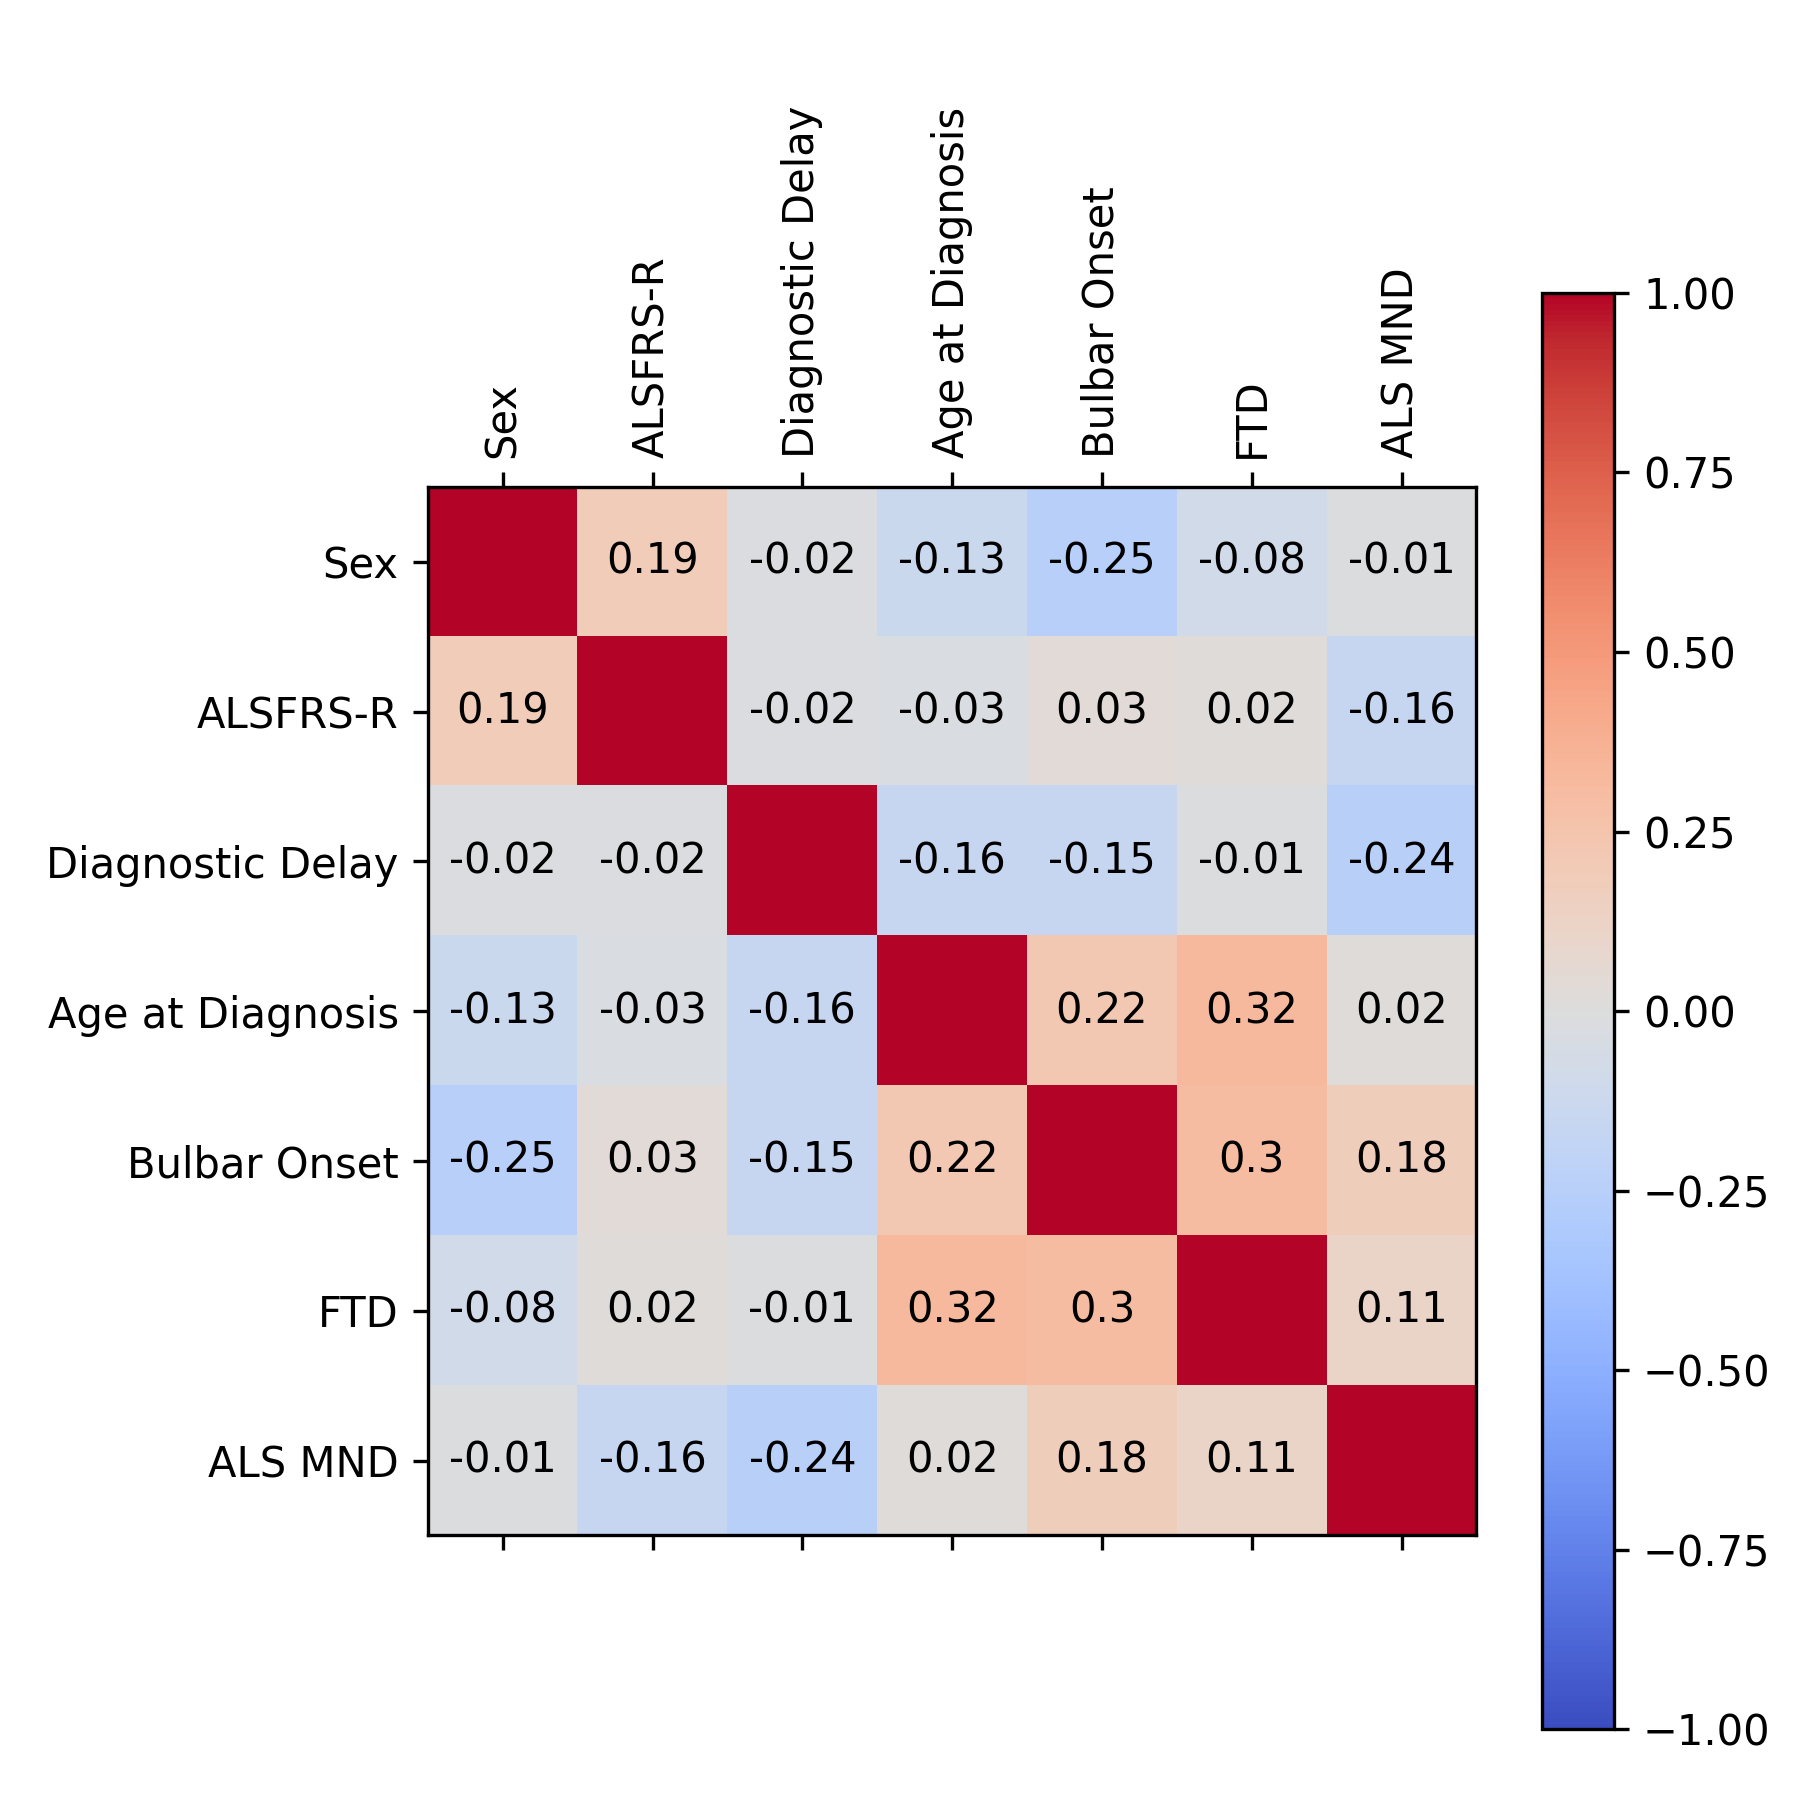
\includegraphics[width=0.75\linewidth]{figures/clinical_correlation}
    \caption[Correlations between the clinical variables of $n=125$ MND patients, as calculated by Pearson's correlation coefficient.]{Correlations between the clinical variables of $n=125$ MND patients, as calculated by Pearson's correlation coefficient. \textbf{Acronyms:} FTD = frontotemporal dementia, ALS = amyotrophic lateral sclerosis, ALSFRS-R = amyotrophic lateral sclerosis functional rating scale - revised.}
    \label{fig:clinicalcorrelation}
\end{figure}

%The multivariable models all resulted in broken proportional hazards assumptions, which were fixed by screening the input variables by their univariable significance.
%This approach is not without controversy, as it was possible that features that were not significant univariably could be significant in the multivariable model.
%However, we did not find this to be the case in our analysis, since the screened imaging and multimodal models resulted in more significant features than the unscreened models.
The multivariable models initially violated proportional hazards assumptions, rectified by screening input variables based on their univariable significance.
While this method may be controversial due to the potential significance of non-significant univariable features in multivariate models, our analysis found the screened imaging and multimodal models yielded more significant features than unscreened ones.

The multivariable imaging model revealed unexpected findings, including harmful effects associated with larger cerebral white matter and thalamus volumes.
In contrast, the univariable analysis showed protective effects of larger thalamus volume and no significant association with survival for larger cerebral white matter volume.
Additionally, previous studies indicated that thalamic atrophy suggested faster disease progression, though not necessarily linked to survival~\cite{sendaStructuralMRICorrelates2017,dieckmannCorticalSubcorticalGrey2022}.
High correlations among regional brain volumes exacerbated collinearity issues, potentially leading to unstable coefficient estimates and variable effects.
One approach to address collinearity is dimensionality reduction, such as principal component analysis (PCA), as employed by Westeneng and colleagues to group brain regions before survival analysis~\cite{westenengSubcorticalStructuresAmyotrophic2015}.
%
%The multivariable imaging model resulted in some clinically unintuitive results, such as reported significantly harmful effects of larger cerebral white matter volume and larger volume of the thalamus.
%In the univariable analysis, larger thalamus volume was significantly protective, and larger cerebral white matter volume was not significantly associated with survival.
%Moreover, previous work suggests that atrophy in the thalamus suggests faster disease progression, although this is not necessarily associated with survival~\cite{sendaStructuralMRICorrelates2017,dieckmannCorticalSubcorticalGrey2022}.
%The regional brain volumes are highly correlated, which increases collinearity in the model.
%Collinearity can lead to unstable estimates of the coefficients, and possibly explain a variable effect switching from harmful to protective or vice versa.
%
%One way to mitigate the effect of collinearity in the model is to use dimensionality reduction techniques, such as principal component analysis (PCA), to reduce the number of features in the model.
%Westeneng and colleagues used this technique to group the brain into larger regions based on their principal components before applying to a survival analysis model~\cite{westenengSubcorticalStructuresAmyotrophic2015}.

Diagnostic delay and FTD lost significance in the multivariable clinical model (both screened and unscreened) when age at diagnosis was included, possibly due to correlations among clinical features, shown in Figure~\ref{fig:clinicalcorrelation}.
%This lost significance could be explained by the correlations in the clinical features, shown in Figure~\ref{fig:clinicalcorrelation} as heatmap of Pearson's correlation coefficients.
For instance, age at diagnosis was strongly positively correlated with FTD, leading to its loss of significance in the presence of age at diagnosis, which remained significant.
Similarly, diagnostic delay, most negatively correlated with ALS MND, lost significance despite its univariable significance.


%In multivariable models, correlated features are less likely to be significant because their effect has already been accounted for by the significant features.
%Figure~\ref{fig:clinicalcorrelation} shows that age at diagnosis was the most positively correlated with FTD, which could explain why FTD lost significance in the clinical model when age at diagnosis was included, and age at diagnosis remained significant.
%Moreover, diagnostic delay is the most negatively correlated with ALS MND, which resulted in diagnostic delay losing significance, even though it was significant univariably.

%The presence of the amygdala in the final multimodal significant features was interesting, since brain regions which are more commonly associated with MND, such as the brain stem, were not significant.
%This could, again, be explained by the correlations between the features included in the model.
%Figure~\ref{fig:multimodalcorrelations} in the appendices showed that the most negative correlation between FTD and a brain region was with the amygdala (coefficient of -0.40), which could explain why FTD lost significance in the clinical model when the amygdala was included.
%Moreover, the brain stem was highly correlated with the amygdala (coefficient of 0.60), which could explain why the brain stem lost significance in the multimodal model, even though it was implicated in lower motor neuron degeneration in MND .

The presence of the amygdala in the final multimodal significant features was intriguing, as more typical MND-associated regions like the brain stem were not significant.
This observation might be attributed to correlations between features in the model, such as the strong negative correlation between FTD and the amygdala, and the high correlation between the amygdala and the brain stem, shown in Figure~\ref{fig:multimodalcorrelations} in the appendices.
Consequently, FTD lost significance when the amygdala was included, and the brain stem lost significance in the multivariable multimodal model despite its relevance to MND.

Another example of this was that the age at diagnosis was not significant in the multimodal model, even though it was significant in the clinical model.
Age at diagnosis was correlated with lateral ventricle volume (coefficient of 0.49), which could explain why age at diagnosis lost significance in the multimodal model when lateral ventricle volume was included.

The absence of these clinical variables in the imaging CPH may have led to the model picking up on brain structures indirectly related to survival, acting as markers for clinical features influencing survival.
For instance, older age at diagnosis and FTD, associated with brain atrophy, led to significant limbic structures: thalamus, amygdala, and caudate.
The multimodal CPH model addressed this by incorporating clinical features influencing survival.
However, high collinearity between brain volumes and clinical features could mean that individual volumes or clinical features were highlighted as significant, even if both influenced survival.

%The multimodal CPH mitigated the effect of the model picking up on brain structure not directly influencing survival, because we included the clinical features that are influencing survival into the model as well.
%However, the trade-off was that the collinearity was high, both within the brain volumes and also between the brain volumes and the clinical features, which could mean that individual volumes were picked out as significant over clinical features and vice versa, even if both were influencing survival.

Finally, the fit statistics in Table~\ref{tab:coxfitmetrics} show that the fit improved with multimodal features.
Although adding more features to a survival model is likely to increase its fit metrics, AIC also considers the number of features in the model in its calculation, so it can be concluded that the multimodal features added more information to the model than the clinical or imaging features alone.

%\begin{itemize}
%    \item It could also be that the model is picking up on brain structure not directly influencing survival, but markers of clinical features that are influencing survival, such as older age at diagnosis, which is associated with brain atrophy, and FTD, which is associated with limbic atrophy.
%    \item Interesting that limbic structures were being picked up as significant: thalamus, amygdala, and caudate. This could be because they are involved with cognitive and behavioural changes, which is a significant factor in MND survival, and was shown to be significant univariably with co-presence of FTD.
%\end{itemize}
%
%This correlation-driven loss of significance was also seen in the multimodal models.
%\begin{itemize}
%    \item Combining the clinical and imaging measures into one model should mitigate the effect of the model picking up on brain structure not directly influencing survival, because we will be including the clinical features that are influencing survival into the model as well
%%    \item Remaining clinical features are consistent with literature, but age at diagnosis was no longer significant.
%%    \item A marker of an aging brain is general atrophy, which can be shown by larger lateral ventricles, so it's possible that the model is picking up on the same information from the brain structure as it is from the age at diagnosis, because the lateral ventricles are significant in the multimodal model.
%%    \item Inspecting the correlations between the features found that age at diagnosis is correlated with lateral ventricle volume (coefficient of 0.49).
%%    \item Moreover, FTD has the most negative correlation with amygdala out of all the brain regions (coefficient of -0.40), which could explain why FTD lost significance in the clinical model when amygdala was included.
%%    \item Surprising that the brain stem is not significant in the multimodal model, because it is often implicated in MND survival but it has high correlation with the amygdala (0.6) so this is likely why it lost significance.
%    \item Fit statistics: fit improved with multimodal features - this could be just because we're adding more features, but it could also be because we're adding more information. AIC takes number of features into account, so it's not just that we're adding more features in the multimodal model.
%\end{itemize}
\subsection{Limitations}
The counter-intuitive results in the imaging multivariable model were likely due to limitations in this analysis.
Firstly, the sample size was relatively small ($n=125$), which could mean that the results were due to cohort-specific factors.
Moreover, the data came from two studies and multiple sites without harmonisation to account for site-specific factors.
However, omitting site-specific factors could eliminate important disease-related information.
Further investigation into the impact of sites on the results, such as incorporating site as a variable in the model, could provide insights.

Secondly, the scans were not consistently conducted at the time of diagnosis, potentially affecting the representativeness of brain volumes concerning the clinical features.
Given the rapid progression of MND, the allowance of a 12-month window around diagnosis for scan inclusion is wide. However, this compromise between sample size and data quality was necessary for this analysis.
In the future, we aim to increase the sample size, which would allow us to look at scans taken closer to diagnosis.

The collinearity of the brain volumes introduced instability into the model.
The summing of the left and right regions was done to mitigate this, but this could have also introduced information loss if the left and right regions were not equally important to survival.
Future work to mitigate this further would be to implement dimensionality reduction techniques before inputting the brain volumes into the model.

Finally, the univariable screening of the features could have introduced bias into the model, as features that are not significant univariably could have been significant in the multivariable model.
Although we did not find this to be the case, there are other ways to attempt to fix the proportional hazards assumption, such as using time-dependent covariates or stratifying the model by a variable, and there are other ways to screen the features, such as using a LASSO regression to select the most important features.

%Take home message:
%\begin{itemize}
%    \item Using imaging-derived feature with clinical features increases concordance, more information into the model is better, makes the clinical measure significant as well when it wasn't before
%    \item Would this result also be sustained when using more sophisticated machine learning models? Instinct says yes because they can handle more features and more complex relationships between features - perhaps collinearity of the brain volumes would not be such an issue
%\end{itemize}

\section{Conclusion}

In this chapter, we have shown that both brain region volumes and clinical features were significantly associated with survival in MND, and that including both data modalities in a survival model increased the quality of the model's fit to the data.
The clinical features that were significantly associated with survival were consistent with the existing literature, but some of the imaging features were not, until the incorporation of clinical features.
This suggests that incorporating imaging-derived features with clinical features was a valuable approach to survival analysis in MND, and that the multimodal model was more informative than the clinical or imaging models alone.

The issues encountered during the analysis were likely due to the collinearity of the brain volumes and the correlations between the brain volumes and the clinical features.
Future work will aim to address these issues by extending this analysis to include dimensionality reduction and improved clinical characterisation of the patients, as well as increased sample size.
\chapter{Fusilli: Developing a Data Fusion Python Library}
\label{fusilli_development}

The previous chapter explored multimodal data in a relatively simple setting of a survival analysis model.
In the field of machine learning, multimodal data can be integrated as it was in the Cox model, by concatenating the data before inputting it into the model, or by using more complex methods that aim to capture the potentially non-linear relationships between the modalities.
These techniques fall under the umbrella of multimodal data fusion.

This chapter discusses multimodal data fusion in more detail and describes the development of Fusilli, a Python package for multimodal data fusion experimentation and analysis.

\section{Introduction}

Multimodal data fusion is the process of combining data from different sources to make predictions or decisions, often through the use of deep learning.
The goal of combining different modalities is to improve the performance of a model by leveraging the relevant information from each modality and fusing them in a way that improves the model's performance.
There are many research fields where multimodal data fusion is used, such as in agriculture to predict crop yields and detect diseases~\cite{s.s.gopiMultimodalMachineLearning2023, patilRiceFusionMultimodalityData2022}, in disaster management to analyse response scenarios from audio and social media posts~\cite{algiriyageMultisourceMultimodalData2021}, and in robotics to help direct the robots with multiple sensors~\cite{duanMultimodalSensorsMLBased2022}.
Moreover, the types of models used in multimodal data fusion can vary widely, from geometric deep learning to relatively simple neural network architectures~\cite{cuiDeepMultimodalFusion2022}.

%In the context of my PhD, I am investigating multimodal data fusion for MND prognosis prediction.
%There has been minimal research on deep learning for prognosis prediction in MND~\cite{pancottiDeepLearningMethods2022, mullerExplainableModelsDisease2021}, and only one model created for deep-learning based multimodal data fusion~\cite{vanderburghDeepLearningPredictions2017}.
%However, there are many data fusion models that have been used in other fields that could be directly applicable to MND .
%There have been systematic reviews on the topic of data fusion that compare models, but only qualitatively~\cite{cuiDeepMultimodalFusion2022, gaoSurveyDeepLearning2020, stahlschmidtMultimodalDeepLearning2022, yanDeepMultiviewLearning2021}.
%Therefore, with limited knowledge from literature on the best models for MND data, it is important to experiment with a wide variety of models to find the best one for the task.

My PhD investigates predicting MND prognosis, an area with minimal deep learning research~\cite{pancottiDeepLearningMethods2022, mullerExplainableModelsDisease2021} and only one model specially created for deep-learning based multimodal data fusion~\cite{vanderburghDeepLearningPredictions2017}.
Despite systematic reviews on multimodal data fusion attempting qualitative comparison between models in many areas of applications~\cite{cuiDeepMultimodalFusion2022, gaoSurveyDeepLearning2020, stahlschmidtMultimodalDeepLearning2022, yanDeepMultiviewLearning2021}, a lack of quantitative comparison necessitates experimentation with many models from other fields to identify the most effective for MND prognosis prediction.

%Obtaining this wide variety of models to experiment with, however, is not a straightforward process for a number of reasons.
%Firstly, the terminology used to describe what I have chosen to call ''multimodal data fusion'' varies widely, with terms such as but not limited to multi-view, cross-heterogeneous, multi-source, and integrated learning.
%Secondly, the studies that introduce these models often do not include code for the reader to run the model.
%Morever, when code is included, it is often written in different languages, with varying guidance, quality, and maintenance.
Acquiring a diverse range of models for experimentation is made difficult by the use of inconsistent terminology and the common unavailability of maintained, quality code provided alongside studies.

A way to address these problems is to create a curated collection of models for somebody interested in multimodal data fusion to consult.
As far as I am aware, there are three Python packages that house collections of deep learning based data fusion models: ``Multi-view-AE''~\cite{aguilaMultiviewAEPythonPackage2023}, ``CCA-Zoo''~\cite{chapmanCCAZooCollectionRegularized2021}, and ``pytorch-widedeep''~\cite{zaurinPytorchwidedeepFlexiblePackage2023}.
However, each of these packages only includes models with specific frameworks (autoencoders, CCA, and Google's ``wide and deep'' models, respectively), which limits the variety of models available for comparison.

Therefore, I aimed to develop a Python package for training and comparing multimodal data fusion models with any architecture.
This Python package is named Fusilli, as a portmanteau of ``fuse easily''.
Fusilli works by taking the user's multimodal data and training it on a variety of models, and then comparing the models' performances.

\section{Development and Implementation}

\subsection{Software Design Choices}

Before developing Fusilli, the following design goals were set to ensure the package would be useful for a wide range of users and tasks, as well as for my research.
\vspace{0.3cm}

\noindent\textbf{Modularity}: Fusilli should be modular, meaning that the various functionalities within the package should be independent of each other.
This would allow for easy addition of new models in the future and easy adjustments to the package's functionality.
Testing, which is the process of writing code to check that the package works as expected, would also be easier with a modular design, and so the package would be more reliable.

\vspace{0.3cm}

\noindent\textbf{Beginner-friendly and expert-friendly}:  Fusilli should be beginner-friendly, with users able to compare the different models without needing expertise in deep learning or Python programming.
This would make it different from other similar packages, which require the user to set up their own experiments.
On the other hand, Fusilli should also be expert-friendly, with users who are more capable of being able to change the training parameters, modify the models, and access the trained models for further experiments.

\vspace{0.3cm}

\noindent\textbf{Wide applicability}:
Fusilli should include a wide variety of models, to ensure that the best model for a given task can be found.
Moreover, this would ensure that the package is useful for a wide range of users, as different users may have different requirements for model architectures based on their tasks and data.

\vspace{0.3cm}

\noindent\textbf{Support for two modalities}: The models in Fusilli will support data fusion between either two types of tabular data (e.g. clinical data and brain region volumes data) or between an image and tabular data (e.g. MRI images and clinical data).
For wide applicability, Fusilli should be able to handle two-dimensional and three-dimensional images and tabular data of any size.

\vspace{0.3cm}

\noindent\textbf{Support for different prediction tasks}: The prediction tasks that Fusilli should support are regression and classification.
From the literature, these are the most common tasks for multimodal data fusion and are the tasks that I am interested in for my research.


\subsection{Implementation}

Fusilli was implemented in Python, using the PyTorch and PyTorch Lightning libraries for deep learning.
PyTorch is a popular library for deep learning, and is known for its flexibility and ease of use.

\noindent For a user to apply Fusilli to their own problem, they must specify:
\begin{itemize}
  \setlength\itemsep{-0.5em}
    \item \textbf{Data}: The user's data, which must be in the form of a .csv file for tabular data, and .pt files for images.
    \item \textbf{Task}: The task that the user wants to perform, which can be either regression or classification (binary or multiclass).
    \item \textbf{Models}: The models that the user wants to compare, which can be any of the models included in Fusilli.
    \item \textbf{Output}: The output directory for the trained models and the results of the experiments.
\end{itemize}

\noindent The user can also specify experiment specifics, which are set to default values if not specified.
Examples of experiment specifics include the training and validation data splits, the maximum number of epochs to train for, and the batch size.
The user can also modify model hyperparameters and architectures.

After the user has specified these, the user calls two functions in Fusilli to train the models:
\begin{itemize}
\setlength\itemsep{-0.5em}
    \item \texttt{prepare\_fusion\_data()}: This function prepares the data for training, including splitting it into training and validation sets and running any model-specific data preparation steps.
    \item \texttt{train\_and\_save\_models()}: This function trains the models on the user's data, and outputs the trained models.
\end{itemize}

Finally, the user can call functions to evaluate a single model or compare the models, which will output the performance of the models on the user's validation data or external test data.
The evaluation figures are saved in the output directory, and the user can also access the trained models for further analysis.

\subsection{Fusion Methods}

A literature search was conducted to find models that could be included in Fusilli.
The search criteria aimed to return papers that mentioned machine learning, multimodality, and image and tabular data, with variants of these terms used to capture a wide range of papers.
The resulting papers were checked for relevance and papers were discarded which use the same model as another paper, which happened frequently.

The models were categorised based on the taxonomy defined by Cui and colleagues in their review of data fusion methods for diagnosis and prognosis~\cite{cuiDeepMultimodalFusion2022}.
Figure~\ref{fig:fusilli_taxonomy} is a diagram taken from the review, which shows the general architecture differences between the categories, and Table~\ref{tab:fusilli_taxonomy} includes descriptions of the categories.

\begin{table}
    \centering
    \caption[Descriptions of data fusion model categories used in Fusilli.]{Descriptions of data fusion model categories used in Fusilli, first proposed by Cui and colleagues~\cite{cuiDeepMultimodalFusion2022}.}
    \label{tab:fusilli_taxonomy}
    \begin{tabular}{|p{0.25\textwidth}p{0.7\textwidth}|}
        \hline
        \textbf{Category} & \textbf{Description} \\ \hline
        \textbf{Operation-based} & Models that fuse data based on operations such as concatenation, addition, or multiplication. This can be done at any point in the model, such as at the input, hidden layers, or output. \\ \hline
        \textbf{Attention-based} & Models that use attention mechanisms to weight the importance of different modalities. \\ \hline
        \textbf{Graph-based} & Models with a graph structure, such as graph convolutional networks, which capture the relationships between the data by treating them as nodes in a graph with edges connecting them representing the relationships. \\ \hline
        \textbf{Subspace-based} & Models that project the data into a joint lower-dimensional space, for example with deep learning methods such as autoencoders. \\ \hline
        \textbf{Tensor-based} & Models that use tensor operations to fuse the data to capture inter- and intra-modality correlations. \\ \hline
    \end{tabular}
\end{table}

%\begin{itemize}
%\setlength\itemsep{-0.5em}
%    \item \textbf{Operation-based}: Models that fuse data based on operations such as concatenation, addition, or multiplication.
%    This can be done at any point in the model, such as at the input, hidden layers, or output.
%    \item \textbf{Attention-based}: Models that use attention mechanisms to weight the importance of different modalities.
%    \item \textbf{Graph-based}: Models with a graph structure, such as graph convolutional networks.
%    \item \textbf{Subspace-based}: Models that project the data into a joint lower-dimensional space, possibly with deep learning methods such as autoencoders.
%    \item \textbf{Tensor-based}: Models that use tensor operations to fuse the data to capture inter- and intra-modality correlations.
%\end{itemize}

\begin{figure}
    \centering
    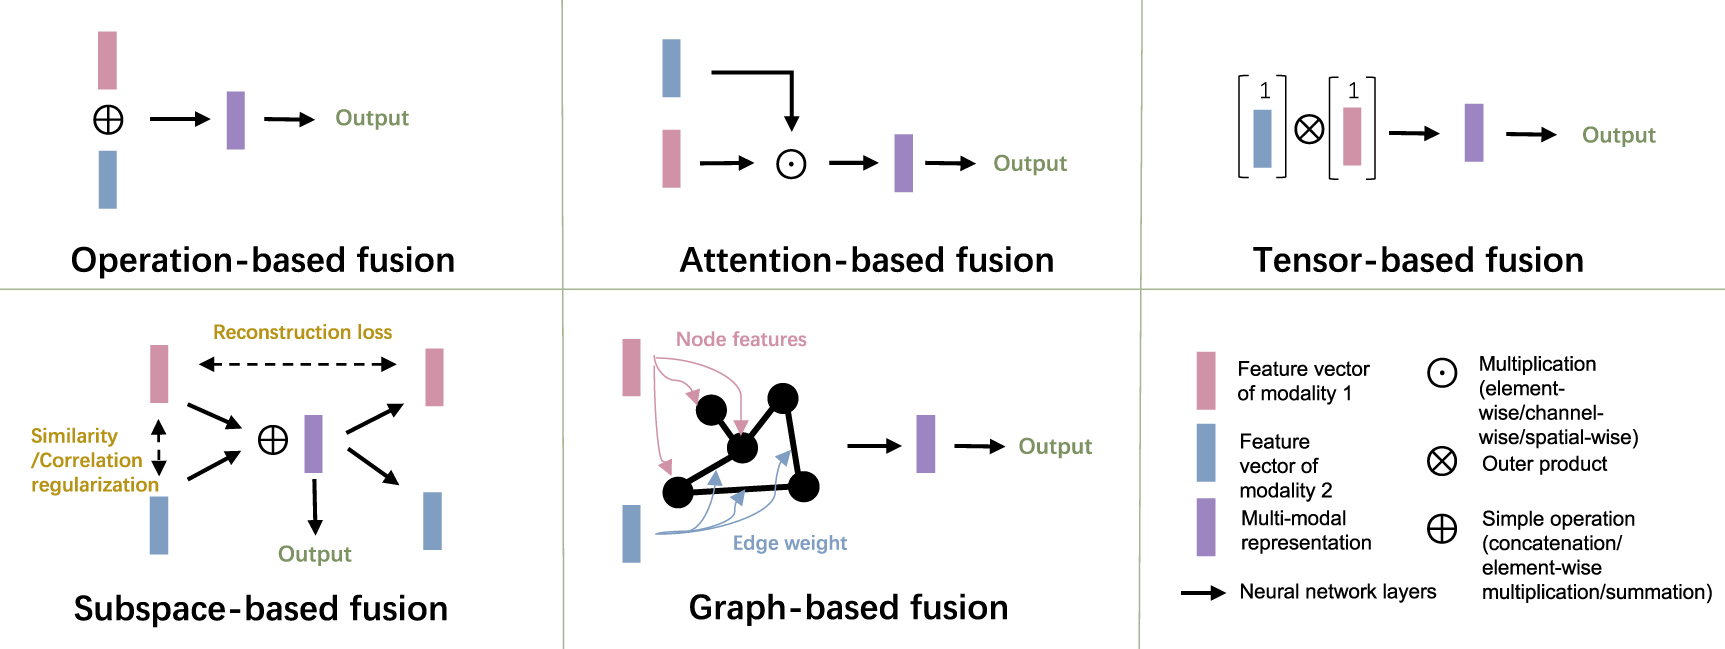
\includegraphics[width=\textwidth]{figures/cui_diagram}
    \caption[Diagrams of the categories of the multimodal fusion models in Fusilli.]{Cui and colleagues' diagram of the architecture-based taxonomy of multimodal data fusion models used in Fusilli~\cite{cuiDeepMultimodalFusion2022}.}
    \label{fig:fusilli_taxonomy}
\end{figure}

%Figure~\ref{fig:fusilli_taxonomy} shows the architecture-based taxonomy of multimodal data fusion models, taken from Cui et al.~\cite{cuiDeepMultimodalFusion2022}.

Another common categorisation is ''early'', ''intermediate'', and ''late'' fusion, which refers to the point in the model where the data is fused.
However, this categorisation is too simplistic for the variety of model architectures in Fusilli, and so the architecture-based taxonomy was chosen.

\begin{table}[!ht]
    \caption[The models included in Fusilli $v1.2.3$, categorised by their fusion method and modalities.]{The models included in Fusilli $v1.2.3$, categorised by their fusion method and modalities.
    References are included where applicable. The Fusilli implementation is not a direct copy of the referenced model, and may have been modified to fit the package's requirements.
    \textbf{Acronyms}: GNN = Graph Neural Network, MCVAE = Multi-Channel Variational Autoencoder.}
    \label{tab:fusillimodelslist}
    \centering
    \begin{tabular}{|p{8cm}ll|}
        \hline
        \textbf{Model name (and reference where applicable)} & \textbf{Fusion} & \textbf{Modalities} \\ \hline
        Tabular1 uni-modal & Unimodal & Tabular Only \\ \hline
        Tabular2 uni-modal & Unimodal & Tabular Only \\ \hline
        Image unimodal & Unimodal & Image Only \\ \hline
        Activation function map fusion~\cite{chenMDFNetApplicationMultimodal2023} & Operation & Tabular-tabular \\ \hline
        Activation function and tabular self-attention~\cite{chenMDFNetApplicationMultimodal2023} & Operation & Tabular-tabular \\ \hline
        Concatenating tabular data & Operation & Tabular-tabular \\ \hline 
        Concatenating tabular feature maps~\cite{gaoReducingUncertaintyCancer2022} & Operation & Tabular-tabular \\ \hline
        Tabular decision & Operation & Tabular-tabular \\ \hline 
        Channel-wise multiplication net (tabular)~\cite{duanmuPredictionPathologicalComplete2020}  & Attention & Tabular-tabular \\ \hline
        Tabular Crossmodal multi-head attention~\cite{golovanevskyMultimodalAttentionbasedDeep2022}  & Attention & Tabular-tabular \\ \hline
        Attention-weighted GNN~\cite{bintsiMultimodalBrainAge2023} & Graph & Tabular-tabular \\ \hline
        Edge Correlation GNN & Graph & Tabular-tabular \\ \hline 
        MCVAE Tabular~\cite{antelmiSparseMultiChannelVariational2019}  & Subspace & Tabular-tabular \\ \hline
        Concatenating tabular data with image feature maps~\cite{liFusingMetadataDermoscopy2020}  & Operation & Tabular-image \\ \hline
        Concatenating tabular and image feature maps~\cite{gaoReducingUncertaintyCancer2022} & Operation & Tabular-image \\ \hline
        Image decision fusion & Operation & Tabular-image \\ \hline 
        Channel-wise Image attention~\cite{duanmuPredictionPathologicalComplete2020} & Attention & Tabular-image \\ \hline
        Crossmodal multi-head attention~\cite{golovanevskyMultimodalAttentionbasedDeep2022} & Attention & Tabular-image \\ \hline
        Trained Together Latent Image + Tabular Data~\cite{zhaoMultimodalDeepLearning2022} & Subspace & Tabular-image \\ \hline
        Pretrained Latent Image + Tabular Data~\cite{zhaoMultimodalDeepLearning2022} & Subspace & Tabular-image \\ \hline
        Denoising tabular autoencoder with image maps~\cite{yanRicherFusionNetwork2021} & Subspace & Tabular-image \\ \hline
    \end{tabular}
\end{table}

More models were found in the literature than were included in Fusilli due to the time constraints of the project, but the models included in Fusilli were chosen based on their popularity, availability of code, and the variety of architectures they represent.
Moreover, unimodal benchmarks were included in Fusilli to allow for comparison between the multimodal models and unimodal models.
Table~\ref{tab:fusillimodelslist} shows the models implemented in Fusilli, along with their fusion categories and references.



\section{Results}

Fusilli version 1.0.0 was published on 30th November 2023 and has since been updated to version 1.2.3~\cite{townendFlorencejtFusilliFusilli2024}.
Currently, Fusilli is under review for publication in the Journal of Open Source Software (JOSS).
The package has been well-received on GitHub, having been favourited by 142 users and specially cloned by 12 users for their own modifications.
Moreover, I wrote an article on Medium about Fusilli, which has been read by 257 people, and two articles have been written about Fusilli by other people.

Fusilli is documented using Sphinx, a Python documentation generator.
Figure~\ref{fig:fusillidocs} shows an overview of the documentation, which includes tutorials for getting started, guidance for more advanced users, example Python scripts which run the models on simple data, a guide for people to contribute their own models, and the source code documentations.
The page ''Fusion Model Explanations'', partly shown in Figure~\ref{fig:fusillidocs}B, has a diagram and a text explanation for each model in Fusilli, which is useful for users to understand and compare the models' architectures with a standardised diagram style.

\begin{figure}
    \centering
    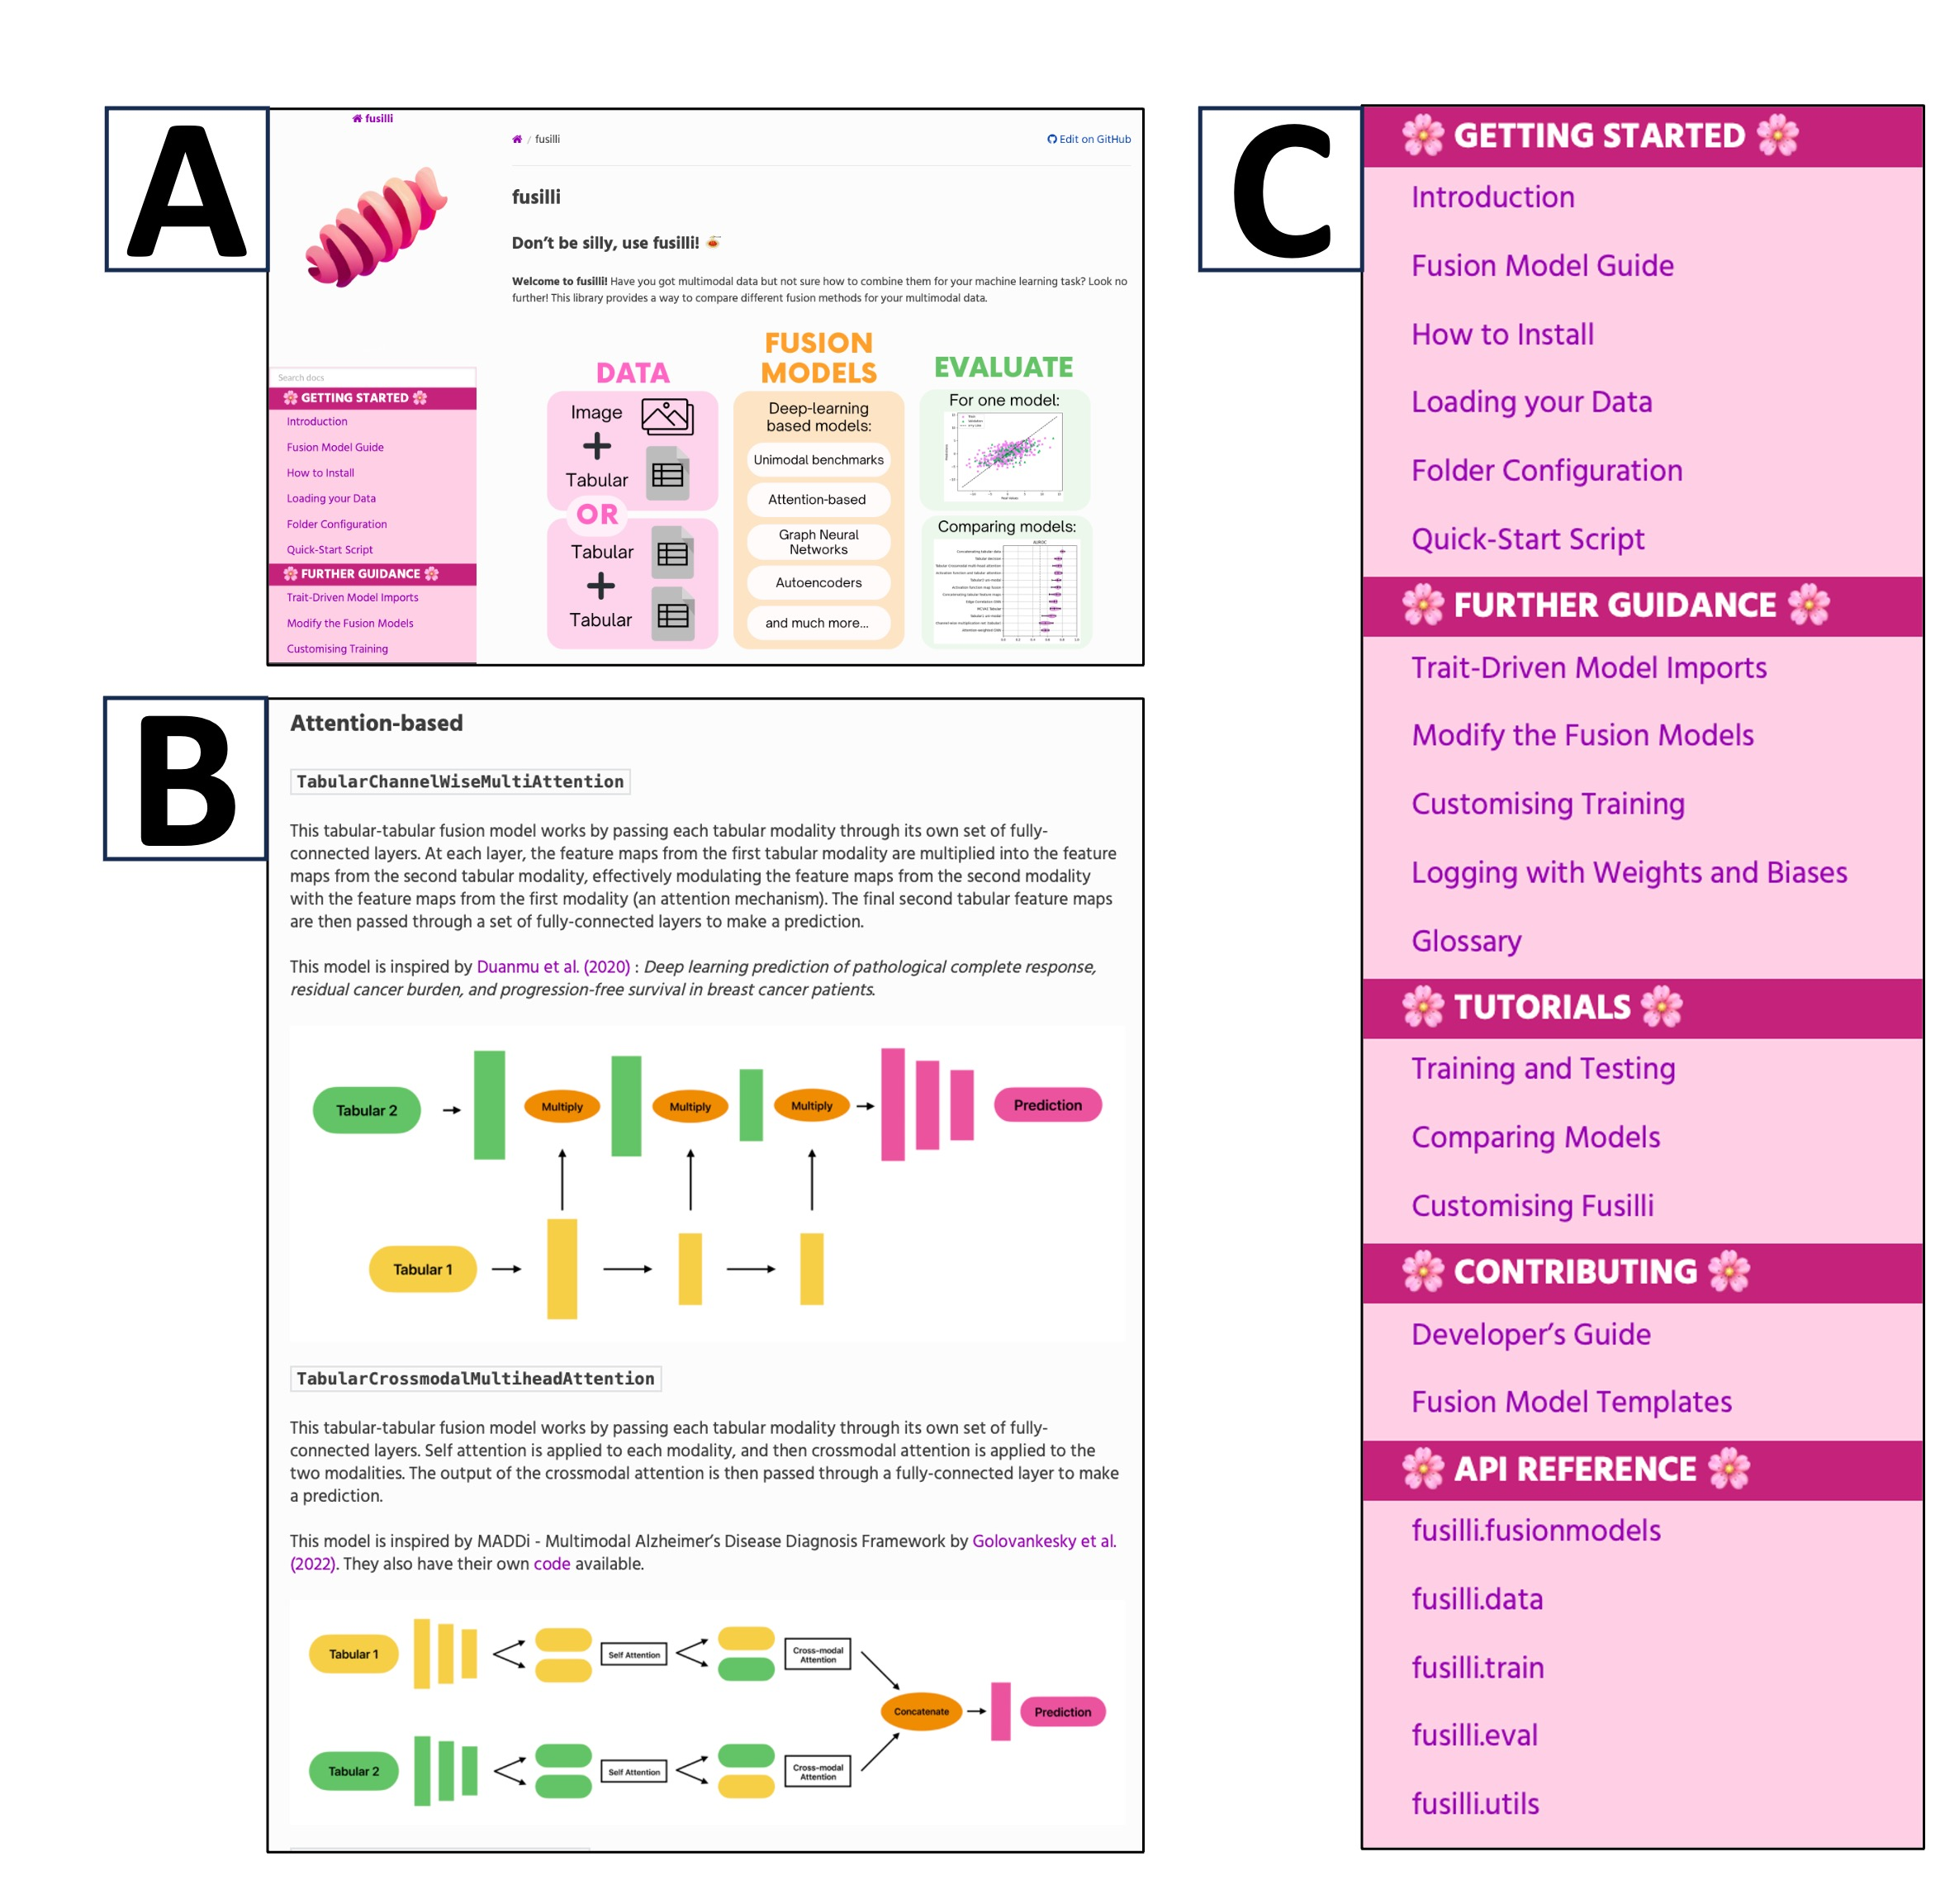
\includegraphics[width=1\linewidth]{figures/fusilli_documentation}
    \caption[Overview of the Fusilli documentation.]{Overview of the Fusilli documentation. \\
    \textbf{A}: The home page of the documentation, showing the logo and the diagram explaining Fusilli's purpose.\\
    \textbf{B}: Two examples of the fusion model explanations, complete with diagram and description with reference to the source paper, where applicable. \\
    \textbf{C}: The sidebar of the Fusilli documentation showing all the pages available, categorised into pages on getting started, further guidance for advanced users, tutorials on how to use Fusilli, guidance on contributing and templates for adding models, and the API references with explanations of the source code.
    }
    \label{fig:fusillidocs}
\end{figure}

Figures~\ref{fig:fusillioutputs}A, B, and C show the figures output by Fusilli after training, validating, and comparing the models respectively.
The format of the figures depends on the prediction task and the type of training used, with the figures shown being for a binary classification task with 5-fold cross-validation training.
If the user chooses to use train-test split training, the comparison figure is a bar chart instead of a violin plot.
Additionally, if the user trains a regression model, the performance evaluation will be a scatter plot of the predicted values against the true values.


\begin{figure}
    \centering
    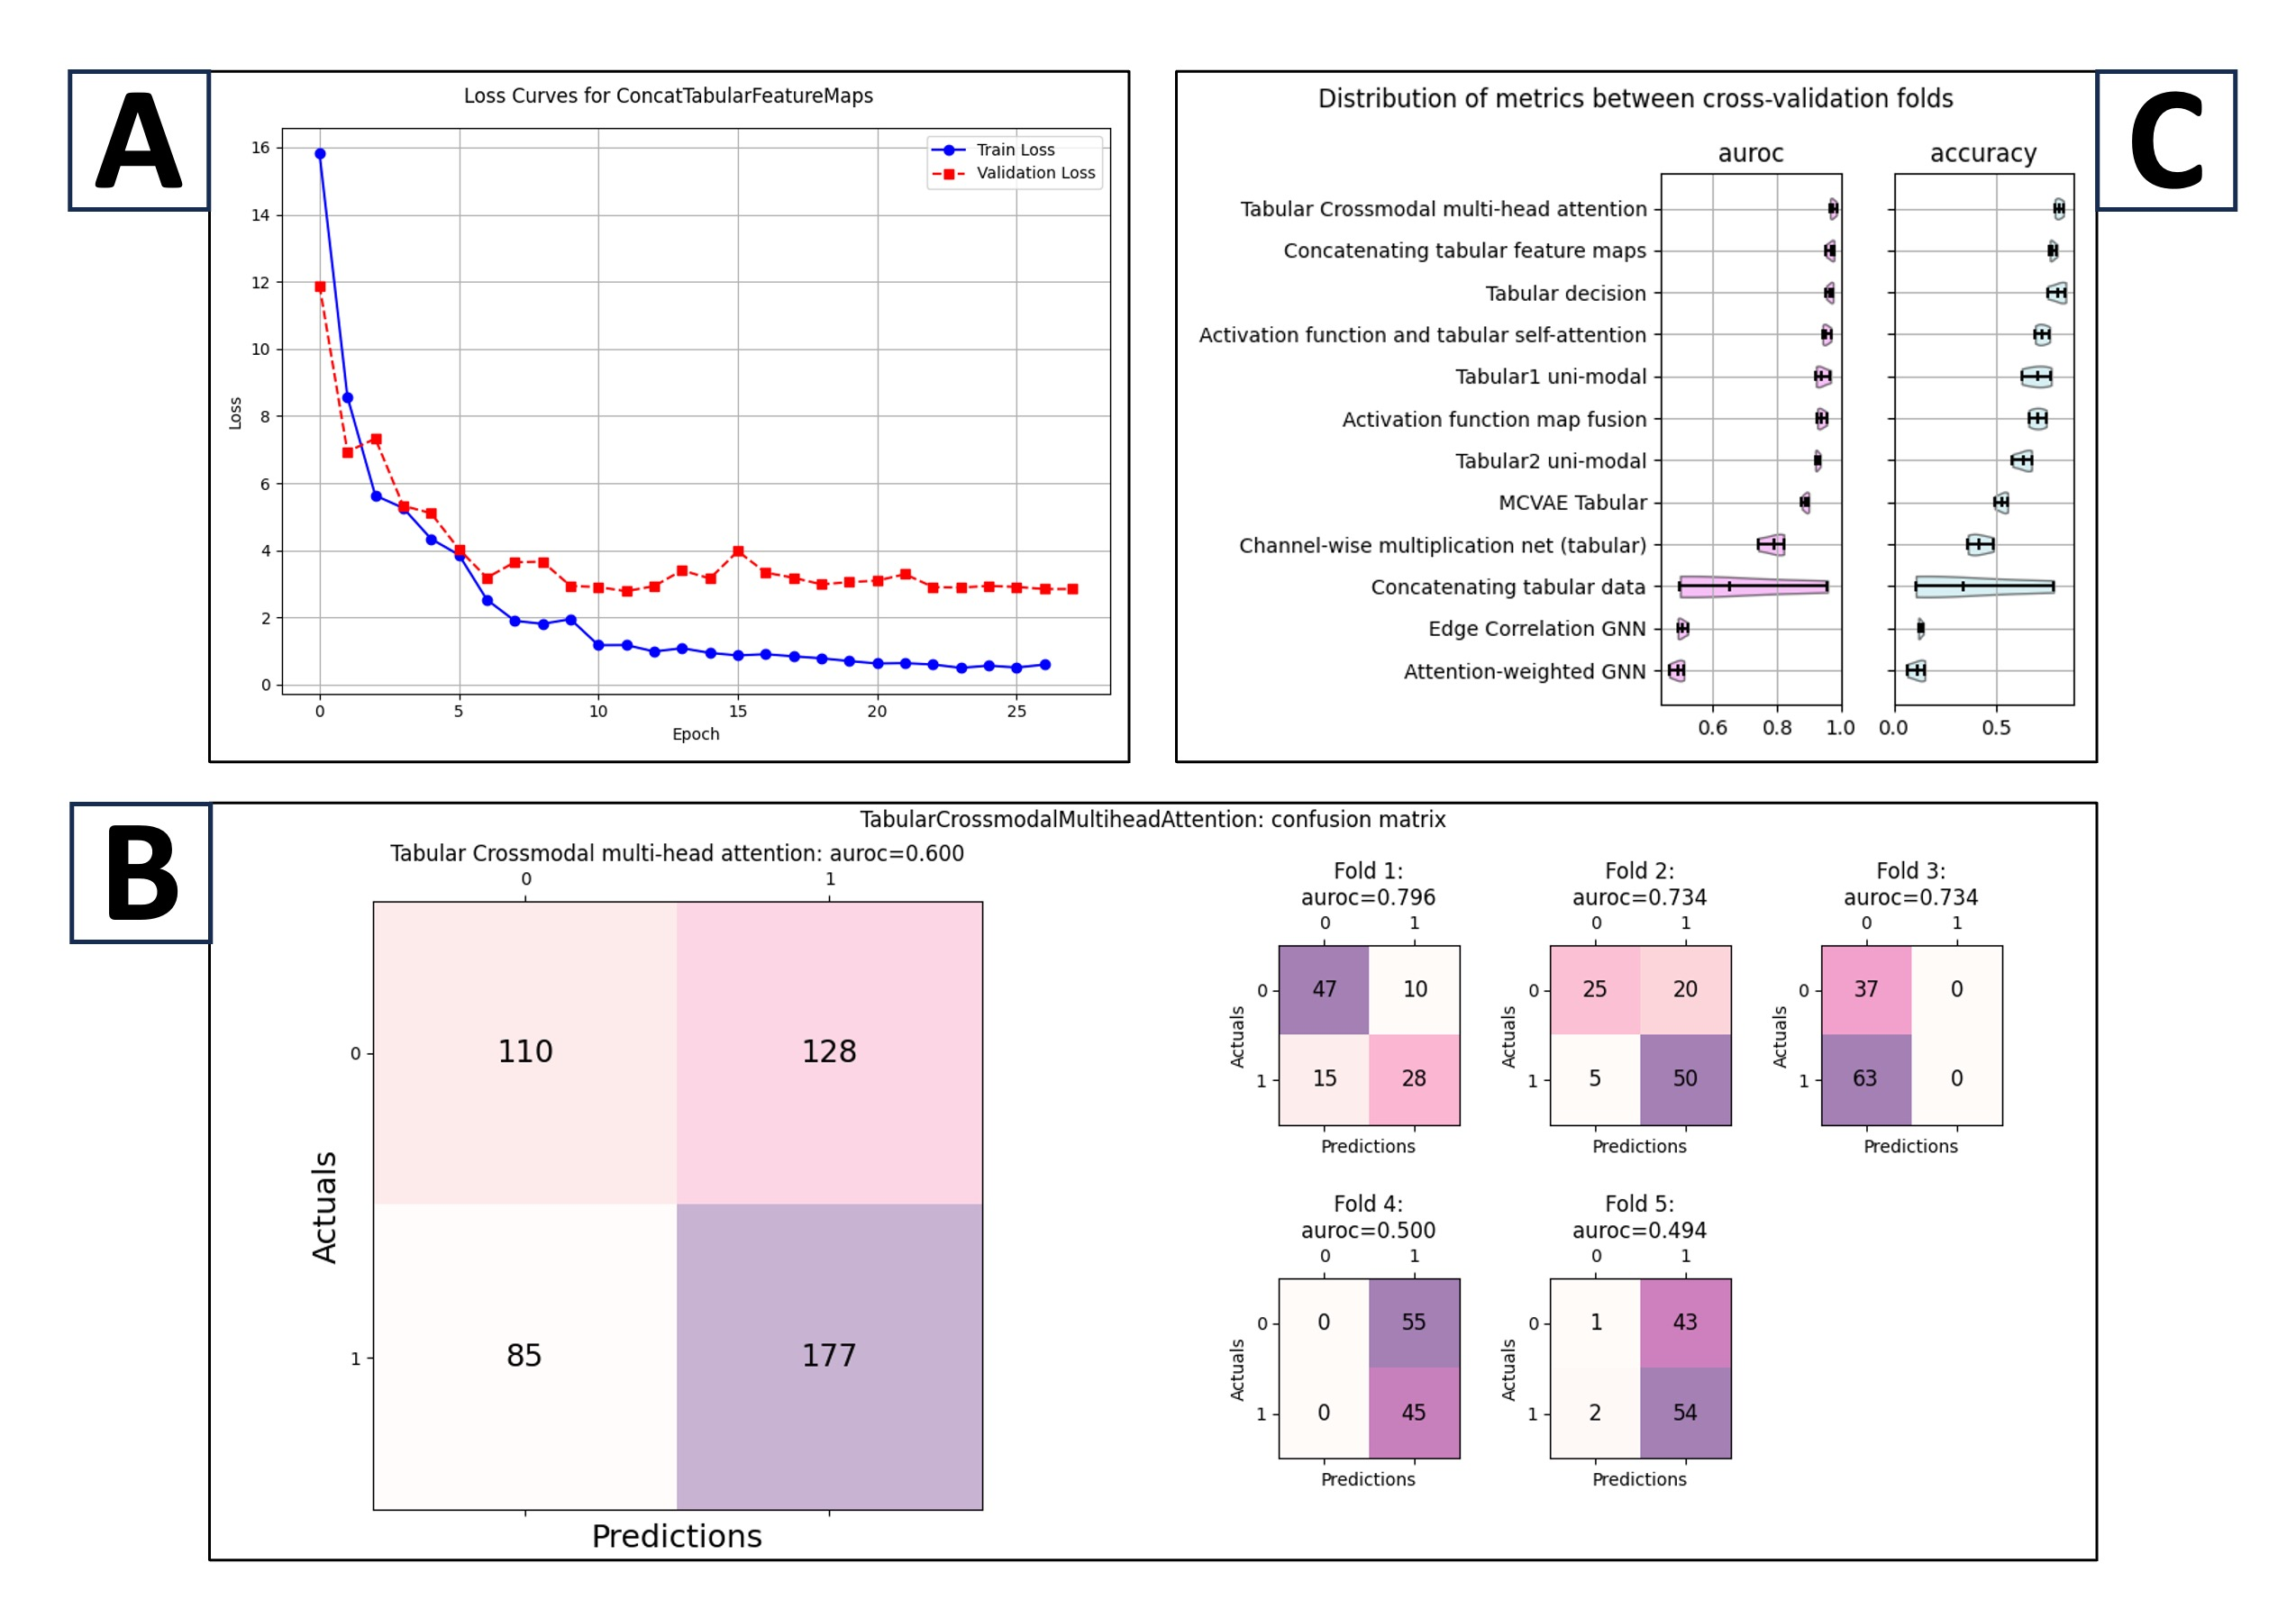
\includegraphics[width=1\linewidth]{figures/fusilli_outputs}
    \caption[Fusion model training, evaluation, and comparison figures output by Fusilli.]{Fusion model training, evaluation, and comparison figures output by Fusilli. \\
    \textbf{A}: The training and validation loss curves for an individual model.\\
    \textbf{B}: Performance evaluation of a model which was trained on a binary task with 5-fold cross validation. Both the validation performances of each fold and the overall performance from the aggregated folds are shown. \\
    \textbf{C}: Comparison of the models' performances on the validation data. The violin plot distributions are the distributions of the fold performances when using k-fold cross validation. If train-test split training is used, the comparison figure is a bar chart.
    }
    \label{fig:fusillioutputs}
\end{figure}


\section{Discussion}

Overall, Fusilli achieved the goals set out at the beginning of the project.
It has had interest from both beginners and experts, and there has been interest from people in different fields, such as thermal imaging.
Additionally, a hackathon project was run during the 2023 Centre for Medical Imaging Hackathon, where participants aimed to add new models to Fusilli, which was a success with two new models being added and more in development.

Fusilli has several limitations, most of which I hope to address with future updates to the software.
Firstly, Fusilli only supports two modalities, which is a limitation for tasks that may benefit from more than two modalities.
For example, in the context of MND prognosis prediction, using different types of MRI images (e.g. T1-weighted, T2-weighted, diffusion tensor imaging) could be beneficial, but Fusilli currently only supports one type of image alongside clinical information.
Moreover, Fusilli only supports inputting image data in the form of PyTorch .pt files, which requires the user to do some pre-processing of their data.
This is a limitation for users who may not be comfortable with Python, and would prefer to input their data in the form of JPEGs or NiFTI files, for example.
Fusilli also only supports regression and classification tasks, and does not support other tasks such as time-to-event analysis.
Finally, although the models included in Fusilli are popular and cover a wide variety of architectures, many more models in the literature could be included in Fusilli, and I hope to add these.

\section{Conclusion}
% Link to using fusilli on MND
In conclusion, Fusilli is a Python package for multimodal data fusion experimentation and analysis, specifically tackling the problem of lack of ways to compare models and lack of standardisation in the field.
I specifically made it for my PhD in fusing different data modalities in MND prognosis prediction.
The next chapter will discuss the application of Fusilli to MND prognosis prediction using the fusion of clinical information and brain region volumes.
% \begin{itemize}
%     \item Fusilli is a Python package for multimodal data fusion experimentation and analysis, specifically tackling the problem of lack of ways to compare models and lack of standardisation in the field.
%     \item I specifically made it for my PhD in fusing different data modalities in MND prognosis prediction
%     \item Link to next chapter on PPMI, ADNI, MIMIC: data fusion can be applied to any task where there are multiple data modalities describing one thing
%     \item Before going into MND, is there a clear benefit to different types of multimodal data fusion? Is there a consensus on the best approaches for different tasks?
%     \item MND sample size is small so we want to make sure we're using the best models by testing them on larger datasets with different applications
% \end{itemize}

\chapter{Fusilli on Open Data}
\label{fusilli_on_open_data}

\section{Introduction}
\begin{itemize}
    \item We've made Fusilli
    \item Testing the hypothesis that:
    \begin{itemize}
        \item Different tasks require different multimodal data fusion methods
        \item Fusilli is useful for selecting the best model
    \end{itemize}
    \item Why would multimodal data fusion be useful in specific healthcare tasks?
    \begin{itemize}
        \item Multifactorial diseases require multiple data types
        \item Data is expensive to collect
        \item We want to use all the data we have
    \end{itemize}
    \item Examples of data fusion in healthcare
    \begin{itemize}
        \item Oncology
        \item Etc
    \end{itemize}
\end{itemize}

\section{Data}
\subsection{ADNI}
\subsection{PPMI}
\subsection{MIMIC-IV and MIMIC-CXR}

\section{Methods}
\begin{itemize}
    \item Experiment details: different for each dataset
\end{itemize}

\section{Results}

\section{Discussion}

\section{Conclusion}
\begin{itemize}
    \item Now we know it's important/not important to use multimodal data fusion and to compare models
    \item Let's do it on MND data
\end{itemize}

\chapter{Fusilli on MND}
\label{fusilli_on_mnd}

\section{Introduction}
Only one deep learning model has been used to predict survival in MND through clinical data and neuroimaging data~\cite{vanderburghDeepLearningPredictions2017}.
This lack of research in multimodal data fusion in MND makes it difficult to conclude whether multimodal data is useful in predicting survival in MND .
Additionally, we have shown that there are many different multimodal data fusion methods available.
In Chapter~\ref{fusilli_development}, we developed a package called Fusilli to compare the performance of different multimodal data fusion methods, approximately half of which are designed to combine two tabular modalities.
In this chapter, we will use Fusilli to compare the performance of different tabular-tabular multimodal data fusion methods on predicting survival in MND patients using clinical and imaging extracted features data.
The aims of this work are to, firstly, assess the effect of different data fusion model architectures on prognostic performance, and secondly, to assess the value of baseline clinical and neuroimaging data in MND prognosis prediction.

\section{Data}

The data used in this analysis is from two studies: University College London Queen's Square Institute of Neurology's ALS Biomarkers Study~\cite{UKMNDCSG} and Ospedale San Raffaele's MND cohort.
Both of these datasets contain clinical data from the diagnostic visit and brain MRI data.

For patients to be included in the analysis, they must have a diagnosis of MND and have an outcome of interest (death or tracheostomy).
In the ALS Biomarkers Study, the outcome of interest is death, whereas in the Ospedale San Raffaele's MND cohort, the outcome of interest is death or tracheostomy.
Unfortunately, the Ospedale San Raffaele's MND cohort does not specify the date of death, so we have assumed that the date of death is the date of tracheostomy.

Patients in this analysis must have non-missing data for age at diagnosis, sex, date of diagnosis, date of death, date of symptom onset, site of onset, and baseline ALSFRS-R .
Additionally, patients must have a T1-weighted or T2-weighted MRI within 12 months before or after their date of diagnosis.

The final dataset contains 110 MND patients.
The patients in the cohort were split into two groups based on the median survival time: short survival group (less than 24 months) and long survival group (more than 24 months).

\subsection{Clinical Data}

The clinical variables chosen to be included in the analysis are based on the variables used in the ENCALS model~\cite{westenengPrognosisPatientsAmyotrophic2018} described in Chapter~\ref{literature_review}.
El Escorial criteria and FVC were not included in the analysis as they were not available in the Ospedale San Raffaele's MND cohort.
Features with missing data after the inclusion criteria were applied were features of FTD and presence of C9orf72 mutation.
Where these features were missing, they were assumed to be negative.
Moreover, where the MND type was missing, it was assumed to be ALS, as it is the most common.

\begin{table}
    \centering
    \label{tab:clinical_demographics}
    \caption{Differences in clinical demographics between the long and short survival groups.}
    \begin{tabular}{|p{5cm}|llll|}
    \hline
                                                        & \textbf{Overall}     & \textbf{Short}        & \textbf{Long}         & \textbf{P-Value}   \\
    \hline
     n                                                  & 110         & 55         & 55          &           \\ \hline
     Sex (Male), n (\%)                                     & 52 (47.3)   & 27 (49.1)  & 25 (45.5)   & 0.849     \\ \hline
     Site of Onset (Bulbar), n (\%)                          & 31 (28.2)   & 20 (36.4)  & 11 (20.0)  & 0.090     \\\hline
     Frontotemporal Dementia, n (\%)                       & 32 (29.1)   & 24 (43.6)  & 8 (14.5)   & \textbf{0.002}     \\\hline
     C9orf72 Mutation, n (\%)                               & 7 (6.4)     & 2 (3.6)    & 5 (9.1)   & 0.438     \\\hline
     ALSFRSr, mean (SD)                                  & 37.5 (7.2)  & 36.3 (7.2) & 38.7 (7.0)  & 0.081     \\\hline
     MND Type (ALS), n (\%)                                & 96 (87.3)   & 51 (92.7)  & 45 (81.8)   & 0.153     \\\hline
     Diagnostic Delay (months), mean (SD)                 & 12.5 (12.0) & 10.0 (9.8) & 14.9 (13.4) & \textbf{0.031}     \\\hline
     Age at Diagnosis (years), mean (SD)                   & 63.2 (11.8) & 69.1 (9.1) & 57.3 (11.3) & \textbf{\ensuremath{<}0.001 }   \\\hline
     Rate of ALSFRSr decline (points/month), mean (SD)       & 1.4 (1.7)   & 2.0 (2.2)  & 0.9 (0.7)   & \textbf{0.001}     \\\hline
     Survival (months), mean (SD)                         & 29.3 (23.2) & 12.3 (6.4) & 46.4 (21.3) & \ensuremath{<}0.001    \\\hline
    \end{tabular}
\end{table}

Table~\ref{tab:clinical_demographics} shows the clinical features included in this analysis and statistical differences between the long and short survival groups.
The longer survival group had significantly fewer patients with FTD, a longer diagnostic delay, a younger age at diagnosis, and a slower rate of decline in ALSFRS-R .
These differences are consistent with the literature on factors associated with survival in MND~\cite{suPredictorsSurvivalPatients2021}.

\begin{table}
    \centering
    \caption{Differences in clinical demographics between the two sites.}
    \label{tab:clinical_demographics_site}
    \begin{tabular}{|p{5cm}|llll|}
    \hline
                                                       & Overall     & ALS Biomarkers Study       & Ospedale San Raffaele       & P-Value   \\
    \hline
     n                                                   & 110         & 46          & 64          &           \\ \hline
     Sex (Male), n (\%)                                & 52 (47.3)   & 26 (56.5)   & 26 (40.6)   & 0.146     \\\hline
     Site of Onset (Bulbar), n (\%)                       & 31 (28.2)   & 20 (43.5)   & 11 (17.2)   & \textbf{0.005}     \\\hline
     Frontotemporal Dementia, n (\%)                   & 32 (29.1)   & 16 (34.8)   & 16 (25.0)   & 0.367     \\\hline
     C9orf72 Mutation, n (\%)                            & 7 (6.4)     & 3 (6.5)     & 4 (6.2)   & 1.000     \\\hline
     ALSFRSr, mean (SD)                              & 37.5 (7.2)  & 34.1 (8.4)  & 40.0 (5.0)  & \textbf{\ensuremath{<}0.001}    \\\hline
     MND Type (ALS), n (\%)                            & 96 (87.3)   & 44 (95.7)   & 52 (81.2)   & 0.052     \\\hline
     Diagnostic Delay (months), mean (SD)              &     & 12.5 (12.0) & 11.9 (10.2) & 12.8 (13.2) & 0.682     \\\hline
     Age at Diagnosis (years), mean (SD)               &     & 63.2 (11.8) & 66.2 (12.1) & 61.1 (11.1) & \textbf{0.028}     \\\hline
     Rate of ALSFRSr decline (points/month), mean (SD) &     & 1.4 (1.7)   & 1.9 (2.3)   & 1.0 (1.1)   & \textbf{0.017}     \\\hline
     Survival (months), mean (SD)                      &     & 29.3 (23.2) & 24.3 (26.8) & 33.0 (19.6) & 0.066     \\
    \hline
    \end{tabular}
\end{table}

Table~\ref{tab:clinical_demographics_site} shows the group differences between the two data sites.
The cohort from Ospedale San Raffaele had a significantly lower proportion of bulbar onset patients, a higher mean baseline ALSFRS-R score, a lower mean age at diagnosis, and a slower rate of decline in ALSFRS-R .

Statistically significant differences between the sites: \textbf{List them here}
Why didn't we do any site-specific analysis or correction?
- Wanted to see how the model would perform in a real-world setting
- Not enough data to do one site

\subsection{Imaging Data}
Regional brain volumes were extracted from the MRI using SynthSeg~\cite{billotSynthSegDomainRandomisation2021}, a modality-agnostic deep-learning segmentation tool.
A modality agnostic tool was chosen to overcome the inconsistency in MRI protocols within the ALS Biomarkers Study and between the ALS Biomarkers Study and Ospedale San Raffaele's MND cohort.
SynthSeg returns the volumes of 33 regions of the brain, which, apart from intra-cranial volume, were used as features in this analysis.
The region volumes were z-score normalised across the entire cohort.

The left and right volumes were summed to simplify the comparison of regional brain volumes between the long and short survival groups, but the left and right volumes were kept separate for the main analysis.
The long survival group had significantly larger volumes in the cerebellum white matter and cortex, thalamus, caudate, putamen, pallidum, brain stem, hippocampus, amygdala, accumbens area, and ventral diencephalon.
The short survival group had significantly larger volumes in the cerebrospinal fluid, 3rd ventricle, lateral ventricle, and inferior lateral ventricle.


\section{Methods}
\begin{itemize}
    \item What are we predicting? Long vs short survival split on the median
    \item What methods are we using? All the tabular-tabular fusion methods available in fusilli, plus a baseline of just using the clinical data or just using the imaging data
    \item K-fold cross validation
    \item To improve the stability of the results, we retrained and reevaluated the models until the mean of the performance of the repetitions converged to *include percentage here*
    \item Metrics: AUROC and accuracy
\end{itemize}

\section{Results}
Model comparison figure.

\section{Discussion}
\subsection{What does it mean??}
Interpreting the results.

\subsection{Limitations}
\begin{itemize}
    \item Limitations on sample size
    \item Predictive task of classification rather than regression: what if we used a regression task instead? Would that be more useful? It's a harder task so may require more data
    \item Limitation on using extracted brain volumes rather than raw MRI: what if the regions we've chosen aren't the most important ones? Subcortical regions have shown to have a role in MND, but we haven't included them here. *Look this up - the thalamus stuff*. However, whole image may introduce bias because further progressed patients may have worse quality scans.
    \item Two sites put together without harmonisation
    \item Using whole ALSFRS-R rather than individual components - not possible to get with Milan data
    \item Needs more hyperparameter tuning of the different models to see if they can be improved. Next steps would be to test different network architectures and hyperparameters to see if the results can be improved.
\end{itemize}

\section{Conclusion}
First look at multimodal data fusion in MND. What does it mean? What are the implications? What are the next steps?
\begin{itemize}
    \item If imaging + clinical is useful
    \begin{itemize}
        \item Let's add modalities
        \item Let's mix up the imaging preprocessing: DTI? Sub-cortical segmentation?
    \end{itemize}
    \item If imaging + clinical isn't useful
    \begin{itemize}
        \item Let's swap out the imaging for other modalities
        \item Let's try different machine learning models
        \item Let's mix up the imaging preprocessing: DTI? Sub-cortical segmentation?
    \end{itemize}
\end{itemize}


\chapter{Conclusions and Future Work}
\label{conclusions_and_future_work}

\section{Summary and Conclusions}

\subsection{Cox model}
\begin{itemize}
    \item What have I done?
    \item Why is it useful and novel?
    \item What did I find out?
    \item What are the implications?
    \item What are the limitations?
\end{itemize}

\subsection{Fusilli}

\subsection{Fusilli with MND data}

\section{Future Work}

\subsection{Illustrating Fusilli capabilities with multimodal medical data}
\begin{itemize}
    \item Applying two sources of multimodal data to fusilli show finish off its development chapter ready for a thesis chapter
    \item Either ADNI or PPMI for neurodegenerative diseases, and MIMIC CXR for critical care
    \item Halfway through data download and done some preliminary analysis
    \item Feasibility: I have access to the data, and running the fusilli pipeline is quick
\end{itemize}

\subsection{Extending work on applying Fusilli to MND prognosis prediction}
\begin{itemize}
    \item Extending the work in Chapter~\ref{fusilli_on_mnd}
    \item Doing this alongside project 1
    \item We're getting more data from collaborations and the ALS Biomarkers Study
    \item Also getting D50 measurements from collaboration with Jena, possibly allowing us to use mri from further away from diagnosis if we can estimate the alsfrsr at the scan date
    \item ALS Biomarkers study team are running analysis to get more NfL measurements from samples they still have
    \item Fine tuning parameters and architectures of the fusion models as well
    \item Motivation: fluid biomarkers are more accessible than MRI etc.
    \item Feasibility: ALS Biomarkers Study etc.
\end{itemize}

\subsection{Effect of MRI preprocessing on Fusilli prognosis prediction}
\begin{itemize}
    \item Motivation: might be better to drill down rather than using whole brain, example papers: ..
    \item Feasibility: Some methods - toolkits, etc.
\end{itemize}

\subsection{Final project options}

\subsubsection{Sensitive analysis of Fusilli prognosis prediction on varying prognosis definitions}

\subsubsection{Adding spinal cord MRI data to Fusilli prognosis prediction}
Dependent on data availability
\begin{itemize}
    \item Motivation: spinal cord is important in MND, example papers to show this
    \item Feasibility: Access to spinal cord MRI data
\end{itemize}

\subsubsection{Adding radiological report derived features to Fusilli prognosis prediction}
Dependent on data availability

\section{Timeline}
\begin{itemize}
    \item What have I done so far? Papers and conference submissions
    \item Outcomes for the rest of my PhD
    \begin{itemize}
        \item Papers
    \end{itemize}
    \item Gantt chart
\end{itemize}

%\phantomsection
% \addcontentsline{toc}{chapter}{Appendices}

% The \appendix command resets the chapter counter, and changes the chapter numbering scheme to capital letters.
%\chapter{Appendices}
 \appendix
\chapter{Multimodal Correlations}
\begin{figure}
    \centering
    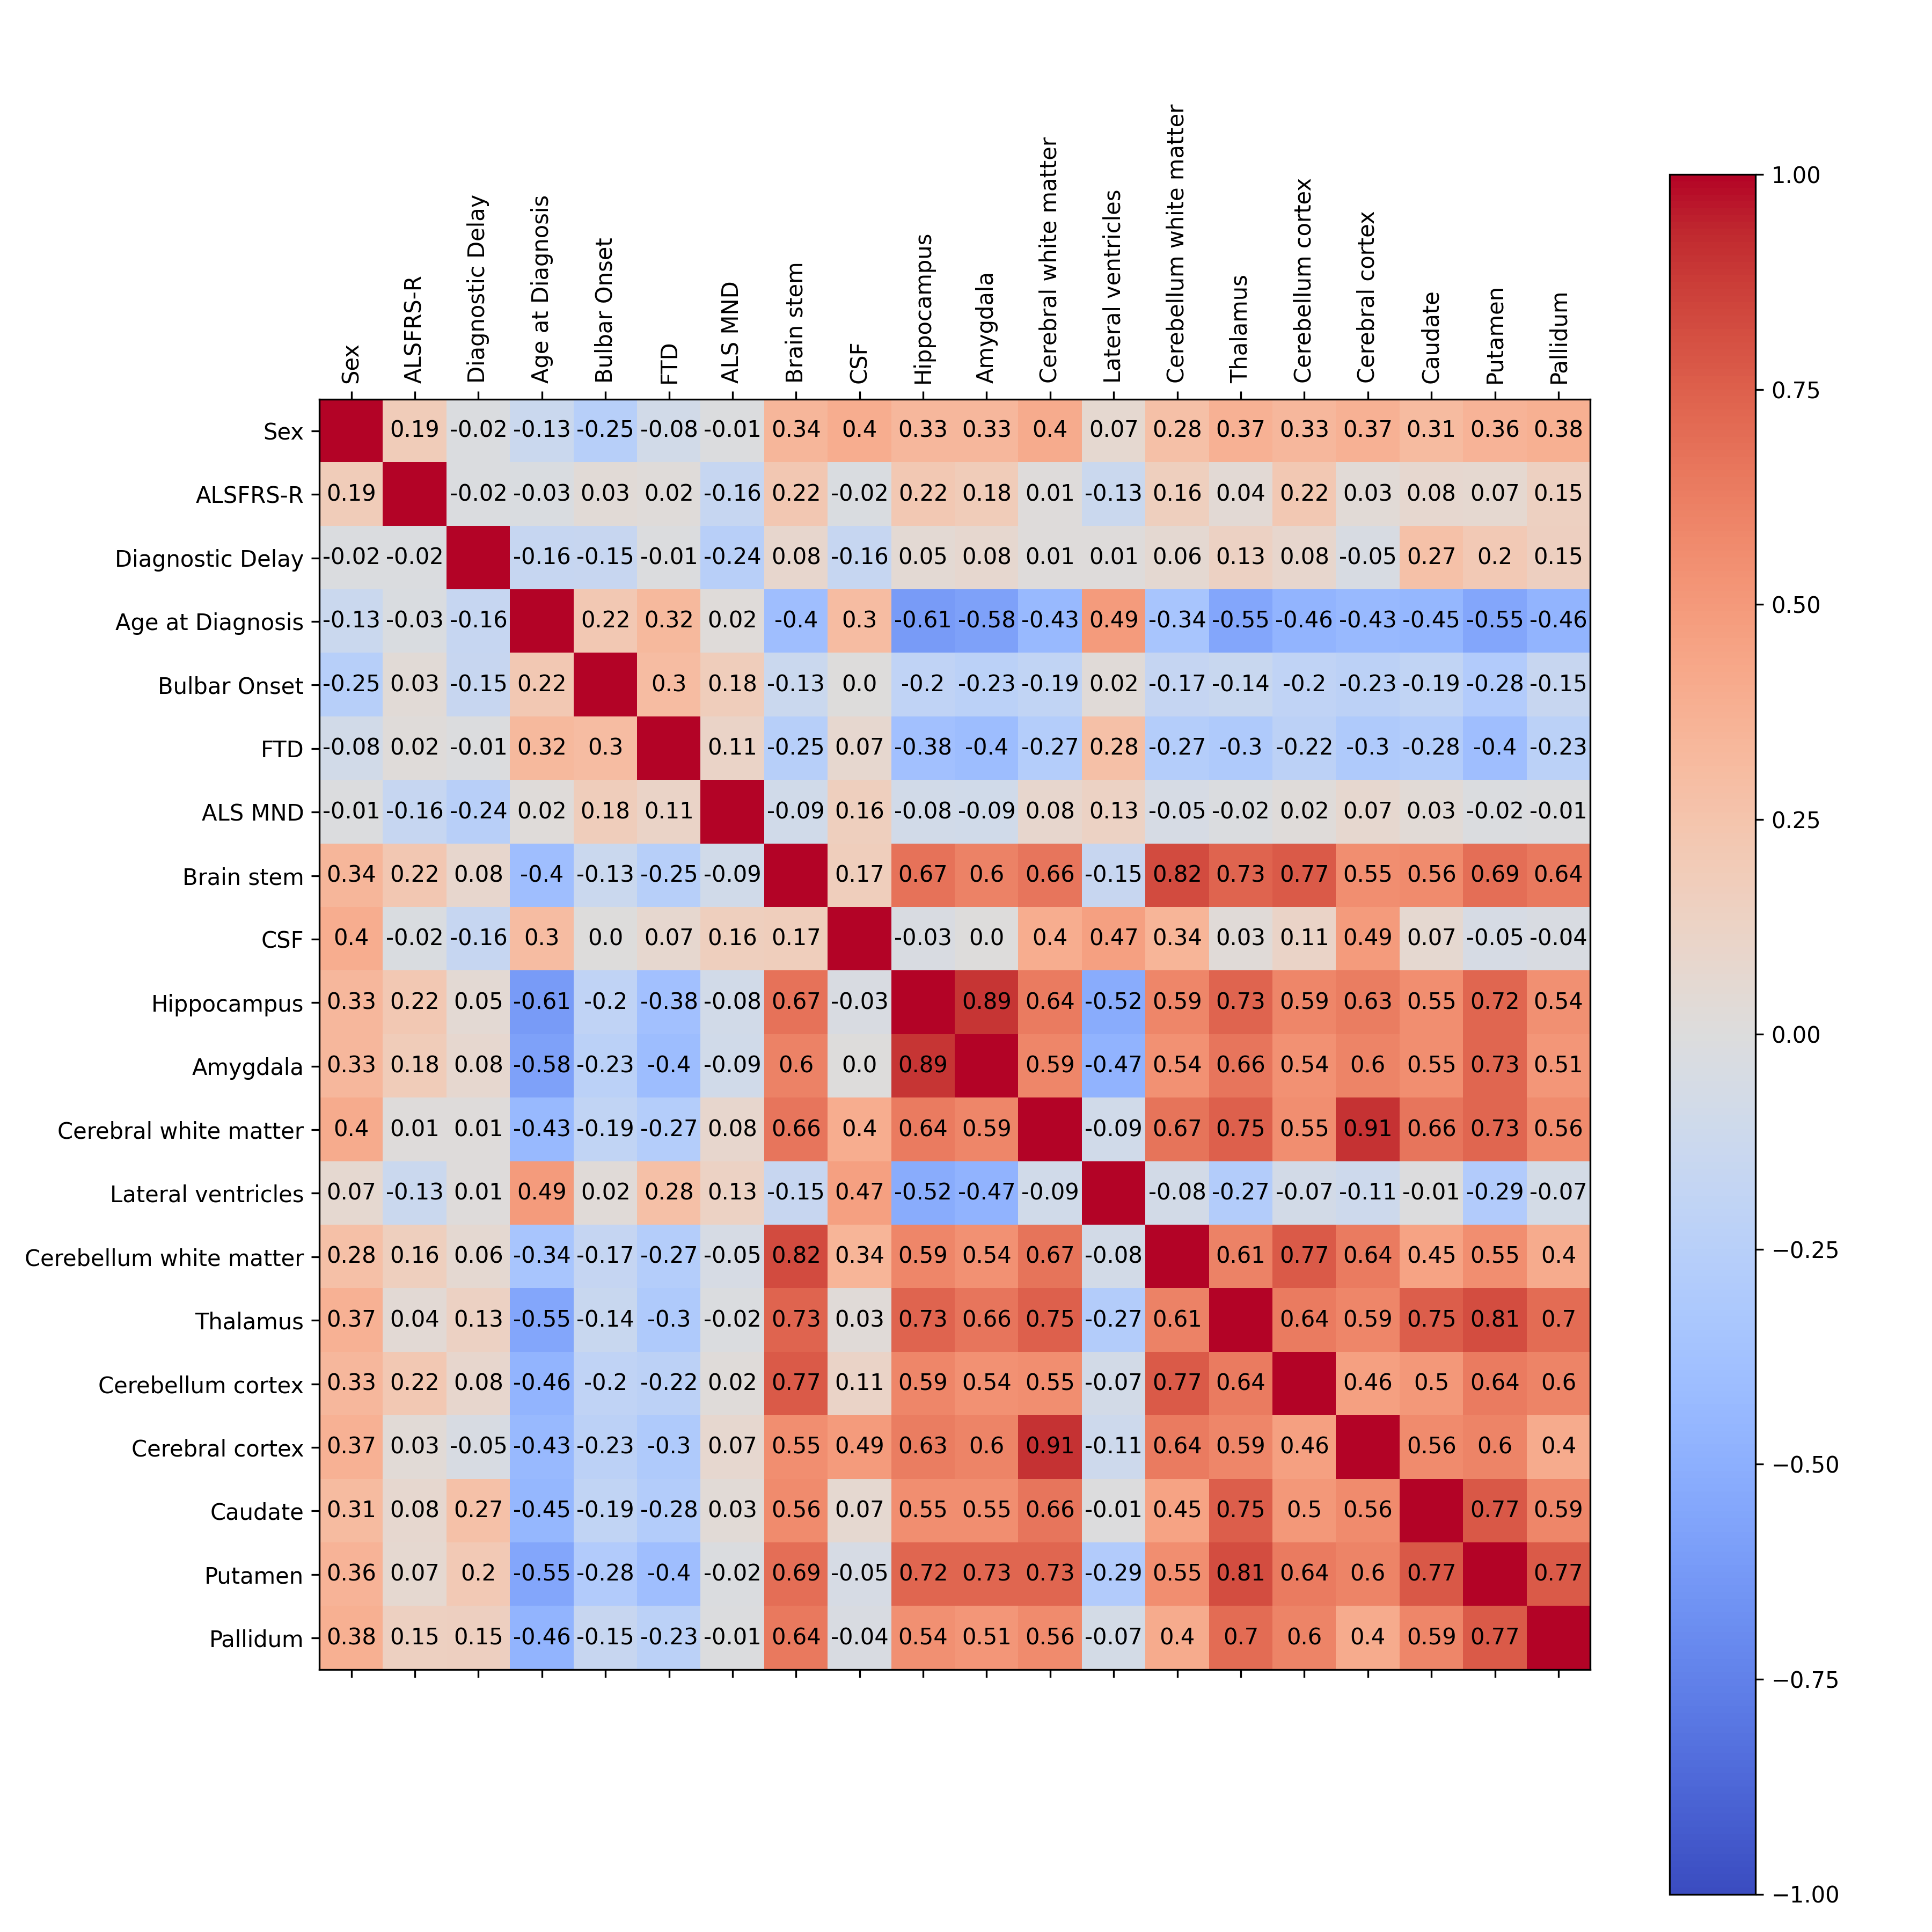
\includegraphics[width=\textwidth]{figures/multimodal_correlation}
    \caption{Correlations of all of the features included in the multimodal multivariable Cox proportional hazards model in Chapter~\ref{cox_proportional_hazards_model}, calculated with Pearson's correlation coefficient.}
    \label{fig:multimodalcorrelations}
\end{figure}

\chapter{Fusion Model Architectures}
\label{appendix:fusion_model_architectures}

\begin{figure}[h]
    \centering
    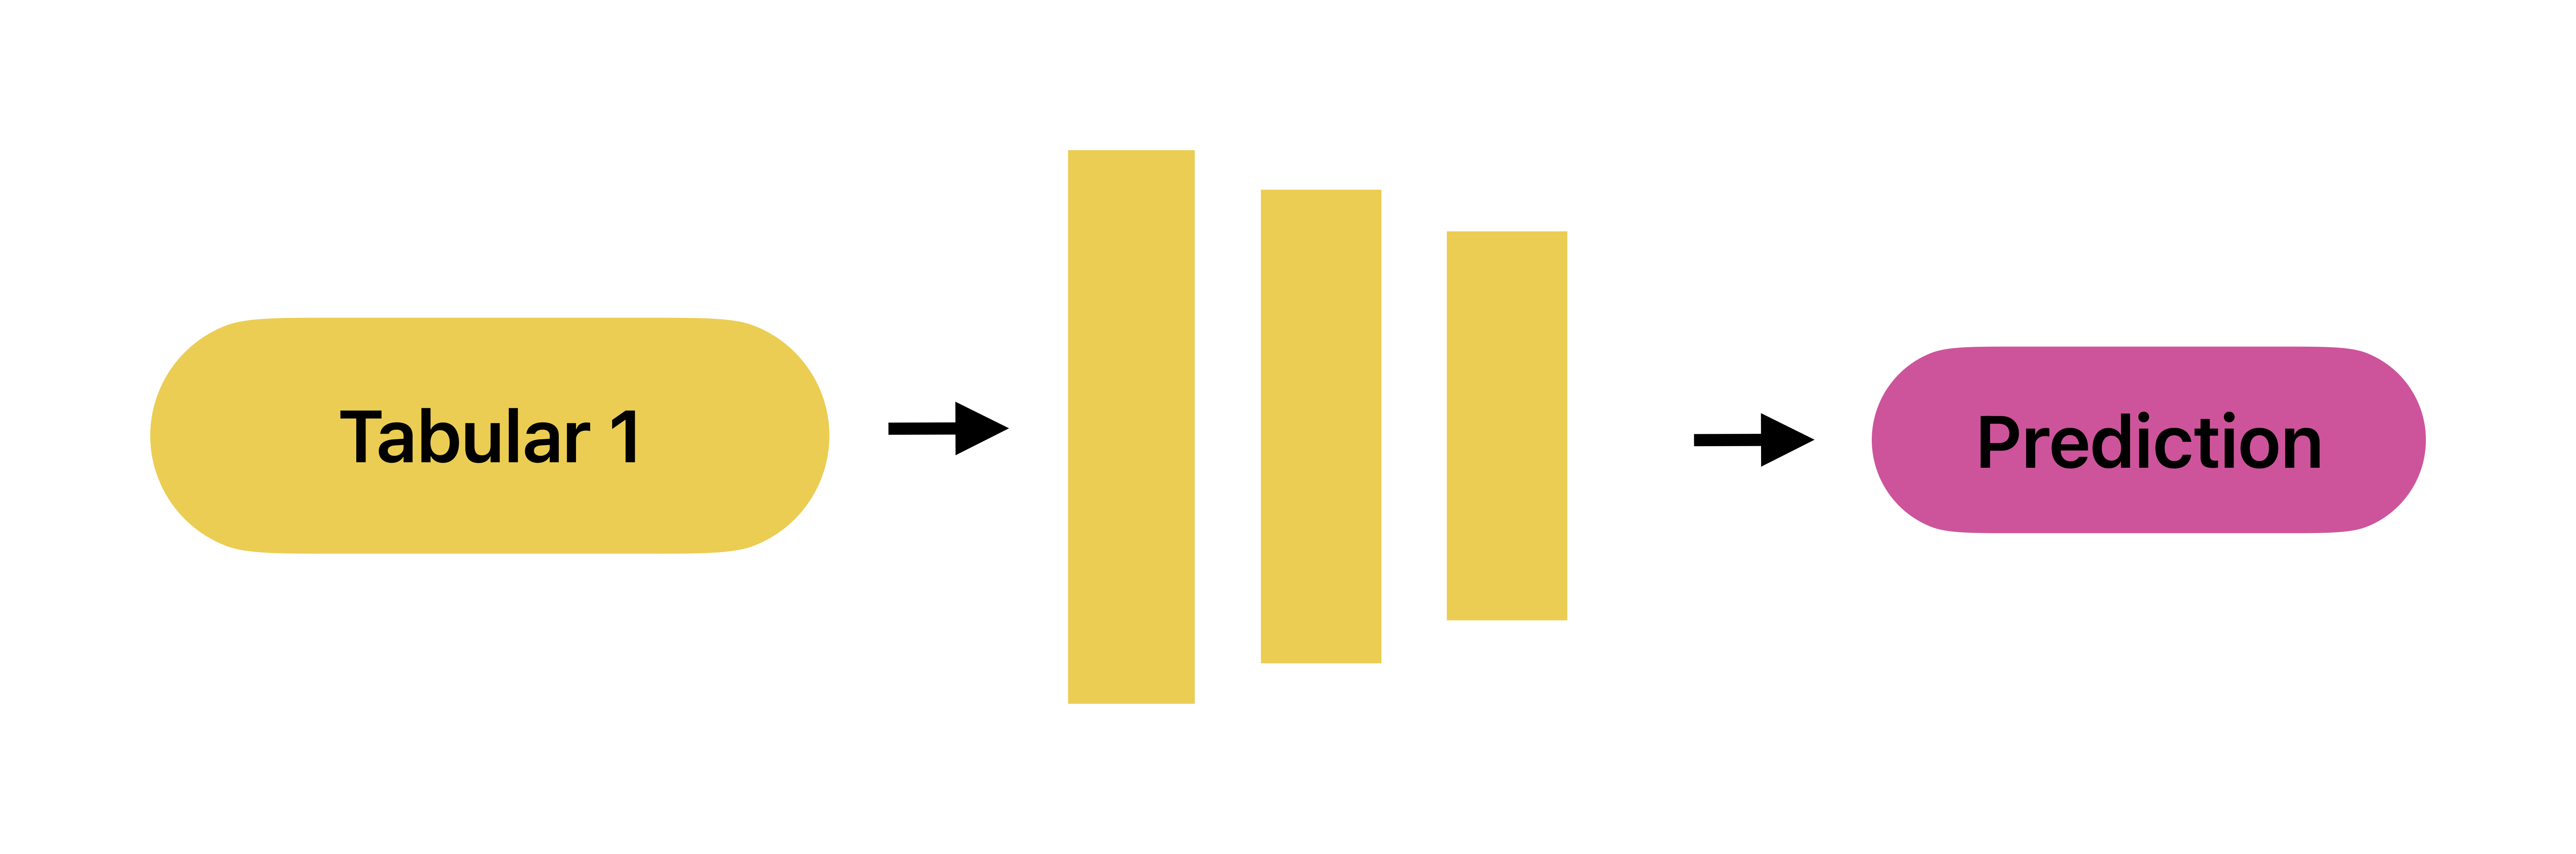
\includegraphics[width=0.8\linewidth]{figures//diagrams/Tabular1Unimodal}
    \caption[Clinical-only model architecture diagram.]{Clinical-only model architecture diagram from the Fusilli documentation~\cite{townendFlorencejtFusilliFusilli2024}.}
    \label{fig:tabular1}
\end{figure}

\begin{figure}[h]
    \centering
    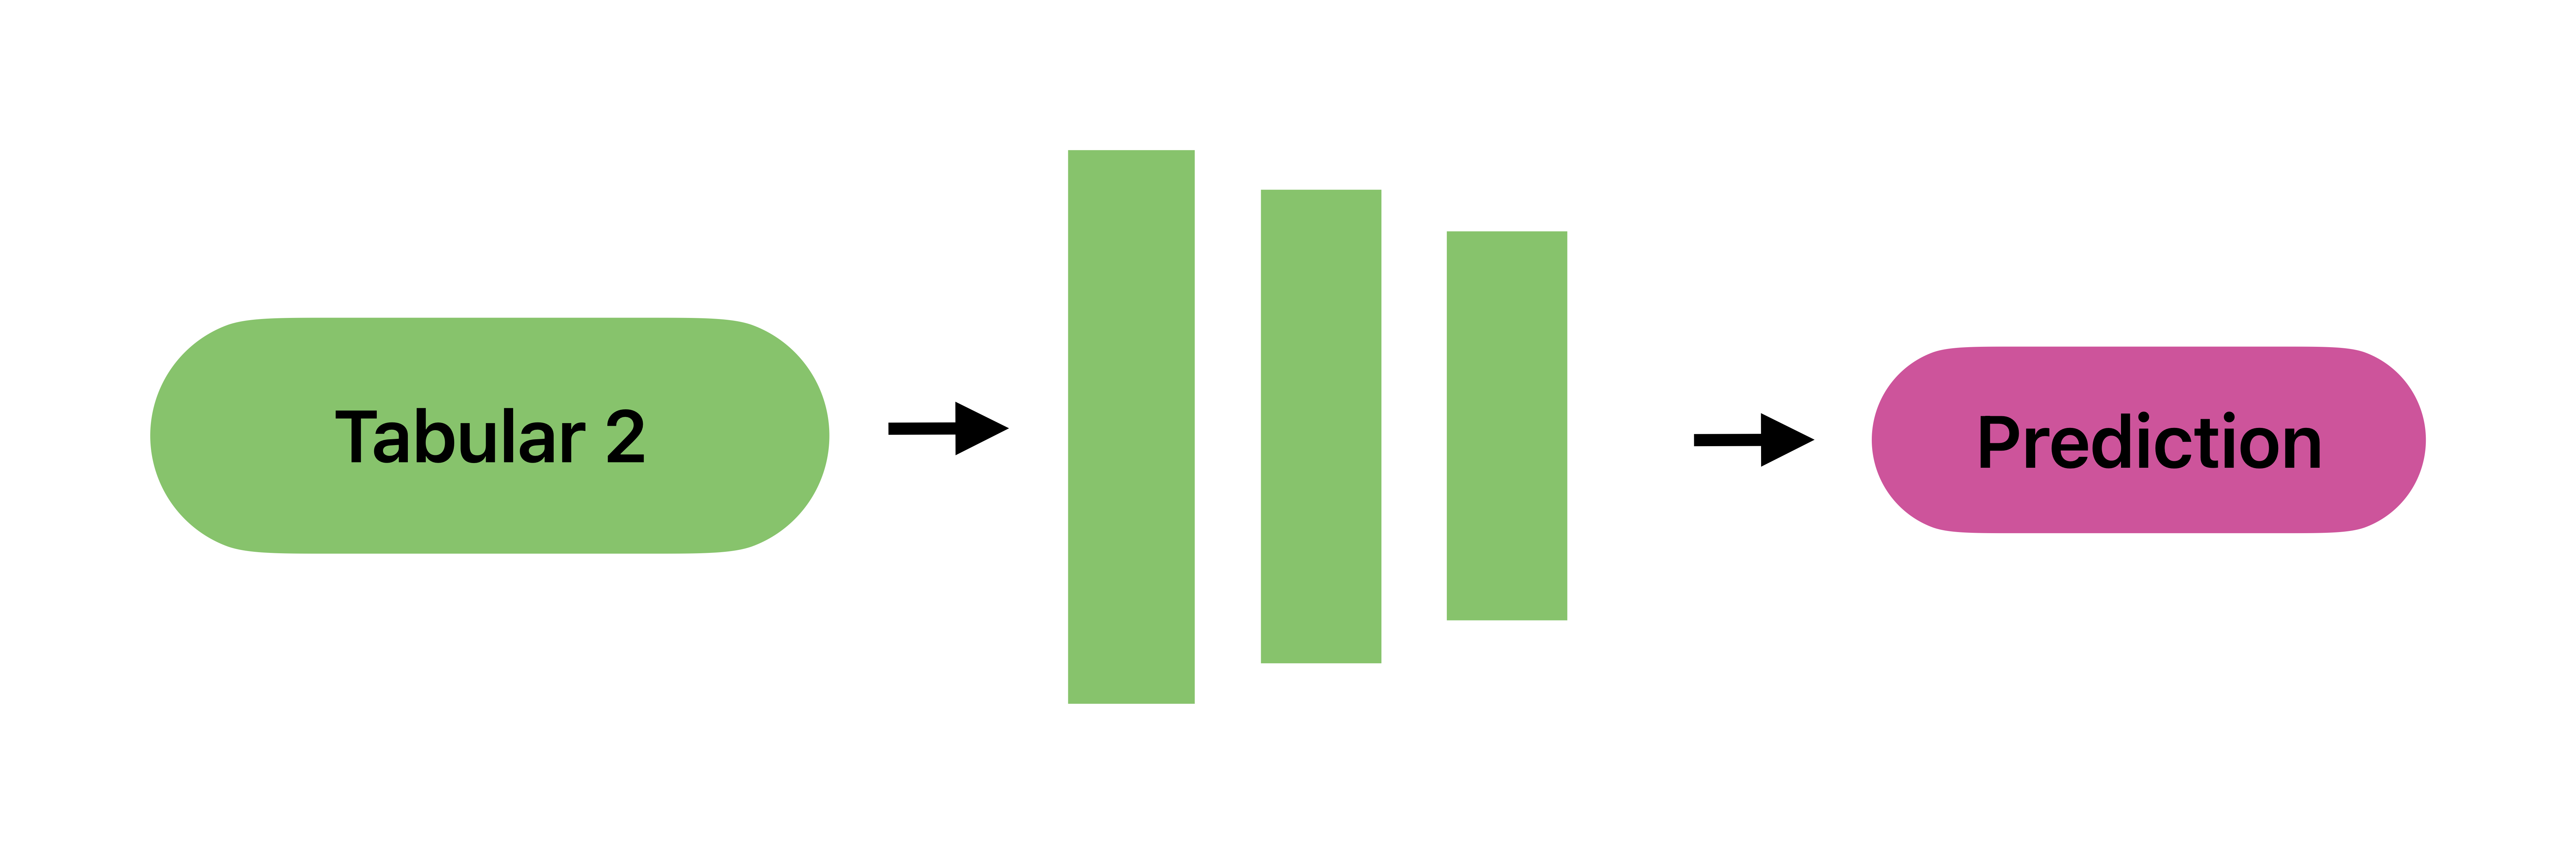
\includegraphics[width=0.8\linewidth]{figures//diagrams/Tabular2Unimodal}
    \caption[Imaging-only model architecture diagram.]{Imaging-only model architecture diagram from the Fusilli documentation~\cite{townendFlorencejtFusilliFusilli2024}.}
    \label{fig:tabular2}
\end{figure}

\begin{figure}[h]
    \centering
    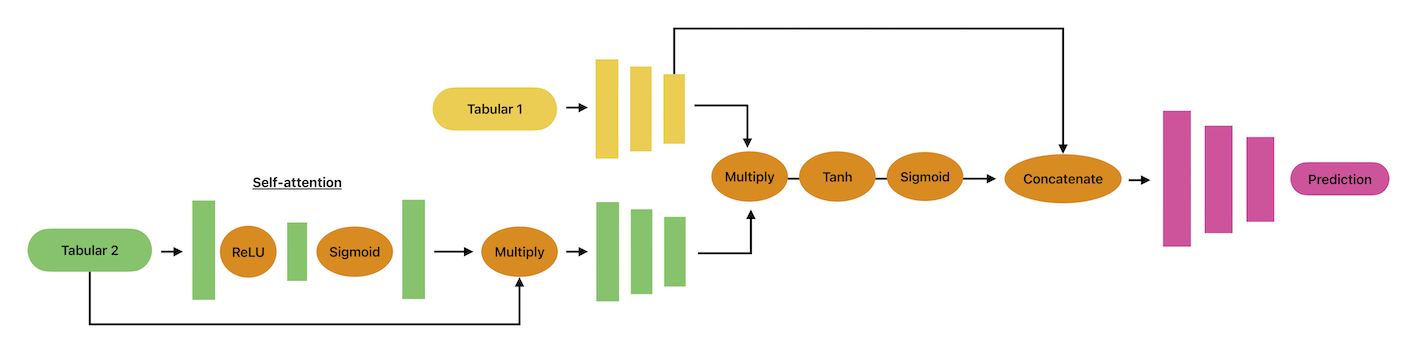
\includegraphics[width=1\linewidth]{figures//diagrams/ActivationandSelfAttention}
    \caption[Activation and Self-Attention model architecture diagram.]{Activation and Self-Attention model architecture diagram from the Fusilli documentation~\cite{townendFlorencejtFusilliFusilli2024}.}
    \label{fig:activationandselfattention}
\end{figure}


\begin{figure}[h]
    \centering
    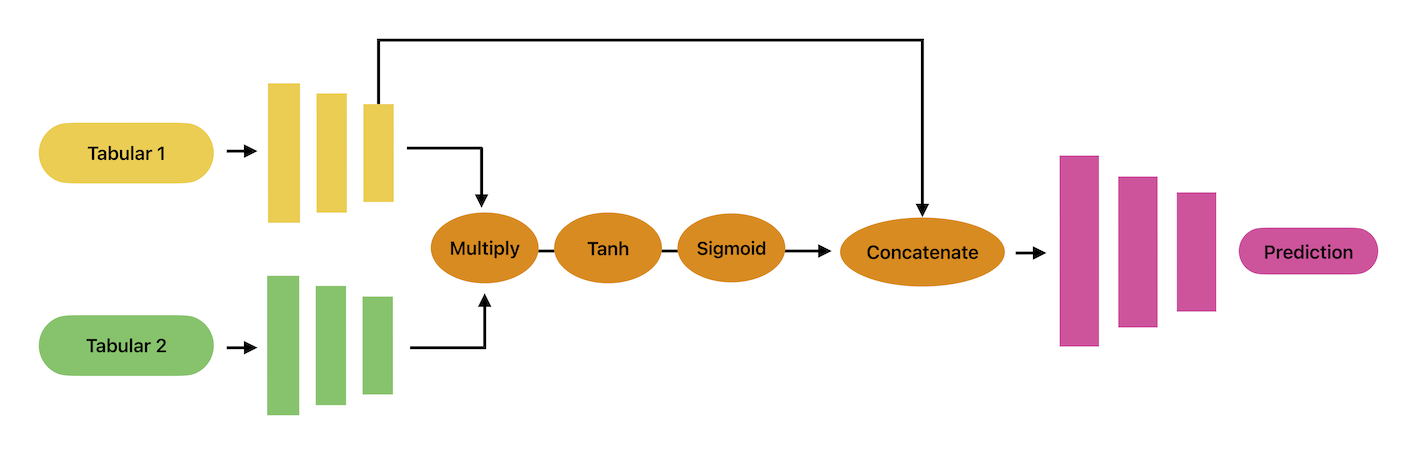
\includegraphics[width=1\linewidth]{figures//diagrams/ActivationFusion}
    \caption[Activation fusion model architecture diagram.]{Activation fusion model architecture diagram from the Fusilli documentation~\cite{townendFlorencejtFusilliFusilli2024}.}
    \label{fig:ActivationFusion}
\end{figure}

\begin{figure}[h]
    \centering
    
\includegraphics[width=1\linewidth]{figures//diagrams/ConcatTabularData}
    \caption[Concatenating tabular data model architecture diagram.]{Concatenating tabular data model architecture diagram from the Fusilli documentation~\cite{townendFlorencejtFusilliFusilli2024}.}
    \label{fig:ConcatTabularData}
\end{figure}

\begin{figure}[h]
    \centering
    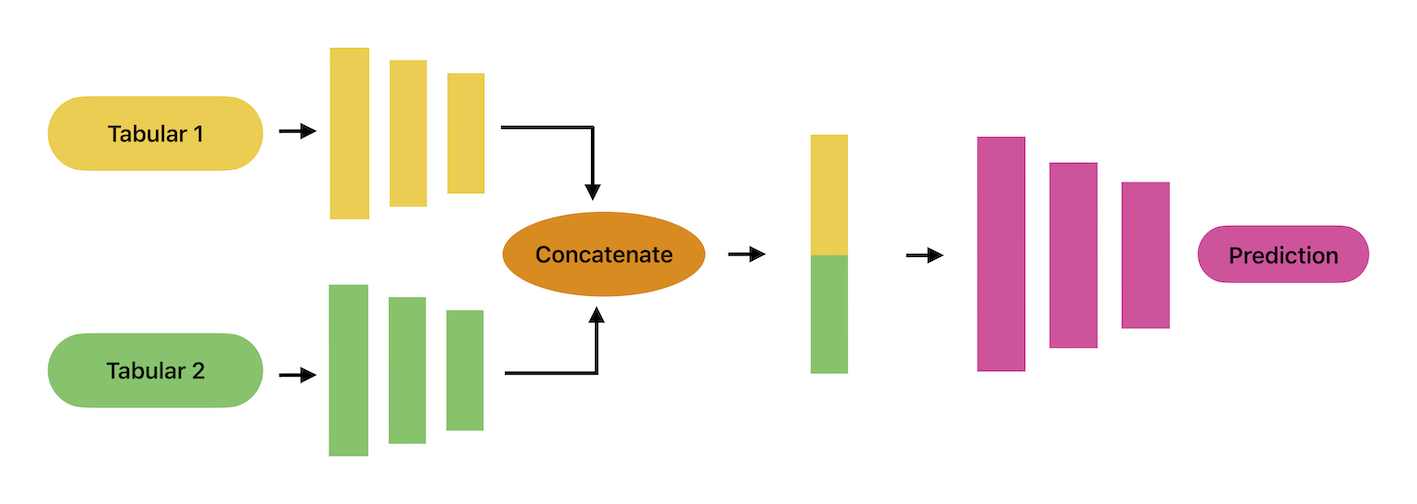
\includegraphics[width=1\linewidth]{figures//diagrams/ConcatTabularFeatureMaps}
    \caption[Concatenating tabular feature maps model architecture diagram.]{Concatenating tabular feature maps model architecture diagram from the Fusilli documentation~\cite{townendFlorencejtFusilliFusilli2024}.}
    \label{fig:ConcatTabularFeatureMaps}
\end{figure}

\begin{figure}[h]
    \centering
    \includegraphics[width=1\linewidth]{figures//diagrams/MCVAE}
    \caption[Multi-channel variational autoencoder model architecture diagram.]{Multi-channel variational autoencoder model architecture diagram from the Fusilli documentation~\cite{townendFlorencejtFusilliFusilli2024}.}
    \label{fig:MCVAE}
\end{figure}

\begin{figure}[h]
    \centering
    \includegraphics[width=1\linewidth]{figures//diagrams/TabularChannelwiseAttention}
    \caption[Channel-wise attention model architecture diagram.]{Channel-wise attention model architecture diagram from the Fusilli documentation~\cite{townendFlorencejtFusilliFusilli2024}.}
    \label{fig:TabularChannelwiseAttention}
\end{figure}

\begin{figure}[h]
    \centering
    \includegraphics[width=0.8\linewidth]{figures//diagrams/TabularCrossmodalAttention}
    \caption[Crossmodal attention model architecture diagram.]{Crossmodal attention model architecture diagram from the Fusilli documentation~\cite{townendFlorencejtFusilliFusilli2024}.}
    \label{fig:TabularCrossmodalAttention}
\end{figure}

\begin{figure}[h]
    \centering
    
\includegraphics[width=1\linewidth]{figures//diagrams/TabularDecision}
    \caption[Decision fusion model architecture diagram.]{Decision fusion model architecture diagram from the Fusilli documentation~\cite{townendFlorencejtFusilliFusilli2024}.}
    \label{fig:TabularDecision}
\end{figure}

%(stuff)
%
%\chapter{Another Appendix About Things}
%\label{appendixlabel2}
%(things)
%
%\chapter{Colophon}
%\label{appendixlabel3}
%\textit{This is a description of the tools you used to make your thesis. It helps people make future documents, reminds you, and looks good.}
%
%\textit{(example)} This document was set in the Times Roman typeface using \LaTeX\ and Bib\TeX , composed with a text editor.
 % description of document, e.g. type faces, TeX used, TeXmaker, packages and things used for figures. Like a computational details section.
% e.g. http://tex.stackexchange.com/questions/63468/what-is-best-way-to-mention-that-a-document-has-been-typeset-with-tex#63503

% Side note:
%http://tex.stackexchange.com/questions/1319/showcase-of-beautiful-typography-done-in-tex-friends

% You could separate these out into different files if you have
%  particularly large appendices.

% Actually generates your bibliography. The fact that \include is 
% the last thing before this ensures that it is on a clear page.
\bibliography{example}

% All done. \o/
\end{document}
